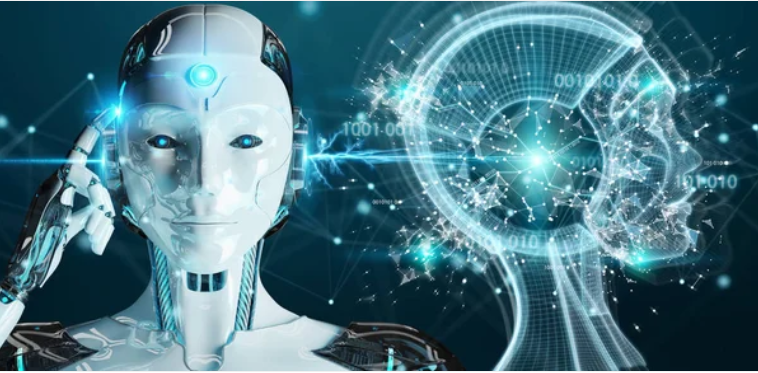
\includegraphics[width=8.49444in,height=4.14861in]{14-Logique/Cours/pandoc/media/image1.png}

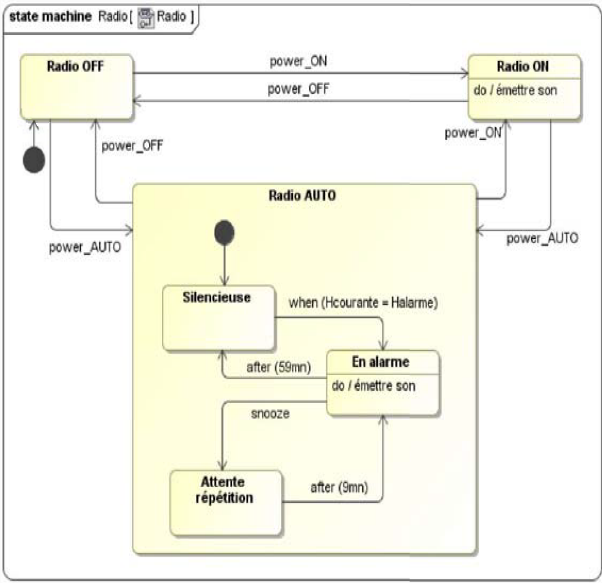
\includegraphics[width=2.73333in,height=2.65in]{14-Logique/Cours/pandoc/media/image3.png}

Cycle 8 : Analyser, Modéliser, Expérimenter et Résoudre les systèmes à évènements discrets

\textbf{Logique combinatoire, logique séquentielle, graphes d'états, communication réseau}

Thomas Lusseau

Lycée Robert Doisneau - ATS

\hypertarget{table-des-matiuxe8res}{%
\section*{\texorpdfstring{\textbf{Table des matières}}{Table des matières}}\label{table-des-matiuxe8res}}
\addcontentsline{toc}{section}{\textbf{Table des matières}}

\protect\hyperlink{guxe9nuxe9ralituxe9s-sur-les-systuxe8mes-logiques-combinatoires}{1. Généralités sur les systèmes logiques combinatoires {[}4{]}(\#généralités-sur-les-systèmes-logiques-combinatoires)}

\protect\hyperlink{symboles-et-notations}{1.1. Symboles et notations {[}4{]}(\#symboles-et-notations)}

\protect\hyperlink{duxe9marche-de-synthuxe8se-dun-systuxe8me-combinatoire}{1.2. Démarche de synthèse d'un système combinatoire {[}4{]}(\#démarche-de-synthèse-dun-système-combinatoire)}

\protect\hyperlink{table-de-vuxe9rituxe9}{1.3. Table de vérité {[}5{]}(\#table-de-vérité)}

\protect\hyperlink{equation-logique-uxe0-partir-de-la-table-de-vuxe9rituxe9}{1.4. Equation logique à partir de la table de vérité {[}8{]}(\#equation-logique-à-partir-de-la-table-de-vérité)}

\protect\hyperlink{ruxe8gles-de-lalguxe8bre-de-boole}{1.5. Règles de l'algèbre de Boole {[}8{]}(\#règles-de-lalgèbre-de-boole)}

\protect\hyperlink{moduxe9lisation-et-repruxe9sentation-des-opuxe9rateurs-logiques}{1.6. Modélisation et représentation des opérateurs logiques {[}9{]}(\#modélisation-et-représentation-des-opérateurs-logiques)}

\protect\hyperlink{optimisation-de-luxe9quation-logique}{1.7. Optimisation de l'équation logique {[}10{]}(\#optimisation-de-léquation-logique)}

\protect\hyperlink{synthuxe8se-de-luxe9quation-logique}{1.8. Synthèse de l'équation logique {[}10{]}(\#synthèse-de-léquation-logique)}

\protect\hyperlink{fonctions-combinatoires-particuliuxe8res}{1.9. Fonctions combinatoires particulières {[}12{]}(\#fonctions-combinatoires-particulières)}

\protect\hyperlink{technologie-des-circuits-intuxe9gruxe9s}{1.10. Technologie des circuits intégrés {[}18{]}(\#technologie-des-circuits-intégrés)}

\protect\hyperlink{systuxe8mes-uxe0-uxe9vuxe8nements-discrets-sed}{2. Systèmes à évènements Discrets (SED) {[}22{]}(\#systèmes-à-évènements-discrets-sed)}

\protect\hyperlink{exemple-introductif}{2.1. Exemple introductif {[}22{]}(\#exemple-introductif)}

\protect\hyperlink{systuxe8mes-suxe9quentiels}{2.2. Systèmes séquentiels {[}23{]}(\#systèmes-séquentiels)}

\protect\hyperlink{diagramme-duxe9tat-stm}{2.3. Diagramme d'état~(stm) {[}24{]}(\#diagramme-détat-stm)}

\protect\hyperlink{duxe9marche-de-moduxe9lisation-du-comportement-suxe9quentiel-dun-systuxe8me-par-un-graphe-duxe9tats}{2.4. Démarche de modélisation du comportement séquentiel d'un système par un graphe d'états {[}25{]}(\#démarche-de-modélisation-du-comportement-séquentiel-dun-système-par-un-graphe-détats)}

\protect\hyperlink{uxe9tat-et-ses-activituxe9s-associuxe9es}{2.5. État et ses activités associées {[}25{]}(\#état-et-ses-activités-associées)}

\protect\hyperlink{franchissement-des-transitions}{2.6. Franchissement des transitions {[}27{]}(\#franchissement-des-transitions)}

\protect\hyperlink{evuxe8nement}{2.7. Evènement {[}28{]}(\#evènement)}

\protect\hyperlink{garde}{2.8. Garde {[}28{]}(\#garde)}

\protect\hyperlink{equation-logique}{2.9. Equation logique {[}29{]}(\#equation-logique)}

\protect\hyperlink{effet}{2.10. Effet {[}29{]}(\#effet)}

\protect\hyperlink{pseudos-uxe9tats}{2.11. Pseudos-états {[}30{]}(\#pseudos-états)}

\protect\hyperlink{uxe9tat-composite}{2.12. État composite {[}33{]}(\#état-composite)}

\protect\hyperlink{historique-dun-uxe9tat-composite}{2.13. Historique d'un état composite {[}34{]}(\#historique-dun-état-composite)}

\protect\hyperlink{uxe9tat-composite-orthogonal}{2.14. État composite orthogonal {[}34{]}(\#état-composite-orthogonal)}

\protect\hyperlink{diagramme-de-suxe9quence-sd}{3. Diagramme de séquence~(sd) {[}38{]}(\#diagramme-de-séquence-sd)}

\protect\hyperlink{diagramme-de-suxe9quence}{3.1. Diagramme de séquence {[}38{]}(\#diagramme-de-séquence)}

\protect\hyperlink{codeur-incremental-et-absolu}{4. CODEUR INCREMENTAL ET ABSOLU {[}39{]}(\#codeur-incremental-et-absolu)}

\protect\hyperlink{familles-de-capteurs}{4.1. Familles de capteurs {[}39{]}(\#familles-de-capteurs)}

\protect\hyperlink{vocabulaire-de-muxe9trologie}{4.2. Vocabulaire de métrologie {[}40{]}(\#vocabulaire-de-métrologie)}

\protect\hyperlink{les-codeurs}{4.3. Les codeurs {[}40{]}(\#les-codeurs)}

\protect\hyperlink{reseaux-et-bus-de-terrain}{5. RESEAUX ET BUS DE TERRAIN {[}45{]}(\#reseaux-et-bus-de-terrain)}

\protect\hyperlink{introduction-sur-les-donnuxe9es}{5.1. Introduction sur les données {[}45{]}(\#introduction-sur-les-données)}

\protect\hyperlink{qualituxe9-de-service-qos}{5.2. Qualité de service~: QoS {[}45{]}(\#qualité-de-service-qos)}

\protect\hyperlink{architecture-des-ruxe9seaux-de-communication}{5.3. Architecture des réseaux de communication {[}45{]}(\#architecture-des-réseaux-de-communication)}

\protect\hyperlink{couches-du-moduxe8le-osi}{5.4. Couches du modèle OSI {[}46{]}(\#couches-du-modèle-osi)}

\protect\hyperlink{les-supports-de-transmission}{5.5. Les supports de transmission {[}47{]}(\#les-supports-de-transmission)}

\protect\hyperlink{principemultiplexagemultiplexage}{5.6. Multiplexage {[}50{]}(\#principemultiplexagemultiplexage)}

\protect\hyperlink{les-erreurs-de-transmission}{5.7. Les erreurs de transmission {[}51{]}(\#les-erreurs-de-transmission)}

\protect\hyperlink{topologie-des-ruxe9seaux}{5.8. Topologie des réseaux {[}54{]}(\#topologie-des-réseaux)}

\protect\hyperlink{types-de-liaisons-des-ruxe9seaux-de-communication}{5.9. Types de liaisons des réseaux de communication {[}55{]}(\#types-de-liaisons-des-réseaux-de-communication)}

\protect\hyperlink{architecture-de-la-chauxeene-de-transmission}{5.10. Architecture de la chaîne de transmission {[}56{]}(\#architecture-de-la-chaîne-de-transmission)}

\protect\hyperlink{caractuxe9ristiques-de-la-transmission}{5.11. Caractéristiques de la transmission {[}57{]}(\#caractéristiques-de-la-transmission)}

\protect\hyperlink{protocoles-des-ruxe9seaux-de-communication}{5.1. Protocoles des réseaux de communication {[}58{]}(\#protocoles-des-réseaux-de-communication)}

\protect\hyperlink{sources}{6. Sources {[}71{]}(\#sources)}

\protect\hyperlink{_Toc130196631}{7. Exercices du chapitre {[}72{]}(\#\_Toc130196631)}

\hypertarget{guxe9nuxe9ralituxe9s-sur-les-systuxe8mes-logiques-combinatoires}{%
\subsection{Généralités sur les systèmes logiques combinatoires}\label{guxe9nuxe9ralituxe9s-sur-les-systuxe8mes-logiques-combinatoires}}

\hypertarget{symboles-et-notations}{%
\subsubsection{Symboles et notations}\label{symboles-et-notations}}

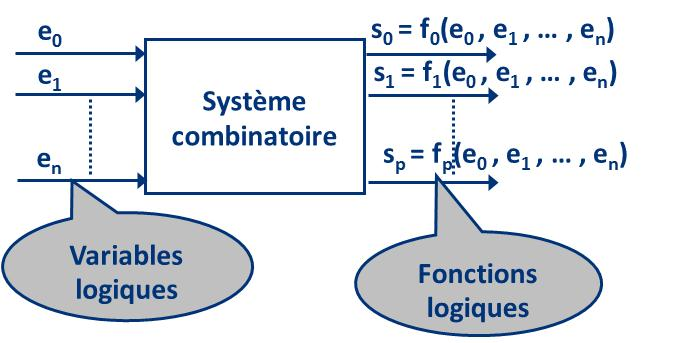
\includegraphics[width=3.10694in,height=1.57222in]{14-Logique/Cours/pandoc/media/image5.jpeg}Un \textbf{système combinatoire} est un système \textbf{logique} (ou booléen) traitant des informations sous \textbf{forme logique (ou booléenne)} et dont les \textbf{états des sorties sont \ul{exclusivement} définis à partir des entrées}.

On peut alors représenter un système combinatoire par un bloc entre les variables d'entrées et de sortie. Les sorties sont reliées aux entrées par une \textbf{fonction logique ne dépendant que des entrées.}

Les entrées et sorties d'un tel système sont des \textbf{variables logiques (ou binaires, ou booléennes)} qui ne peuvent prendre que \textbf{deux valeurs 0 ou 1} permettant de représenter l'état d'un objet :

\begin{itemize}
\item
  ouvert ou fermé;
\item
  vrai ou faux;
\item
  tension de 5V ou de 0V;
\item
  tout ou rien;
\item
  présent ou absent, \ldots{}
\end{itemize}

\textbf{L'état logique « 1 »} informe que l'entrée a été actionnée. \textbf{L'état logique « 0 »} informe que l'entrée n'a pas été actionnée.

\hypertarget{duxe9marche-de-synthuxe8se-dun-systuxe8me-combinatoire}{%
\subsubsection{Démarche de synthèse d'un système combinatoire}\label{duxe9marche-de-synthuxe8se-dun-systuxe8me-combinatoire}}

A partir du cahier des charges d'un système qui nous incite à mettre en œuvre un \textbf{système combinatoire}, on obtient un chronogramme, une \textbf{table de vérité} ou une \textbf{équation logique} décrivant le fonctionnement des sorties en fonction des entrées.

Pour arriver jusqu'à la \textbf{synthèse} (solution câblée -ou programmée -), on doit passer par différentes opérations~:

\begin{itemize}
\item
  La \textbf{table de vérité} ou \textbf{l'équation logique}~: elle traduit le \textgreater{} cahier des charges.
\item
  L\textbf{'optimisation}~: elle a pour but de réduire les \textbf{opérateurs \textgreater{} logiques} pour réaliser l'équation logique.
\item
  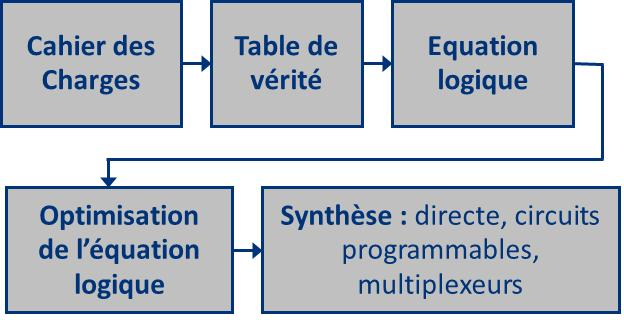
\includegraphics{14-Logique/Cours/pandoc/media/image6.jpeg}\{width=``2.1055555555555556in'' \textgreater{} height=``1.0798611111111112in''\} La \textbf{synthèse}~: c'est la \textgreater{} réalisation matérielle du circuit réalisant le système \textgreater{} combinatoire.
\end{itemize}

On peut alors représenter les différentes phases de la synthèse d'une fonction logique combinatoire par le schéma suivant~:

\begin{longtable}[]{@{}
  >{\raggedright\arraybackslash}p{(\columnwidth - 0\tabcolsep) * \real{1.0000}}@{}}
\toprule\noalign{}
\begin{minipage}[b]{\linewidth}\raggedright
\textbf{Table de vérité en code binaire :}


\includegraphics[width=2.37809in,height=3.40698in]{14 -Logique/Cours/pandoc/media/image7.jpeg}
\end{minipage} \\
\midrule\noalign{}
\endhead
\bottomrule\noalign{}
\endlastfoot
 \\
\end{longtable}

\hypertarget{table-de-vuxe9rituxe9}{%
\subsubsection{Table de vérité}\label{table-de-vuxe9rituxe9}}

Le fonctionnement d'un système combinatoire est décrit par une \textbf{table de vérité}. Elle permet de faire \textbf{correspondre l'état des sorties en fonction de l'état des entrées} et cela pour \textbf{toutes les combinaisons possibles des entrées}.

Pour un système combinatoire de \textbf{n entrées} il y aura \textbf{2\textsuperscript{n} combinaisons (ou cas)} possibles (3 entrées 8 combinaisons, 4 entrées 16 combinaisons, \ldots).

\textbf{L'équation logique de la sortie} peut alors être déterminée en recherchant toutes les \textbf{combinaisons d'entrées pour lesquelles la sortie vaut 1.}

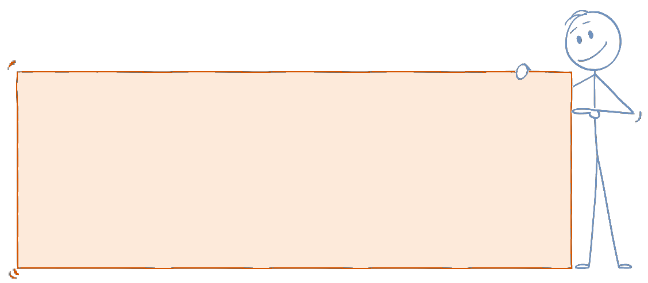
\includegraphics[width=3.71875in,height=1.51667in]{14-Logique/Cours/pandoc/media/image8.png}

\begin{longtable}[]{@{}
  >{\raggedright\arraybackslash}p{(\columnwidth - 2\tabcolsep) * \real{0.1250}}
  >{\raggedright\arraybackslash}p{(\columnwidth - 2\tabcolsep) * \real{0.8611}}@{}}
\toprule\noalign{}
\begin{minipage}[b]{\linewidth}\raggedright
\begin{quote}
{[}{]} (14-Lo gique/ Cours/ pandoc /media /image 10.png )\{widt h=``0.6 262696 850393 701in''

height =``0.65 083333 333333 34in''\}
\end{quote}
\end{minipage} & \begin{minipage}[b]{\linewidth}\raggedright

\includegraphics[width=1.45903in,height=1.11389in]{14-Logique/Co urs/pandoc/media/image11.jpeg}\textbf{Store SOMFY}

L\textquotesingle entreprise SOMFY propose toute une gamme de matériels "grand public" dont le store SOMFY fait partie.

Ce store est composé de cinq éléments~:

\begin{itemize}
\item
  Un store qui protège l\textquotesingle utilisateur des rayons du soleil.
\item
  Un opérateur tubulaire capable d\textquotesingle enrouler ou de dérouler le store.
\item
  Un capteur de vent qui détecte la présence de vent.
\item
  Un capteur solaire qui détecte la présence de soleil.
\item
  Un automatisme vent / soleil qui permet à l\textquotesingle utilisateur de commander en mode manuel ou en mode automatique le store.
\end{itemize}

\begin{center}

\includegraphics[width=3.27361in,height=1.80556in]{14-Logique/Co urs/pandoc/media/image12.jpeg}

sdf
\end{center}

Par mesure de sécurité (pour l\textquotesingle utilisateur comme pour le store), \ul{l\textquotesingle action du vent est toujours prioritaire sur l\textquotesingle action du soleil} et ce, aussi bien en mode automatique qu\textquotesingle en mode manuel. Le diagramme sagittal ci-dessous, présente les différents constituants de ce système.

\ul{Cahier des charges~:}

Si le vent devient supérieur à un seuil préréglé, le module de commande monte le store et le laisse en position haute. Cette fonction est prioritaire sur toutes les autres pour des raisons de sécurité.

En l'absence de vent, l'utilisateur peut commander la montée ou la descente du store par des inverseurs. Cette fonction manuelle est prioritaire sur la fonction soleil qui, lorsque la luminosité devient supérieure au seuil préréglé, provoque la descente du store.

Le schéma structurel est donné ci-dessous.

\begin{center}

\includegraphics[width=5.62503in,height=4.41667in]{14-Logique/C ours/pandoc/media/image13.jpeg}

sdf
\end{center}

\textbf{En vous aidant du cahier des charges, et de la présentation du système, lister les entrées et sorties du système.}

\textbf{Etablir la table de vérité du système effectuant le traitement numérique des informations (fonction FP4).}

\textbf{Déterminer l'équation logique de la sortie CD.}\strut
\end{minipage} \\
\midrule\noalign{}
\endhead
\bottomrule\noalign{}
\endlastfoot
& \\
\end{longtable}

\textbf{Etat logique indifférent « X » :}

Pour \textbf{certaines combinaisons d'entrées}, il peut arriver qu'on ne puisse \textbf{pas déterminer l'état de la sortie logique car la combinaison des entrées ne peut pas se produire ou qu'elle ne nous intéresse pas.}

Dans ces cas-là, il existe un \textbf{état logique appelé indifférent, noté « X » ou « - » qui peut prendre les valeurs « 0 » ou « 1 ».}

\hypertarget{equation-logique-uxe0-partir-de-la-table-de-vuxe9rituxe9}{%
\subsubsection{Equation logique à partir de la table de vérité}\label{equation-logique-uxe0-partir-de-la-table-de-vuxe9rituxe9}}

\textbf{L'équation logique d'une sortie} peut se déduire à partir de la table de vérité traduisant le cahier des charges. Il suffit alors de lister les combinaisons des entrées (reliées par un ET logique) pour lesquelles la sortie est activée (« 1 » logique) et de les séparer par un OU logique.

Soit un système combinatoire à deux entrées (a et b) et une sortie (S). La sortie est activée si une action est faite sur b \ul{ET} pas sur a \ul{OU} si une action est faite sur a et sur b. Ceci se traduit par l'équation logique : \(S = b.\overline{a} + b.a\)

Pour réaliser la synthèse de cette équation logique, il faut définir deux \textbf{opérateurs logiques,} On les nomme \textbf{BOOLEEN}. A l'opérateur \textbf{ET} est associé l'opérateur mathématique «~\textbf{.}~». A l'opérateur \textbf{OU} est associé l'opérateur mathématique «\textbf{~+}~». \textbf{Et nous obtenons l'appellation «~ALGEBRE DE BOOLE~»}

\hypertarget{ruxe8gles-de-lalguxe8bre-de-boole}{%
\subsubsection{Règles de l'algèbre de Boole}\label{ruxe8gles-de-lalguxe8bre-de-boole}}

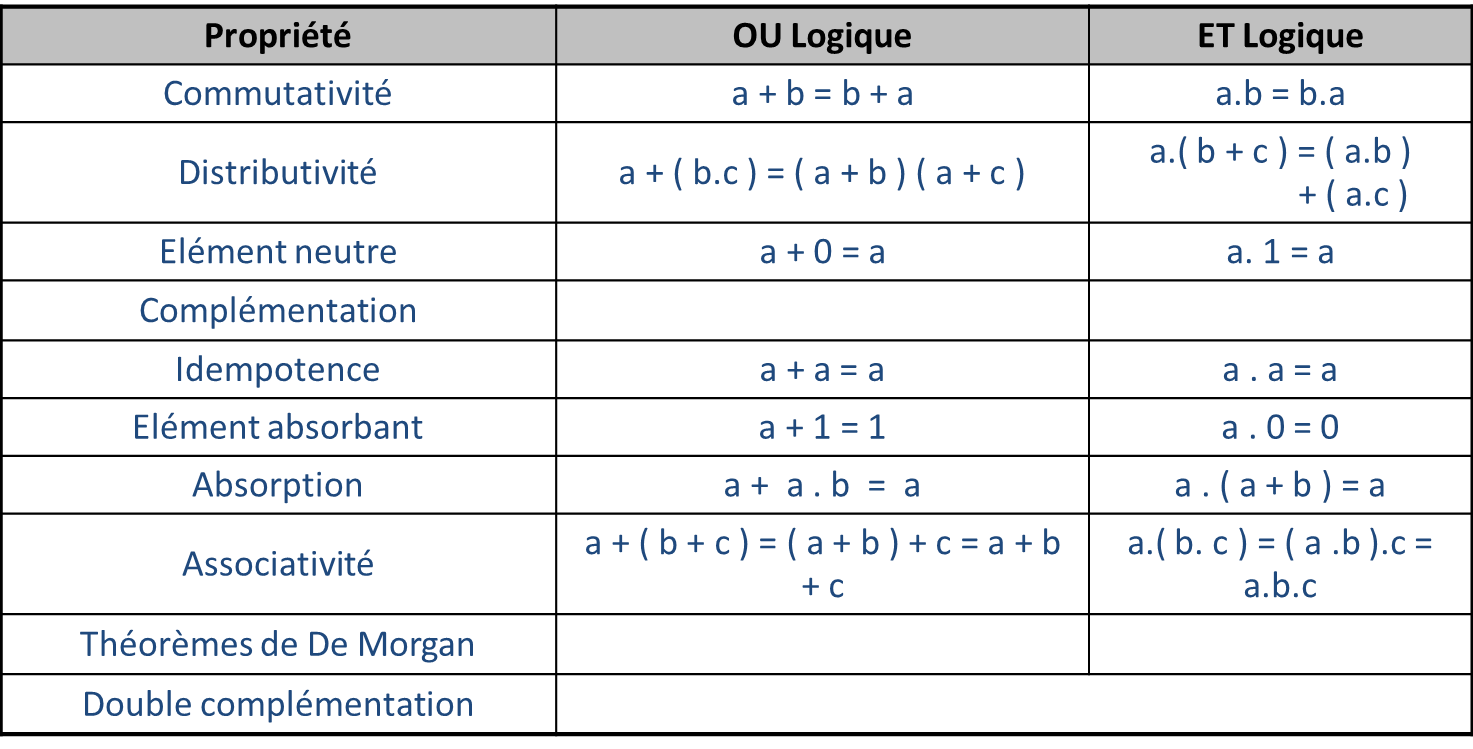
\includegraphics[width=6.26736in,height=3.09722in]{14-Logique/Cours/pandoc/media/image14.png}
\includegraphics[width=1.16458in,height=0.34722in]{14-Logique/Cours/pandoc/media/image15.wmf}
\includegraphics[width=0.82431in,height=0.38889in]{14-Logique/Cours/pandoc/media/image16.wmf}


\includegraphics{14-Logique/Cours/pandoc/media/image17.wmf}
\includegraphics[width=0.5in,height=0.22153in]{14-Logique/Cours/pandoc/media/image18.wmf}


\includegraphics{14-Logique/Cours/pandoc/media/image19.wmf}
\includegraphics[width=0.75556in,height=0.225in]{14-Logique/Cours/pandoc/media/image20.wmf}


\includegraphics[width=0.325in,height=0.24722in]{14-Logique/Cours/pandoc/media/image21.wmf}


\includegraphics[width=5.38125in,height=0.64931in]{14-Logique/Cours/pandoc/media/image22.jpeg}

\hypertarget{moduxe9lisation-et-repruxe9sentation-des-opuxe9rateurs-logiques}{%
\subsubsection{Modélisation et représentation des opérateurs logiques}\label{moduxe9lisation-et-repruxe9sentation-des-opuxe9rateurs-logiques}}

On utilise différentes représentations pour les opérateurs logiques~:

\begin{itemize}
\item
  \textbf{Les symboles (normes IEC --européenne -- et ANSI -- américaine --);}
\item
  Les \textbf{schémas logiques à contact} (équivalent électrique)
\item
  \textbf{L'équation logique} (ou booléenne);
\item
  La \textbf{table de vérité} (état des sorties en fonction des entrées);
\item
  Les \textbf{chronogrammes} (évolution de la variable logique dans le temps.
\end{itemize}

\begin{longtable}[]{@{}
  >{\raggedright\arraybackslash}p{(\columnwidth - 8\tabcolsep) * \real{0.2838}}
  >{\raggedright\arraybackslash}p{(\columnwidth - 8\tabcolsep) * \real{0.2027}}
  >{\raggedright\arraybackslash}p{(\columnwidth - 8\tabcolsep) * \real{0.2027}}
  >{\raggedright\arraybackslash}p{(\columnwidth - 8\tabcolsep) * \real{0.1216}}
  >{\raggedright\arraybackslash}p{(\columnwidth - 8\tabcolsep) * \real{0.1486}}@{}}
\toprule\noalign{}
\begin{minipage}[b]{\linewidth}\raggedright
\textbf{Schéma électrique}
\end{minipage} & \begin{minipage}[b]{\linewidth}\raggedright
\textbf{Symbole}
\end{minipage} & \begin{minipage}[b]{\linewidth}\raggedright
\textbf{Table de vérité}
\end{minipage} & \begin{minipage}[b]{\linewidth}\raggedright
\begin{itemize}
\tightlist
\item
  *Nom**
\end{itemize}
\end{minipage} & \begin{minipage}[b]{\linewidth}\raggedright
\textbf{Eq uation}
\end{minipage} \\
\midrule\noalign{}
\endhead
\bottomrule\noalign{}
\endlastfoot
\textbf{a L} & & \begin{minipage}[t]{\linewidth}\raggedright
\begin{longtable}[]{@{}
  >{\raggedright\arraybackslash}p{(\columnwidth - 2\tabcolsep) * \real{0.0694}}
  >{\raggedright\arraybackslash}p{(\columnwidth - 2\tabcolsep) * \real{0.0694}}@{}}
\toprule\noalign{}
\endhead
\bottomrule\noalign{}
\endlastfoot
a & L \\
0 & 1 \\
1 & 0 \\
\end{longtable}
\end{minipage} & \textbf{NON ( NOT)} & \textbf{L=a} \\
\textbf{a L} & & \begin{minipage}[t]{\linewidth}\raggedright
\begin{longtable}[]{@{}
  >{\raggedright\arraybackslash}p{(\columnwidth - 2\tabcolsep) * \real{0.0694}}
  >{\raggedright\arraybackslash}p{(\columnwidth - 2\tabcolsep) * \real{0.0694}}@{}}
\toprule\noalign{}
\endhead
\bottomrule\noalign{}
\endlastfoot
a & L \\
0 & 0 \\
1 & 1 \\
\end{longtable}
\end{minipage} & \textbf{OUI ( YES)} & \textbf{L=a} \\
\textbf{a b L} & & \begin{minipage}[t]{\linewidth}\raggedright
\begin{longtable}[]{@{}rl@{}}
\toprule\noalign{}
---- & --- --- \\
\midrule\noalign{}
\endhead
\bottomrule\noalign{}
\endlastfoot
**a & ** * \\
*b** & \textbf{L} \\
\end{longtable}

\textbf{0} \emph{ }0** \textbf{0}

\textbf{0} \emph{ }1** \textbf{0}

\textbf{1} \emph{ }0** \textbf{0}

\textbf{1} \emph{ }1** \textbf{1}

\begin{center}\rule{0.5\linewidth}{0.5pt}\end{center}

\begin{center}\rule{0.5\linewidth}{0.5pt}\end{center}
\end{minipage} & \textbf{ET ( AND)} & \begin{minipage}[t]{\linewidth}\raggedright
\begin{itemize}
\tightlist
\item
  *L=a.b**
\end{itemize}
\end{minipage} \\
\textbf{a L}

\textbf{b} & & \begin{minipage}[t]{\linewidth}\raggedright
\begin{longtable}[]{@{}rl@{}}
\toprule\noalign{}
---- & --- --- \\
\midrule\noalign{}
\endhead
\bottomrule\noalign{}
\endlastfoot
**a & ** * \\
*b** & \textbf{L} \\
\end{longtable}

\textbf{0} \emph{ }0** \textbf{1}

\textbf{0} \emph{ }1** \textbf{1}

\textbf{1} \emph{ }0** \textbf{1}

\textbf{1} \emph{ }1** \textbf{0}

\begin{center}\rule{0.5\linewidth}{0.5pt}\end{center}

\begin{center}\rule{0.5\linewidth}{0.5pt}\end{center}
\end{minipage} & \begin{minipage}[t]{\linewidth}\raggedright
\begin{itemize}
\tightlist
\item
  *NONET (N AND)**
\end{itemize}
\end{minipage} & \textbf{L =a .b=a+b} \\
\textbf{a L}

\textbf{b} & \includegraphics{14-Log ique/Cours/p andoc/media/ image23.wmf} & \begin{minipage}[t]{\linewidth}\raggedright
\begin{longtable}[]{@{}rl@{}}
\toprule\noalign{}
---- & --- --- \\
\midrule\noalign{}
\endhead
\bottomrule\noalign{}
\endlastfoot
**a & ** * \\
*b** & \textbf{L} \\
\end{longtable}

\textbf{0} \emph{ }0** \textbf{0}

\textbf{0} \emph{ }1** \textbf{1}

\textbf{1} \emph{ }0** \textbf{1}

\textbf{1} \emph{ }1** \textbf{1}

\begin{center}\rule{0.5\linewidth}{0.5pt}\end{center}

\begin{center}\rule{0.5\linewidth}{0.5pt}\end{center}
\end{minipage} & \textbf{OU}

\textbf{ (OR)} & \begin{minipage}[t]{\linewidth}\raggedright
\begin{itemize}
\tightlist
\item
  *L=a+b**
\end{itemize}
\end{minipage} \\
a b L & \includegraphics{14-Log ique/Cours/p andoc/media/ image24.wmf} & \begin{minipage}[t]{\linewidth}\raggedright
\begin{longtable}[]{@{}rl@{}}
\toprule\noalign{}
---- & --- --- \\
\midrule\noalign{}
\endhead
\bottomrule\noalign{}
\endlastfoot
**a & ** * \\
*b** & \textbf{L} \\
\end{longtable}

\textbf{0} \emph{ }0** \textbf{1}

\textbf{0} \emph{ }1** \textbf{0}

\textbf{1} \emph{ }0** \textbf{0}

\textbf{1} \emph{ }1** \textbf{0}

\begin{center}\rule{0.5\linewidth}{0.5pt}\end{center}

\begin{center}\rule{0.5\linewidth}{0.5pt}\end{center}
\end{minipage} & \begin{minipage}[t]{\linewidth}\raggedright
\begin{itemize}
\tightlist
\item
  *NONOU ( NOR)**
\end{itemize}
\end{minipage} & \textbf{L =a +b=a.b} \\
\textbf{a b L} & \includegraphics{14-Log ique/Cours/p andoc/media/ image25.wmf} & \begin{minipage}[t]{\linewidth}\raggedright
\begin{longtable}[]{@{}rl@{}}
\toprule\noalign{}
---- & --- --- \\
\midrule\noalign{}
\endhead
\bottomrule\noalign{}
\endlastfoot
**a & ** * \\
*b** & \textbf{L} \\
\end{longtable}

\textbf{0} \emph{ }0** \textbf{0}

\textbf{0} \emph{ }1** \textbf{1}

\textbf{1} \emph{ }0** \textbf{1}

\textbf{1} \emph{ }1** \textbf{0}

\begin{center}\rule{0.5\linewidth}{0.5pt}\end{center}

\begin{center}\rule{0.5\linewidth}{0.5pt}\end{center}
\end{minipage} & \textbf{OU excl usif}

\textbf{( XOR)} & \textbf{L =ab+ab}

\textbf{=a} {[}{]} (14-Logi que/Cour s/pandoc /media/i mage26.w mf)\textbf{b} \\
\textbf{a a}

\textbf{b b L} & \includegraphics{14-Log ique/Cours/p andoc/media/ image27.wmf} & \begin{minipage}[t]{\linewidth}\raggedright
\begin{longtable}[]{@{}rl@{}}
\toprule\noalign{}
---- & --- --- \\
\midrule\noalign{}
\endhead
\bottomrule\noalign{}
\endlastfoot
**a & ** * \\
*b** & \textbf{L} \\
\end{longtable}

\textbf{0} \emph{ }0** \textbf{1}

\textbf{0} \emph{ }1** \textbf{0}

\textbf{1} \emph{ }0** \textbf{0}

\textbf{1} \emph{ }1** \textbf{1}

\begin{center}\rule{0.5\linewidth}{0.5pt}\end{center}

\begin{center}\rule{0.5\linewidth}{0.5pt}\end{center}
\end{minipage} & \textbf{NON OU ex clsuif (N XOR)} & \textbf{L=(a} \includegraphics{14-Logiq ue/Cours /pandoc/ media/im age28.wm f}\textbf{b)} \\
\end{longtable}

\hypertarget{optimisation-de-luxe9quation-logique}{%
\subsubsection{Optimisation de l'équation logique}\label{optimisation-de-luxe9quation-logique}}

Plus d'opérateurs logiques seront présents dans l'équation logique plus la complexité de réalisation sera grande.

On cherche donc à optimiser au maximum l'équation logique via différentes méthodes

\begin{itemize}
\item
  Par l'algèbre de Boole;
\item
  Par les tableaux de Karnaugh;
\item
  Avec un logiciel.
\end{itemize}

Une des premières méthodes de simplification est la \textbf{simplification algébrique}.

Pour cela, on utilise les théorèmes de l\textquotesingle algèbre booléenne vu précédemment. La méthode est la suivante~:

\begin{itemize}
\item
  On transforme l'expression pour obtenir une somme de produits (ou \textbf{forme disjonctive});
\item
  On analyse de chaque produit pour trouver les variables communes pour les mettre en facteur et les éliminer.
\end{itemize}

\[L = a.\overline{b}.c + a.\overline{b}.\overline{c} + a.b.c = a.\overline{b}\underset{= 1}{\overset{\left( c + \overline{c} \right)}{︸}} + a.b.c = a.\overline{b} + a.b.c = a.\underset{\overline{b} + c}{\overset{\left( \overline{b} + b.c \right)}{︸}} = \boxed{a.\overline{b} + a.c}\]

\hypertarget{synthuxe8se-de-luxe9quation-logique}{%
\subsubsection{Synthèse de l'équation logique}\label{synthuxe8se-de-luxe9quation-logique}}

La \textbf{synthèse de l'équation logique} consiste en la réalisation « matérielle » de la fonction logique. On a principalement 3 synthèses différentes suivant la complexité de l'équation logique :

\begin{itemize}
\item
  La synthèse directe;
\item
  La synthèse avec portes NAND et NOR;
\item
  La synthèse par multiplexeur;
\item
  La synthèse par circuits programmables.
\end{itemize}

\hypertarget{synthuxe8se-directe}{%
\subparagraph*{Synthèse directe}\label{synthuxe8se-directe}}
\addcontentsline{toc}{subparagraph}{Synthèse directe}

La synthèse directe consiste à \textbf{utiliser directement tous les opérateurs} présents dans l'équation logique. On obtient alors ce qu'on appelle un \textbf{logigramme}.

\textbf{Règle de construction :} Partir de la sortie puis rechercher l'opérateur logique qui sépare l'équation.

\begin{quote}
Equation logique de départ : S = ( a + b.c ).d

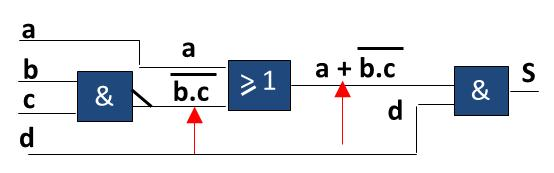
\includegraphics[width=3.04651in,height=0.95135in]{14-Logique/Cours/pandoc/media/image29.jpeg}

Pour une réalisation «~câblée~», il faut alors disposer de tous les circuits logiques.
\end{quote}

Plus on aura de diversité et plus le circuit sera complexe. \textbf{Elle n'est utilisée que dans des cas simples}.

\begin{longtable}[]{@{}
  >{\raggedright\arraybackslash}p{(\columnwidth - 2\tabcolsep) * \real{0.1250}}
  >{\raggedright\arraybackslash}p{(\columnwidth - 2\tabcolsep) * \real{0.8611}}@{}}
\toprule\noalign{}
\begin{minipage}[b]{\linewidth}\raggedright
\begin{quote}
{[}{]} (14-Lo gique/ Cours/ pandoc /media /image 10.png )\{widt h=``0.6 262696 850393 701in''

height =``0.65 083333 333333 34in''\}
\end{quote}
\end{minipage} & \begin{minipage}[b]{\linewidth}\raggedright
\textbf{Equations logiques}

\textbf{Donner les équations des sorties S1, S2 et S3.}

\begin{center}

\includegraphics[width=3.20833in,height=3.27626in]{14-Logique/C ours/pandoc/media/image30.png}

exo1
\end{center}
\end{minipage} \\
\midrule\noalign{}
\endhead
\bottomrule\noalign{}
\endlastfoot
& \\
\end{longtable}

\hypertarget{synthuxe8se-par-circuits-programmables}{%
\subparagraph*{Synthèse par circuits programmables}\label{synthuxe8se-par-circuits-programmables}}
\addcontentsline{toc}{subparagraph}{Synthèse par circuits programmables}

Les circuits logiques programmables appelés PLD se répartissent en différentes familles et sont des solutions de plus en plus utilisées. On distingue principalement deux types de familles :

\begin{itemize}
\item
  Les \textbf{circuits ASIC} (Application Specific Integrated Circuit), sont des circuits qui ne sont pas reconfigurables et qui sont prévus pour des applications spécifiques (téléphone portable,\ldots);
\item
  Les \textbf{circuits PLD} (Programmable Logic Device), sont des circuits avec ds associations de blocs combinatoires configurables par l'utilisateur. Il y a alors plusieurs familles suivant les besoins.

  \begin{itemize}
  \item
    Les \textbf{FPGA} (Field Programmable Gate Array),
  \item
    Les \textbf{PAL} (Programmable Array Logic),
  \item
    Les \textbf{GAL} (Generic Array Logic),
  \item
    Les \textbf{CPLD} (Programmable Logic Device)
  \end{itemize}
\end{itemize}

\hypertarget{fonctions-combinatoires-particuliuxe8res}{%
\subsubsection{Fonctions combinatoires particulières}\label{fonctions-combinatoires-particuliuxe8res}}

\hypertarget{codeur-duxe9codeur-et-transcodeur}{%
\subparagraph*{Codeur, Décodeur et Transcodeur}\label{codeur-duxe9codeur-et-transcodeur}}
\addcontentsline{toc}{subparagraph}{Codeur, Décodeur et Transcodeur}

Dans un \textbf{système combinatoire} complexe, on utilisera un «~cerveau~» ou calculateur qui permet de traiter les informations d'entrées et de définir les sorties en conséquence.

Par exemple, si on souhaite réaliser le circuit d'affichage d'un code tapé au clavier, on aura la structure suivante.

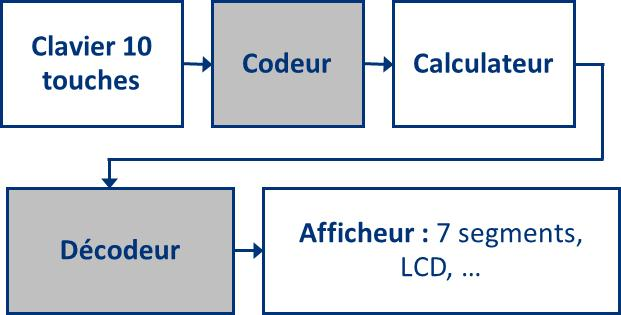
\includegraphics[width=2.77907in,height=1.40967in]{14-Logique/Cours/pandoc/media/image31.jpeg}

Deux interfaces, appelées \textbf{codeur et décodeur}, ont été ajoutées afin de permettre la «~\textbf{communication}~» entre le clavier, le calculateur et l'afficheur. En effet, chacun à un code propre qui n'est pas forcément compris par tout le monde. Le \textbf{codeur} permet de \textbf{transcrire un code quelconque en des informations binaires exploitables par le calculateur}. C'est un circuit combinatoire comportant n entrées (une seule entrée est active à la fois) et p sorties.

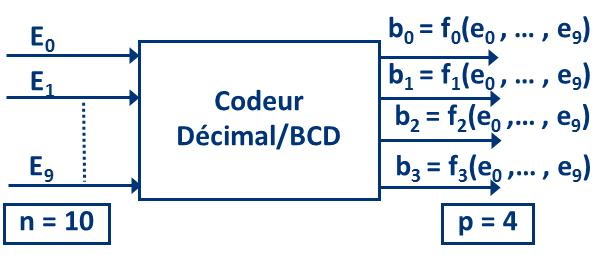
\includegraphics[width=3.19767in,height=1.34722in]{14-Logique/Cours/pandoc/media/image32.jpeg}

Le \textbf{décodeur} permet de réaliser l'opération inverse du codeur. Il permet de transcrire des informations binaires fournies par le calculateur en un code quelconque.

C'est un circuit combinatoire comportant n entrées et p = 2\textsuperscript{n} sorties.

A une combinaison d'entrées, il ne correspond \ul{qu'une seule sortie active.}

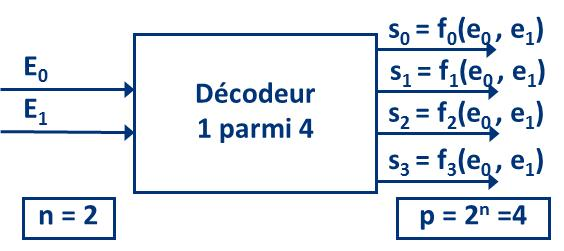
\includegraphics[width=2.9786in,height=1.32558in]{14-Logique/Cours/pandoc/media/image33.jpeg}

Un \textbf{transcodeur} est un circuit combinatoire comportant n entrées et p sorties. C'est un \textbf{« convertisseur de code ».} Le plus connu est le transcodeur Gray/Binaire ou le BCD/7 segments pour l'affichage. L'afficheur 7 segments permet, à partir de 7 LEDs d'afficher tous les chiffres décimaux comme sur la figure suivante.

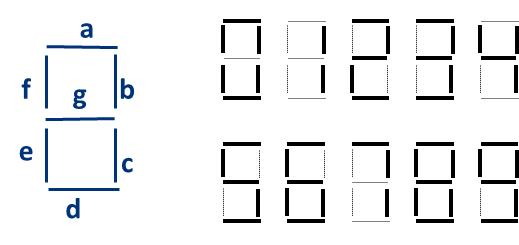
\includegraphics[width=2.52326in,height=1.19113in]{14-Logique/Cours/pandoc/media/image34.jpeg}

\textbf{\ul{Table de vérité du décodeur 7 segments :}}

\begin{longtable}[]{@{}
  >{\raggedright\arraybackslash}p{(\columnwidth - 30\tabcolsep) * \real{0.0556}}
  >{\raggedright\arraybackslash}p{(\columnwidth - 30\tabcolsep) * \real{0.0278}}
  >{\raggedright\arraybackslash}p{(\columnwidth - 30\tabcolsep) * \real{0.1111}}
  >{\raggedright\arraybackslash}p{(\columnwidth - 30\tabcolsep) * \real{0.0764}}
  >{\raggedright\arraybackslash}p{(\columnwidth - 30\tabcolsep) * \real{0.0764}}
  >{\raggedright\arraybackslash}p{(\columnwidth - 30\tabcolsep) * \real{0.0764}}
  >{\raggedright\arraybackslash}p{(\columnwidth - 30\tabcolsep) * \real{0.0208}}
  >{\raggedright\arraybackslash}p{(\columnwidth - 30\tabcolsep) * \real{0.0417}}
  >{\raggedright\arraybackslash}p{(\columnwidth - 30\tabcolsep) * \real{0.1111}}
  >{\raggedright\arraybackslash}p{(\columnwidth - 30\tabcolsep) * \real{0.0556}}
  >{\raggedright\arraybackslash}p{(\columnwidth - 30\tabcolsep) * \real{0.0556}}
  >{\raggedright\arraybackslash}p{(\columnwidth - 30\tabcolsep) * \real{0.0556}}
  >{\raggedright\arraybackslash}p{(\columnwidth - 30\tabcolsep) * \real{0.0556}}
  >{\raggedright\arraybackslash}p{(\columnwidth - 30\tabcolsep) * \real{0.0556}}
  >{\raggedright\arraybackslash}p{(\columnwidth - 30\tabcolsep) * \real{0.0556}}
  >{\raggedright\arraybackslash}p{(\columnwidth - 30\tabcolsep) * \real{0.0556}}@{}}
\toprule\noalign{}
\endhead
\bottomrule\noalign{}
\endlastfoot
& & \textbf{Sorties du Calculateur} & & & & & & \textbf{Segments de l'afficheur} & & & & & & & \\
\textbf{N} & & \textbf{a\textsubscript{3}} & \textbf{a\textsubscript{2}} & \textbf{a\textsubscript{1}} & \textbf{a\textsubscript{0}} & & & & \textbf{a} & \textbf{b} & \textbf{c} & \textbf{d} & \textbf{e} & \textbf{f} & \textbf{g} \\
\textbf{0} & & 0 & 0 & 0 & 0 & & & & 1 & 1 & 1 & 1 & 1 & 1 & 0 \\
\textbf{1} & & 0 & 0 & 0 & 1 & & & & 0 & 1 & 1 & 0 & 0 & 0 & 0 \\
\textbf{2} & & 0 & 0 & 1 & 0 & & & & 1 & 1 & 0 & 1 & 1 & 0 & 1 \\
\textbf{3} & & 0 & 0 & 1 & 1 & & & & 1 & 1 & 1 & 1 & 0 & 0 & 1 \\
\textbf{4} & & 0 & 1 & 0 & 0 & & & & 0 & 1 & 1 & 0 & 0 & 1 & 1 \\
\textbf{5} & & 0 & 1 & 0 & 1 & & & & 1 & 0 & 1 & 1 & 0 & 1 & 1 \\
\textbf{6} & & 0 & 1 & 1 & 0 & & & & 1 & 0 & 1 & 1 & 1 & 1 & 1 \\
\textbf{7} & & 0 & 1 & 1 & 1 & & & & 1 & 1 & 1 & 0 & 0 & 0 & 0 \\
\textbf{8} & & 1 & 0 & 0 & 0 & & & & 1 & 1 & 1 & 1 & 1 & 1 & 1 \\
\textbf{9} & & 1 & 0 & 0 & 1 & & & & 1 & 1 & 1 & 1 & 0 & 1 & 1 \\
\end{longtable}

\textbf{L'équation logique de la sortie} peut alors être déterminée en recherchant toutes les \textbf{combinaisons d'entrées pour lesquelles la sortie vaut 1.}

\begin{quote}
Le \textbf{code Gray (ou binaire réfléchi)}, également appelé binaire réfléchi, est un code \textbf{binaire} qui présente la particularité qu\textquotesingle{}\textbf{un seul bit change d\textquotesingle état entre deux combinaisons successives}.

Ce qui permet d\textquotesingle éviter des erreurs de lecture.
\end{quote}

\begin{longtable}[]{@{}
  >{\raggedright\arraybackslash}p{(\columnwidth - 2\tabcolsep) * \real{0.5000}}
  >{\raggedright\arraybackslash}p{(\columnwidth - 2\tabcolsep) * \real{0.5000}}@{}}
\toprule\noalign{}
\begin{minipage}[b]{\linewidth}\raggedright
\hypertarget{code-bi}{%
\subparagraph{Code bi}\label{code-bi}}

naire \{\#code-binaire .unnumbered\}

\hypertarget{section}{%
\subsection{----------}\label{section}}

\[2^{2}\] \[2^{1}\] \[2^{0}\] ------- -- --------- ----------- -----------

0 0 0 0

1 0 0 1

2 0 1 0

3 0 1 1

4 1 0 0

5 1 0 1

6 1 1 0

7 1 1 1 ---------- ---------------------------------
\end{minipage} & \begin{minipage}[b]{\linewidth}\raggedright
\hypertarget{c}{%
\subparagraph{C}\label{c}}

ode Gray \{\#code-gray .unnumbered\}

\hypertarget{section-1}{%
\subsection{----------}\label{section-1}}

\[2^{2}\] \[2^{1}\] \[2^{0}\] ------- -- --------- ----------- -----------

0 0 0 0

1 0 0 1

2 0 1 1

3 0 1 0

4 1 1 0

5 1 1 1

6 1 0 1

7 1 0 0 ---------- ---------------------------------
\end{minipage} \\
\midrule\noalign{}
\endhead
\bottomrule\noalign{}
\endlastfoot
& \\
\end{longtable}

\begin{longtable}[]{@{}
  >{\raggedright\arraybackslash}p{(\columnwidth - 2\tabcolsep) * \real{0.1250}}
  >{\raggedright\arraybackslash}p{(\columnwidth - 2\tabcolsep) * \real{0.8611}}@{}}
\toprule\noalign{}
\begin{minipage}[b]{\linewidth}\raggedright
\begin{quote}
{[}{]} (14-Lo gique/ Cours/ pandoc /media /image 10.png )\{widt h=``0.6 262696 850393 701in''

height =``0.65 083333 333333 34in''\}
\end{quote}
\end{minipage} & \begin{minipage}[b]{\linewidth}\raggedright

\includegraphics[width=1.13542in,height=0.95833in]{14-Logique/Co urs/pandoc/media/image35.jpeg}\textbf{Conditionneuse de comprimés pharmaceutiques}

Une unité de conditionnement de médicaments permet de mettre en flacon une quantité préréglée de comprimés de façon automatique.

Ces comprimés sont déversés sur un plateau tournant entraîné par une machine à courant continu. Le débit des comprimés sortant de la trémie est contrôlé par une trappe. Le débit est réglable de façon à maintenir un nombre de comprimés suffisant sur la sole par ouverture ou fermeture d'une trappe (par l'intermédiaire de 2 boutons poussoirs à bascule). La trappe est actionnée par un vérin électrique VE.

\begin{center}

\includegraphics[width=3.4375in,height=1.65625in]{1 4-Logique/Cours/pandoc/media/image36.jpeg}

api
\end{center}

Le conditionnement de comprimés délivre une information numérique sur un mot de 8 bits, soit un octet A = {[}a7 a6 a5 \ldots{} a0{]} correspondant à la position souhaitée du vérin.

La course totale du vérin est de 50 mm. Le pas de la vis est de 1mm.

Le code GRAY fourni par le codeur présente l'inconvénient de ne pas permettre de manière simple les opérations arithmétiques de base et notamment la comparaison entre les nombres qui le composent. On envisage de concevoir un circuit combinatoire (appelé transcodeur) permettant de passer du code GRAY au code binaire naturel, et ainsi de fournir une information directement exploitable par l'automate.

\begin{center}

\includegraphics[width=5.33333in,height=0.89583in]{14-Logique/C ours/pandoc/media/image37.jpeg}

qsd
\end{center}

\textbf{Déterminer la résolution du codeur rotatif 8 bits en degrés puis en mm.}

\textbf{Etablir les équations logiques des sorties B1 à B4 du transcodeur en fonction des entrées G1 à G4.}

\textbf{En déduire l'expression logique liant le bit Bi en fonction du bit Bi+1 et du bit Gi pour n bits.}

\textbf{Dessiner le logigramme complet du transcodeur 4 bits en utilisant les opérateurs logiques élémentaires notamment l'opérateur OU EXCLUSIF.}
\end{minipage} \\
\midrule\noalign{}
\endhead
\bottomrule\noalign{}
\endlastfoot
& \\
\end{longtable}

\hypertarget{multiplexeur-duxe9multiplexeur}{%
\subparagraph*{Multiplexeur / Démultiplexeur}\label{multiplexeur-duxe9multiplexeur}}
\addcontentsline{toc}{subparagraph}{Multiplexeur / Démultiplexeur}

Un \textbf{multiplexeur} est un «~aiguilleur~» d'information. On sélectionne l'information à envoyer en sortie à partir \textbf{d'entrées de sélections}. Un multiplexeur est donc un système combinatoire comportant N entrées de données et une sortie qui permet de transmettre les informations présentent en entrée suivant les n entrées de sélection (N = 2\textsuperscript{n}).

Il existe souvent une \textbf{entrée dite de «~validation}~\textbf{»} (ou enable en anglais) qui permet de valider le fonctionnement du Mux. Si le Mux n'est pas validé, la sortie sera toujours nulle. Cette entrée est généralement active à l'état bas (d'où la présence du petit triangle sur l'entrée).

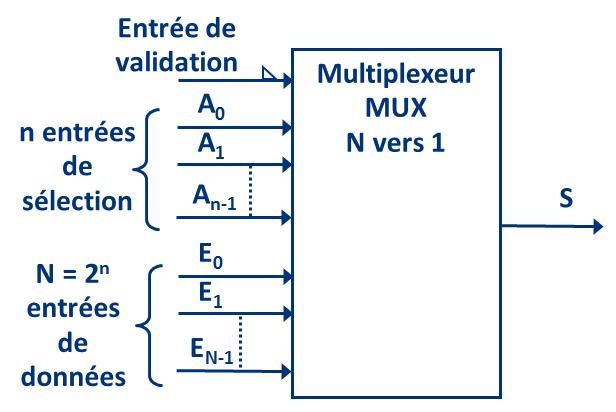
\includegraphics[width=2.86047in,height=1.91317in]{14-Logique/Cours/pandoc/media/image38.jpeg}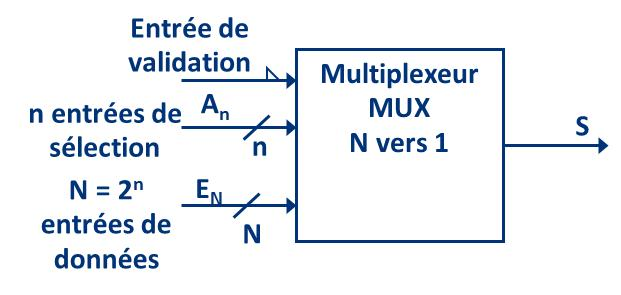
\includegraphics[width=2.81395in,height=1.33674in]{14-Logique/Cours/pandoc/media/image39.jpeg}

Par exemple, pour un MUX 8 vers 1, il suffit d'avoir 3 entrées de sélections. La table de vérité du fonctionnement est la suivante.

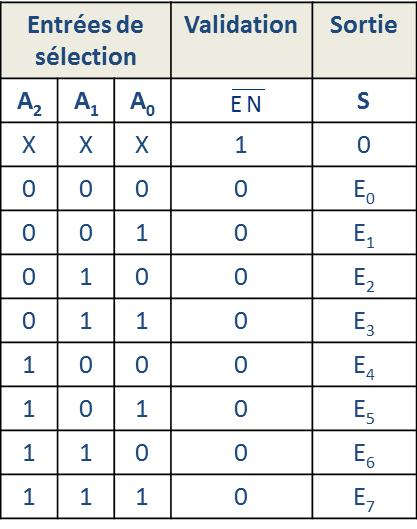
\includegraphics[width=2.09902in,height=2.66279in]{14-Logique/Cours/pandoc/media/image40.jpeg}

Un \textbf{démultiplexeur} réalise l'opération inverse d'un multiplexeur en aiguillant une donnée d'entrée vers une des 2n sorties choisie par les n entrées de sélection. Les applications des multiplexeurs / démultiplexeurs sont diverses~ : synthèse d'une fonction logique, multiplexage d'un système combinatoire (afin de limiter la complexité et les coûts, conversion série/parallèle et la génération de fonctions (GBF).

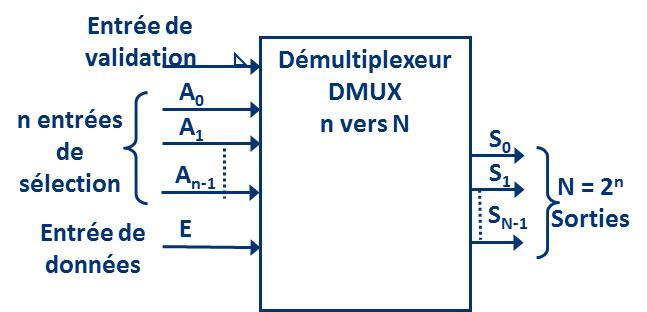
\includegraphics[width=3.18292in,height=1.53488in]{14-Logique/Cours/pandoc/media/image41.jpeg}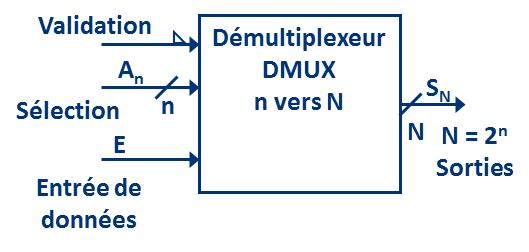
\includegraphics[width=2.53488in,height=1.20754in]{14-Logique/Cours/pandoc/media/image42.jpeg}

\textbf{Synthèse à base de multiplexeur :}

Le \textbf{multiplexeur} permet de «~découper~» la table de vérité et ainsi de \textbf{sélectionner en sortie l'une des 2n entrées}. Il suffit alors de mettre les entrées comme sélecteur et de «~recopier~» la table de vérité sur les entrées de données.

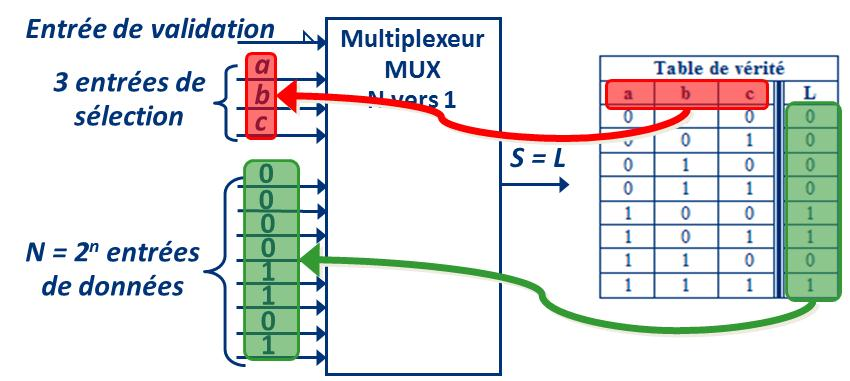
\includegraphics[width=4.43023in,height=1.98579in]{14-Logique/Cours/pandoc/media/image43.jpeg}

\hypertarget{technologie-des-circuits-intuxe9gruxe9s}{%
\subsubsection{Technologie des circuits intégrés}\label{technologie-des-circuits-intuxe9gruxe9s}}

\hypertarget{familles-technologiques}{%
\subparagraph*{Familles technologiques}\label{familles-technologiques}}
\addcontentsline{toc}{subparagraph}{Familles technologiques}

Pour synthétiser une fonction logique, on peut utiliser des \textbf{circuits intégrés logiques} qui sont classés suivant leur \textbf{technologie de fabrication} \textbf{(TTL, CMOS, ECL,\ldots).} Les différents critères (électriques et temporels) permettant de comparer les performances d'une famille technologique sont~:

\begin{itemize}
\item
  Les \textbf{tensions d'alimentations} ;
\item
  Les \textbf{niveaux de tensions associés aux niveaux logiques} (pour quelle tension on aura un «~0~» ou un «~1~»);
\item
  Les \textbf{courants maximums d'entrée et de sortie} ;
\item
  La \textbf{puissance maximale consommée} ;
\item
  Le \textbf{temps de propagation} et les temps de montée et de descente.
\end{itemize}

Chaque technologie aura alors ses points forts et ses points faibles et on choisira la technologie suivant l'application souhaitée.

\hypertarget{niveaux-de-tension}{%
\subparagraph*{Niveaux de tension}\label{niveaux-de-tension}}
\addcontentsline{toc}{subparagraph}{Niveaux de tension}

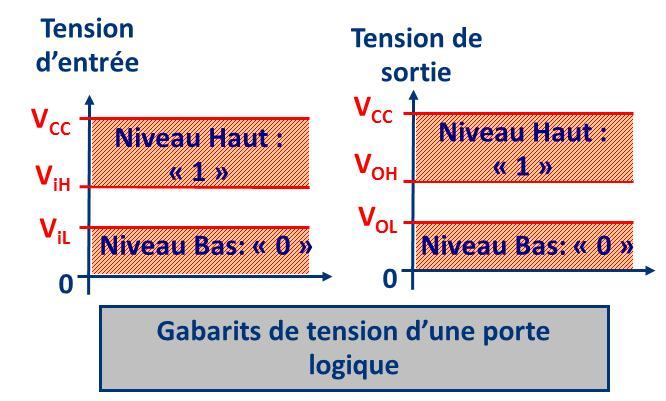
\includegraphics[width=3.0814in,height=1.85531in]{14-Logique/Cours/pandoc/media/image44.jpeg}Les circuits logiques sont alimentés entre deux tensions~: \textbf{0V (ou VSS ou GND)} et \textbf{+Vcc (ou VDD).}

Dans les circuits intégrés logiques, on a une tension qui est associée à chaque niveau logique (0 ou 1).

Le \textbf{«~1~»} correspond alors au potentiel le plus élevé (\textbf{H comme High}) et le \textbf{«~0~»} comme le potentiel le plus bas (\textbf{L comme Low}).

\hypertarget{temps-de-propagation}{%
\subparagraph*{\texorpdfstring{\protect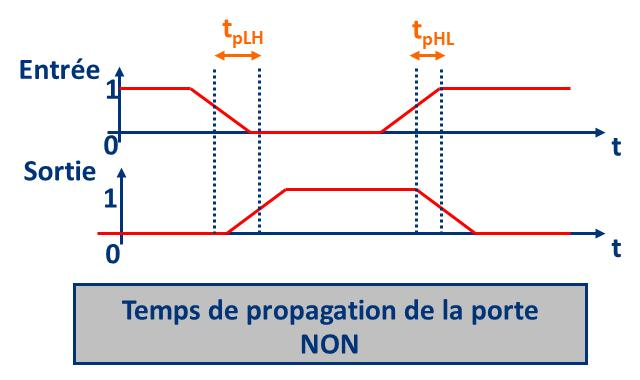
\includegraphics[width=2.99444in,height=1.77778in]{14-Logique/Cours/pandoc/media/image45.jpeg}Temps de propagation}{Temps de propagation}}\label{temps-de-propagation}}
\addcontentsline{toc}{subparagraph}{Temps de propagation}

Le \textbf{temps de propagation d'une porte} est le \textbf{temps (ou retard) que met l'information à apparaître en sortie}. Ce temps de propagation est \textbf{dû à deux choses}~: le \textbf{temps de propagation à travers le circuit électronique} et la \textbf{durée nécessaire à l'évolution de la sortie}. Par exemple on peut voir les temps de propagations d'une porte NON :

\hypertarget{sortance-fan-out}{%
\subparagraph*{Sortance (fan out)}\label{sortance-fan-out}}
\addcontentsline{toc}{subparagraph}{Sortance (fan out)}

La sortance est le \textbf{nombre d'entrées que peut piloter une porte logique}. Dans le cas où la sortance n'est pas suffisante, on utilise des circuits «~bufferisés~» qui permettent d'augmenter le courant disponible en sortie (on a un montage Darlington sur les transistors de sortie). Les circuits à sortie bufférisé sont repérés par le symbole amplification~

\hypertarget{consommation}{%
\subparagraph*{Consommation}\label{consommation}}
\addcontentsline{toc}{subparagraph}{Consommation}

La puissance consommée dépend du courant total consommé (nombre de portes utilisées) pour la technologie TTL mais aussi de la fréquence pour la technologie CMOS. Pour des fréquences élevées, la puissance consommée par les technologies TTL est aussi fonction de la fréquence.

\hypertarget{ruxe9sistances-de-rappel-pull-up-pull-down}{%
\subparagraph*{Résistances de rappel (Pull-up, Pull-down)}\label{ruxe9sistances-de-rappel-pull-up-pull-down}}
\addcontentsline{toc}{subparagraph}{Résistances de rappel (Pull-up, Pull-down)}

En électronique numérique il faut faire extrêmement attention aux \textbf{tensions appliquées aux entrées des portes logiques}.

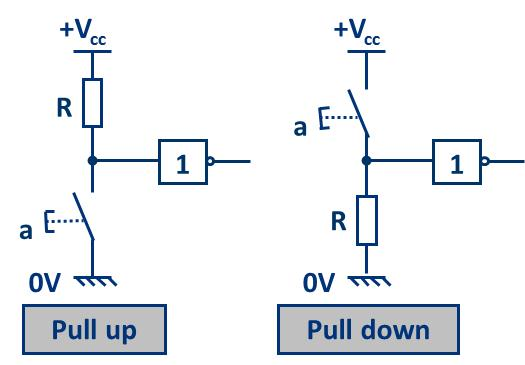
\includegraphics[width=2.7093in,height=1.88361in]{14-Logique/Cours/pandoc/media/image46.jpeg}En effet, si les \textbf{potentiels ne sont pas imposés sur toutes les entrées} (entrée non connectée par exemple), son état est \textbf{indéterminé et peut prendre la valeur «~0~» ou «~1~» suivant le gabarit de tension}.

Pour fixer les potentiels, on ajoute ce qu'on appelle les \textbf{résistances de tirages ou pull-up}. Une résistance de tirage permet d'imposer un potentiel sur une entrée logique. On parle de pull-up, lorsque la résistance est reliée au +Vcc et de pull-down lorsqu'elle est reliée à la masse.

Dans l'exemple du pull up ci-dessus, la résistance permet d'avoir un potentiel de référence (+Vcc), lorsque le bouton poussoir «~a~» n'est pas actionné. Elle évite ainsi d'avoir des potentiels flottants.

\hypertarget{sortie-standard}{%
\subparagraph*{Sortie standard}\label{sortie-standard}}
\addcontentsline{toc}{subparagraph}{Sortie standard}

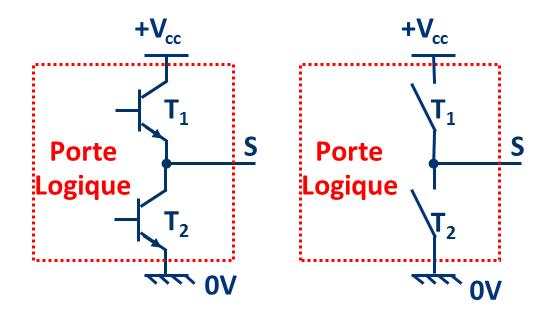
\includegraphics[width=2.78542in,height=1.67222in]{14-Logique/Cours/pandoc/media/image47.jpeg} La sortie de portes logiques «\textbf{~standards}~» peut-être vue comme deux transistors T1 et T2 qui sont tour à tour bloqué ou saturé de manière complémentaire. On a alors deux états possibles en sortie «~0~» ou «~1~», comme le montre les figures suivantes.

Le principal inconvénient de la sortie standard est \textbf{qu'on ne peut pas relier plusieurs portes sur un même bus} car on risque d'avoir un conflit (deux circuits peuvent très bien imposer un niveau différent alors qu'un seul est utilisé).

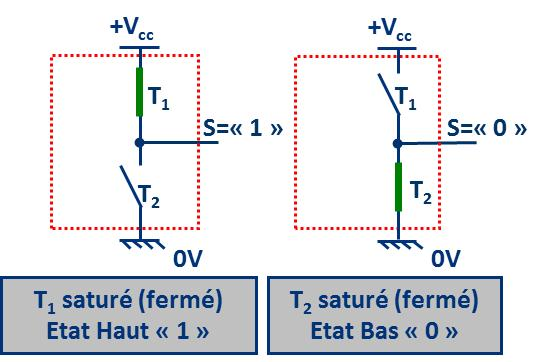
\includegraphics[width=2.69767in,height=1.79185in]{14-Logique/Cours/pandoc/media/image48.jpeg}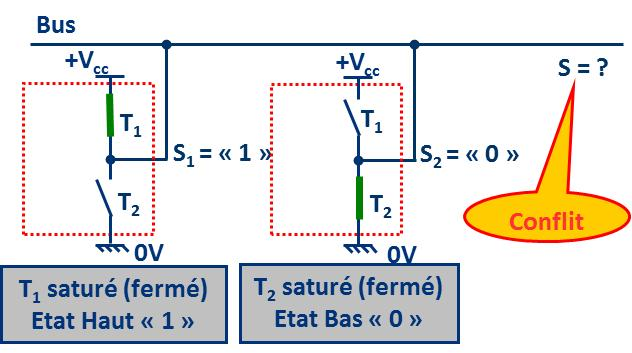
\includegraphics[width=2.93023in,height=1.63666in]{14-Logique/Cours/pandoc/media/image49.jpeg}

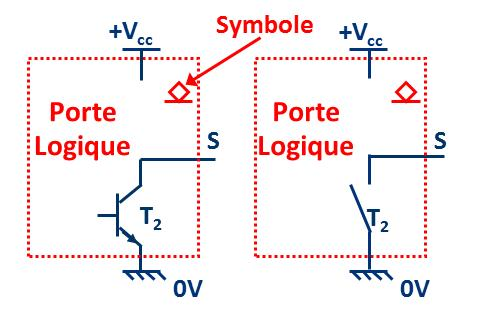
\includegraphics[width=2.34483in,height=1.53132in]{14-Logique/Cours/pandoc/media/image50.jpeg}

\hypertarget{sortie-collecteur-ouvert}{%
\subparagraph*{Sortie « collecteur ouvert »}\label{sortie-collecteur-ouvert}}
\addcontentsline{toc}{subparagraph}{Sortie « collecteur ouvert »}

Les portes ayant une sortie à \textbf{collecteur ouvert} ont une sortie avec un seul transistor, dont le collecteur est relié à la sortie (collecteur «~ouvert~»). Cette sortie est représentée sur les figures ci-dessous.

Cette structure n'a aucun problème pour imposer le niveau bas ou «~0~», mais \textbf{ne peut imposer le niveau haut} ou «~1~». Pour «~l'aider~» à imposer ce niveau haut, il \textbf{faut alors une résistance de pull-up}, qui n'interférera pas sur le niveau bas comme le montre la figure suivante.

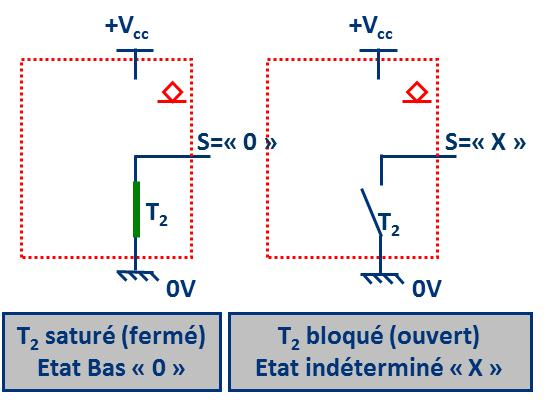
\includegraphics[width=2.65674in,height=1.95349in]{14-Logique/Cours/pandoc/media/image51.jpeg}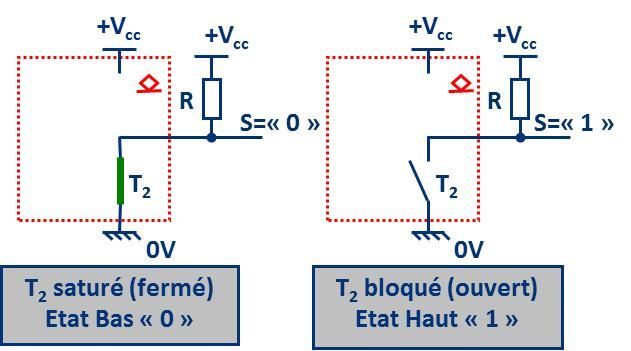
\includegraphics[width=3.29086in,height=1.83058in]{14-Logique/Cours/pandoc/media/image52.jpeg}

\hypertarget{sortie-3-uxe9tats}{%
\subparagraph*{Sortie « 3 états »}\label{sortie-3-uxe9tats}}
\addcontentsline{toc}{subparagraph}{Sortie « 3 états »}

Les circuits logiques à sortie \textbf{«~3 états~»} utilisent comme la sortie standard deux transistors. Cependant, il existe dans ces circuits une \textbf{entrée supplémentaire dite de validation (ou Enable en anglais)} qui permet de «~déconnecter~» le circuit d'un bus et ainsi d'éviter les conflits.

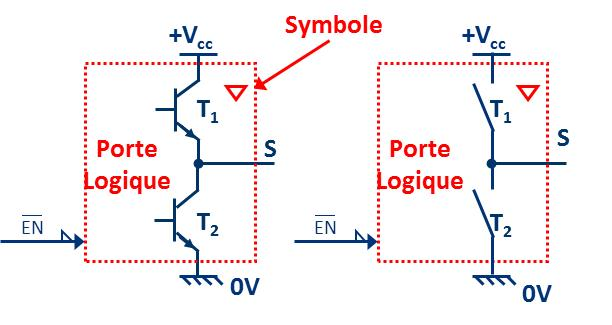
\includegraphics[width=3.46552in,height=1.84035in]{14-Logique/Cours/pandoc/media/image53.jpeg}

En effet, lorsque l'entrée de validation n'est pas active, on retrouve le fonctionnement standard avec deux états possibles «~0~» ou «~1~».

Cependant, lorsqu'on n'utilise plus le circuit, on peut le désactiver via l'entrée de validation. Les deux transistors sont alors bloqués et on n'impose aucun niveau logique en sortie comme l'illustre les figures suivantes.

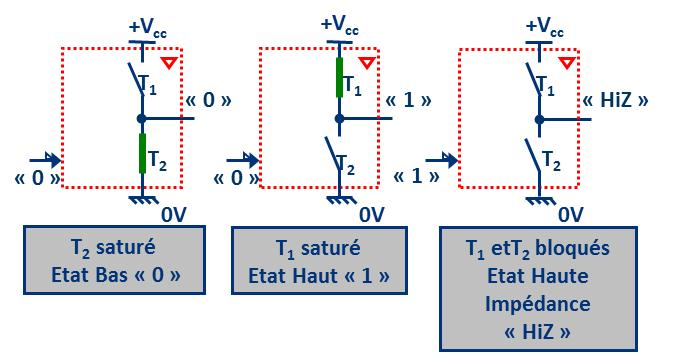
\includegraphics[width=3.90698in,height=2.08064in]{14-Logique/Cours/pandoc/media/image54.jpeg}

On définit alors un troisième état qui est l'état \textbf{Haute Impédance ou HiZ}. On peut alors connecter plusieurs circuits sur un même bus sans risque de conflit s'ils sont actifs chacun leur tour. Ces sorties sont notamment utilisées pour les mémoires (bus d'adresses et bus de données).

\hypertarget{systuxe8mes-uxe0-uxe9vuxe8nements-discrets-sed}{%
\subsection{Systèmes à évènements Discrets (SED)}\label{systuxe8mes-uxe0-uxe9vuxe8nements-discrets-sed}}

\hypertarget{exemple-introductif}{%
\subsubsection{Exemple introductif}\label{exemple-introductif}}

On souhaite réaliser la commande d'un moteur d'ouverture du hayon \textbf{M+} à partir des différentes entrées logiques du système :

\begin{itemize}
\item
  \textbf{ph = 1} si le coffre est en position haute (coffre ouvert);
\item
  \textbf{t0 = 1}; si une pression est exercée sur l'une des touches \textgreater{} d'ouverture automatique ;
\end{itemize}

Le chronogramme du fonctionnement souhaité est le suivant : Lorsqu'on appuie sur la commande d'ouverture (t0) le hayon s'ouvre (M+) jusqu'à atteindre la position haute (ph).

Pour trouver la table de vérité de ce système il suffit d'étudier les différents cas du chronogramme. Un système combinatoire de 2 entrées a 4 possibilités.

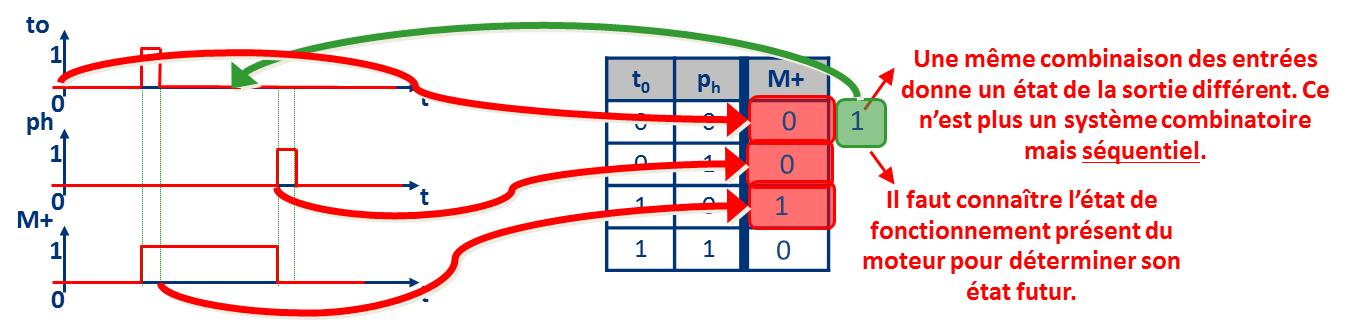
\includegraphics[width=6.83716in,height=1.67513in]{14-Logique/Cours/pandoc/media/image55.jpeg}

Pour trouver la table de vérité de ce système il suffit alors de rajouter une entrée qui représente l'état présent du moteur M+.

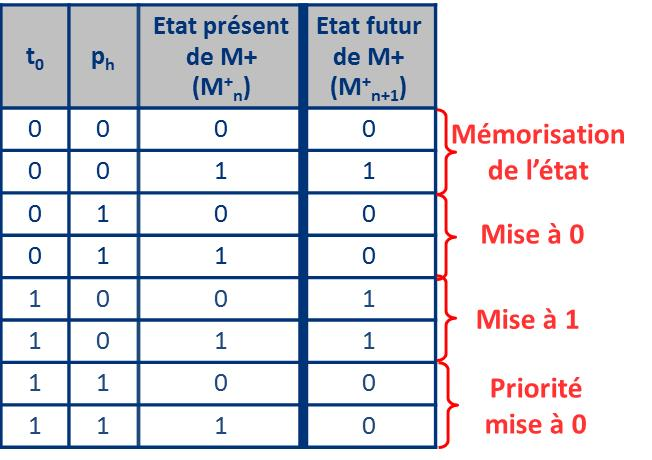
\includegraphics[width=2.87662in,height=2.02951in]{14-Logique/Cours/pandoc/media/image56.jpeg}

\[{M^{+}}_{n + 1} = \overline{to}.\overline{ph}.{M^{+}}_{n} + to.\overline{ph}.\overline{{M^{+}}_{n}} + to.\overline{ph}.{M^{+}}_{n} = to.\overline{ph} + \overline{to}.\overline{ph}.{M^{+}}_{n} = to.\overline{ph} + \overline{ph}.{M^{+}}_{n}\]

L'équation logique de la sortie est alors : \({M^{+}}_{n + 1} = to.\overline{ph} + \overline{ph}.{M^{+}}_{n} = \overline{ph}.\left( to + {M^{+}}_{n} \right)\)

Cette équation logique peut être représentée par un logigramme.

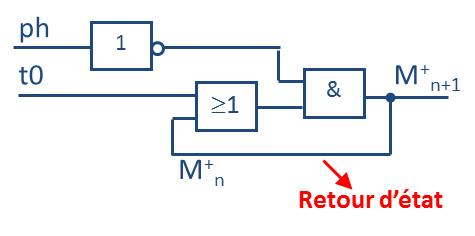
\includegraphics[width=2.36902in,height=1.17703in]{14-Logique/Cours/pandoc/media/image57.jpeg}

La différence par rapport aux logigrammes de circuits combinatoires est le \textbf{retour d'état} de la sortie du système comme entrée. Pour cela, il faut \textbf{mémoriser l'état du système}.

\hypertarget{systuxe8mes-suxe9quentiels}{%
\subsubsection{Systèmes séquentiels}\label{systuxe8mes-suxe9quentiels}}

Nous avons vu les systèmes combinatoires pour lesquels \textbf{à un état des entrées correspondait un unique état des sorties}. Il existait alors une table de correspondance entre entrées et sorties qu'on appelait \textbf{table de vérité.} Dans les systèmes séquentiels, les états des sorties ne dépendent plus uniquement des entrées du système \textbf{mais aussi des événements antérieurs.}

\textbf{Une même combinaison des entrées, à un certain instant, ne donne pas toujours la même sortie} mais dépend aussi de l'état précédent de cette dernière. C'est l'«~\textbf{effet mémoire}~» qui utilise la notion \textbf{d'état interne du système.}

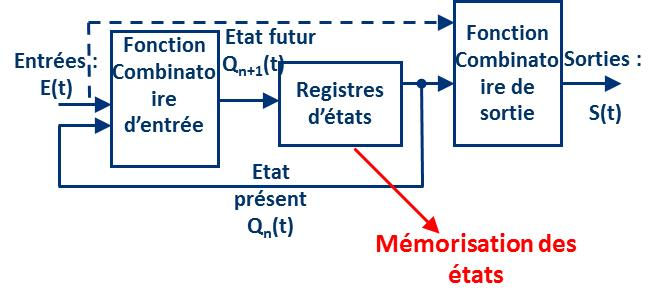
\includegraphics[width=3.41597in,height=1.59028in]{14-Logique/Cours/pandoc/media/image58.jpeg}Ce dernier sera stable, tant qu'aucune combinaison des entrées n'aura fait changer d'état. \textbf{Les états des sorties dépendent donc des états des entrées mais aussi de} \textbf{l'état interne antérieur du système}. On peut représenter un système séquentiel à partir d'un système combinatoire à partir du schéma suivant où on mémorise l'état interne du système.

Pour décrire les systèmes séquentiels, on n'utilise donc plus la table de vérité mais ce qu'on appelle une \textbf{table des états} où on prend en compte l'état interne du système qui est ajouté comme variable d'entrée. Pour trouver \textbf{l'état futur} (Q\textsubscript{n+1}), on utilise \textbf{l'état présent} du système (Q\textsubscript{n}).

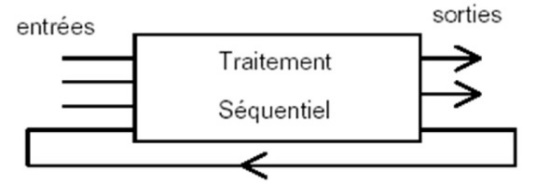
\includegraphics[width=2.43472in,height=0.83611in]{14-Logique/Cours/pandoc/media/image59.jpeg}

Un système est dit à logique séquentielle, lorsque la ou les sorties \textbf{dépendent de la combinaison des entrées mais aussi de l\textquotesingle état précédent des sorties et de la variable temps.}

\ul{Explication :} Une même cause (même combinaison des entrées e\textsubscript{1}, e\textsubscript{2}, \ldots, e \textsubscript{n}) peut produire des effets différents (états différents des sorties S\textsubscript{1}, S\textsubscript{2}, \ldots, S \textsubscript{p}). L\textquotesingle effet peut persister si la cause disparaît. S\textsubscript{i}= f(e\textsubscript{1},e\textsubscript{2},\ldots,e \textsubscript{n}; S\textsubscript{1},S\textsubscript{2},...,S\textsubscript{p}; t)

\textbf{Comment décrire le comportement séquentiel d'un système ?}

La description du comportement d'un système séquentiel peut être réalisée notamment par :

\begin{itemize}
\item
  L'outil graphe d'états ;
\item
  L'outil algorithme (ou algorigramme).
\end{itemize}

Il s'agit essentiellement d'outils graphiques permettant de modéliser le comportement séquentiel en termes de déroulement d'actions temporelles. Ces outils sont, à la base, des outils de modélisation du comportement séquentiel, mais peuvent aussi servir à la programmation des composants réalisant la fonction Traiter de la chaîne d'information (microcontrôleur, microprocesseur, automate programmable, \ldots).

Les variables d'entrées de la fonction Traiter sont alors les grandeurs fournies par la fonction Acquérir (capteurs, \ldots) et les variables de sorties sont les informations destinées à la fonction Communiquer, qui permettront d'élaborer les ordres à la chaîne d'énergie

Quel que soit l'outil adopté pour modéliser le comportement séquentiel d'un système, il existe souvent plusieurs « solutions ». « La solution » la plus simple et celle qui respecte l'ensemble des contraintes est donc à privilégier. C'est le rôle de l'ingénieur de choisir le « bon » outil, et la « meilleure solution~».

Les systèmes à événements discrets (SED) se définissent par opposition aux systèmes continus dont l\textquotesingle évolution est continue dans le temps et peut être décrite par des équations différentielles. Dans un SED, le passage d'un état à un autre est déclenché par des événements ponctuels. Contrairement aux systèmes continus où les informations traitées sont de nature analogique, les systèmes à événements discrets manipulent des informations logiques ou numériques.

\hypertarget{diagramme-duxe9tat-stm}{%
\subsubsection{Diagramme d'état~(stm)}\label{diagramme-duxe9tat-stm}}

\hypertarget{pruxe9sentation}{%
\subparagraph*{Présentation}\label{pruxe9sentation}}
\addcontentsline{toc}{subparagraph}{Présentation}

En langage SysML, un diagramme d'état (stm) est nécessairement associé à un bloc du diagramme de définitions de blocs (bdd) ou du diagramme de blocs internes (ibd). Ce bloc peut être le système, un sous-système ou un composant.

\begin{quote}
Le \textbf{diagramme d'état} représente le \textbf{comportement} du système et ses changements d'état en fonction des interactions.
\end{quote}

\begin{longtable}[]{@{}
  >{\raggedright\arraybackslash}p{(\columnwidth - 2\tabcolsep) * \real{0.1250}}
  >{\raggedright\arraybackslash}p{(\columnwidth - 2\tabcolsep) * \real{0.8611}}@{}}
\toprule\noalign{}
\begin{minipage}[b]{\linewidth}\raggedright
\begin{quote}
{[}{]} (14-Lo gique/ Cours/ pandoc /media /image 10.png )\{widt h=``0.6 262696 850393 701in''

height =``0.65 083333 333333 34in''\}
\end{quote}
\end{minipage} & \begin{minipage}[b]{\linewidth}\raggedright

\includegraphics[width=1.86458in,height=1.65347in]{14-Logique/Co urs/pandoc/media/image60.jpeg}\textbf{Vidéo Surveillance}

Le diagramme ci-dessous décrit le fonctionnement d'un système de vidéo-surveillance.

On y trouve~:

\begin{itemize}
\item
  5 états~: \emph{Repos}~, ~\emph{Initialisation}, \emph{Diagnostic},~\emph{Arrêt} et \emph{Fonctionnement}~;
\item
  
\includegraphics[width=5.78681in,height=2.68125in]{14-Logique/C ours/pandoc/media/image61.png}des transitions entre les états, représentées par des flèches, et qui précisent sous quelles conditions le système passe d\textquotesingle un état à un autre.
\end{itemize}
\end{minipage} \\
\midrule\noalign{}
\endhead
\bottomrule\noalign{}
\endlastfoot
& \\
\end{longtable}

On peut remarquer, avec cet exemple, que la représentation du \textbf{comportement} est en générale fonctionnelle dans les diagrammes d'état. Aucune information technique sur la manière dont sont transmises les informations, ni sur la façon dont sont réalisées les activités, n'est précisée.

\hypertarget{duxe9marche-de-moduxe9lisation-du-comportement-suxe9quentiel-dun-systuxe8me-par-un-graphe-duxe9tats}{%
\subsubsection{\texorpdfstring{D\textbf{émarche} de modélisation du comportement séquentiel d'un système par un graphe d'états}{Démarche de modélisation du comportement séquentiel d'un système par un graphe d'états}}\label{duxe9marche-de-moduxe9lisation-du-comportement-suxe9quentiel-dun-systuxe8me-par-un-graphe-duxe9tats}}

Etape 1 : Définir la frontière du système et recenser les variables d'entrées et de sorties ;

Etape 2 : Recenser, nommer et tracer les états du système ;

Etape 3 : Tracer les transitions entre les états en fonction du comportement séquentiel souhaité ou observé ;

Etape 4 : Définir les conditions (et évènements) associées à chaque transition et les actions associées à chaque état ;

Etape 5 : Vérifier les propriétés de complétude et de non contradiction pour le graphe d'états complet.

\hypertarget{uxe9tat-et-ses-activituxe9s-associuxe9es}{%
\subsubsection{État et ses activités associées}\label{uxe9tat-et-ses-activituxe9s-associuxe9es}}

Un \textbf{état (représenté par un rectangle aux bords arrondis)} modélise une \textbf{phase du fonctionnement} du système.

\begin{itemize}
\tightlist
\item
  Pendant cette période, l\textquotesingle état est dit \textbf{actif} et le système accomplit~:
\end{itemize}

\begin{quote}
- une simple \textbf{activité}~;

- OU une séquence d'activités~;

- OU est \textbf{en attente}.
\end{quote}

\begin{itemize}
\tightlist
\item
  En dehors de cette période, l\textquotesingle état est dit \textbf{inactif}.
\end{itemize}

Par définition~:

\begin{itemize}
\item
  il n'y a qu'\textbf{un seul état actif} à \textbf{chaque instant}~;
\item
  un état possède un \textbf{titre unique} dans le diagramme.
\end{itemize}

Le lancement des activités à l\textquotesingle intérieur de l\textquotesingle état actif est organisé selon des mots réservés~:

\begin{longtable}[]{@{}
  >{\raggedright\arraybackslash}p{(\columnwidth - 4\tabcolsep) * \real{0.0972}}
  >{\raggedright\arraybackslash}p{(\columnwidth - 4\tabcolsep) * \real{0.3542}}
  >{\raggedright\arraybackslash}p{(\columnwidth - 4\tabcolsep) * \real{0.5347}}@{}}
\toprule\noalign{}
\begin{minipage}[b]{\linewidth}\raggedright
\textbf{\emph{entry}}
\end{minipage} & \begin{minipage}[b]{\linewidth}\raggedright
Activité ayant une \textbf{fin}, elle ne peut \textbf{pas} être \textbf{interrompue}. Elle est \textbf{exécutée} lors de l'\textbf{activation de l'état}. Exemple~: allumer/éteindre un voyant, incrémenter un compteur,\ldots{}
\end{minipage} & \begin{minipage}[b]{\linewidth}\raggedright
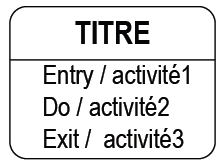
\includegraphics[width=1.10032in,height=0.82776in]{14-Logique/Cours/pandoc/media/image62.png}
\end{minipage} \\
\midrule\noalign{}
\endhead
\bottomrule\noalign{}
\endlastfoot
\textbf{\emph{do}} & Activités \textbf{interruptibles}. Elles sont \textbf{exécutées} dans l\textquotesingle{}\textbf{ordre} de leur \textbf{écriture}, à partir de l\textquotesingle instant où l'activité associée à \emph{entry} est terminée. & \\
\textbf{\emph{exit}} & Activité ayant une \textbf{fin}, elle ne peut \textbf{pas} être \textbf{interrompue}. Elle est \textbf{exécutée} lors de la \textbf{désactivation de l'état}, à l'instant de la sortie de l'état. & \\
\end{longtable}

\begin{quote}
Remarques~:

les trois comportements \textbf{\emph{entry}}, \textbf{\emph{do}} et \textbf{\emph{exit}} ne peuvent être \textbf{utilisés qu'une seule fois par état}, mais il est également possible de n'en \textbf{utiliser qu'une partie} (seulement \emph{entry} par exemple)~;

si \textbf{aucun mot} réservé n\textquotesingle est utilisé, cela correspond à un \emph{\textbf{do}~};

un \textbf{état vide} (sans activité) indique un \textbf{état d'attente}~;
\end{quote}

\begin{longtable}[]{@{}
  >{\raggedright\arraybackslash}p{(\columnwidth - 2\tabcolsep) * \real{0.1250}}
  >{\raggedright\arraybackslash}p{(\columnwidth - 2\tabcolsep) * \real{0.8611}}@{}}
\toprule\noalign{}
\begin{minipage}[b]{\linewidth}\raggedright
\begin{quote}
{[}{]} (14-Lo gique/ Cours/ pandoc /media /image 10.png )\{widt h=``0.6 262696 850393 701in''

height =``0.65 083333 333333 34in''\}
\end{quote}
\end{minipage} & \begin{minipage}[b]{\linewidth}\raggedright

\includegraphics[width=1.01042in,height=1.01042in]{14-Logique/Co urs/pandoc/media/image63.jpeg}\textbf{Lave-linge}

\textbf{Lister les états d'un graphe d'états qui permet de contrôler un lave-linge.}

Un cycle complet d'un lave-linge est composé de 5 états :

\begin{itemize}
\item
  Prélavage ;
\item
  Lavage ;
\item
  Rinçage ;
\item
  Essorage ;
\item
  Arrêt.
\end{itemize}

\begin{quote}
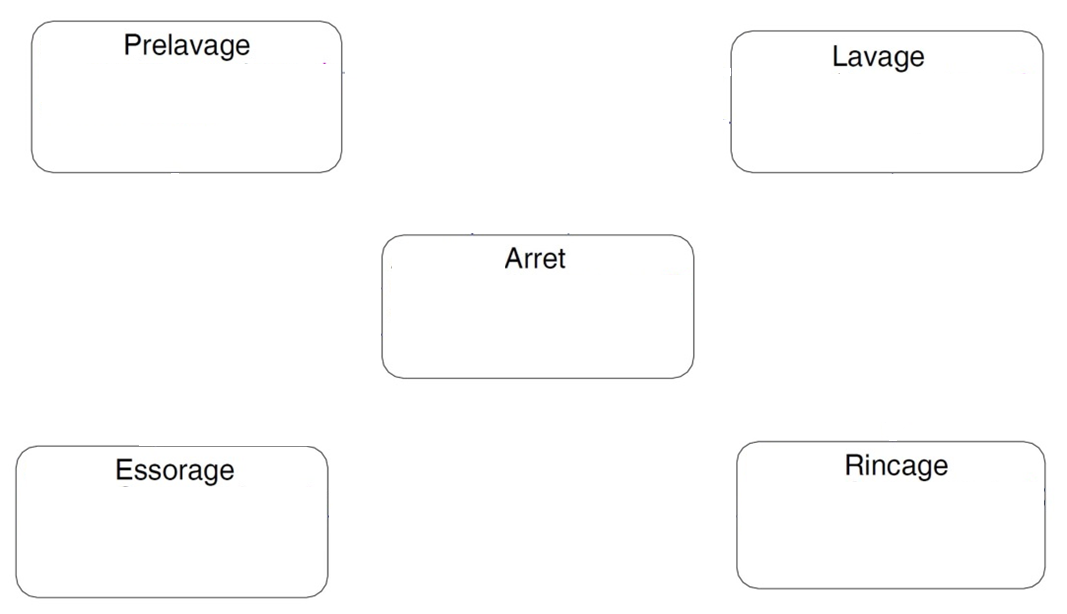
\includegraphics{14-Logique/Cours/pandoc/media/image64.png}
\end{quote}
\end{minipage} \\
\midrule\noalign{}
\endhead
\bottomrule\noalign{}
\endlastfoot
& \\
\end{longtable}

\begin{longtable}[]{@{}
  >{\raggedright\arraybackslash}p{(\columnwidth - 2\tabcolsep) * \real{0.1250}}
  >{\raggedright\arraybackslash}p{(\columnwidth - 2\tabcolsep) * \real{0.8611}}@{}}
\toprule\noalign{}
\begin{minipage}[b]{\linewidth}\raggedright
\begin{quote}
{[}{]} (14-Lo gique/ Cours/ pandoc /media /image 10.png )\{widt h=``0.6 262696 850393 701in''

height =``0.65 083333 333333 34in''\}
\end{quote}
\end{minipage} & \begin{minipage}[b]{\linewidth}\raggedright

\includegraphics[width=0.48958in,height=1.25698in]{14-Logique/Co urs/pandoc/media/image65.jpeg}\textbf{Feu Rouge}

\textbf{Lister les états d'un graphe d'états qui permet de contrôler un feu rouge.}
\end{minipage} \\
\midrule\noalign{}
\endhead
\bottomrule\noalign{}
\endlastfoot
& \\
\end{longtable}

\hypertarget{franchissement-des-transitions}{%
\subsubsection{Franchissement des transitions}\label{franchissement-des-transitions}}

Une fois recensés tous les états d'un système, il faut ensuite en modéliser ses évolutions en identifiant les conditions de changement d'état.

\begin{quote}
Une \textbf{transition} (représentée graphiquement par une flèche) modélise la possibilité d\textquotesingle un \textbf{passage} instantané d\textquotesingle un \textbf{état} vers \textbf{un autre}.

On appelle \textbf{état source} l\textquotesingle état de départ d\textquotesingle une transition, et \textbf{état cible} l\textquotesingle état d\textquotesingle arrivée d'une transition
\end{quote}

La \textbf{transition}~:

\begin{itemize}
\item
  est \textbf{instantanée} ;
\item
  n\textquotesingle est évaluée que si l\textquotesingle état source est actif.
\item
  Son \textbf{franchissement} est \textbf{conditionné} par des \textbf{événements déclencheurs} et des \textbf{conditions de garde}.
\end{itemize}

Ces événements et conditions de franchissement ainsi que l'éventuel effet associé à la transition sont indiqués le long de la flèche qui la symbolise suivant la notation~:

\begin{longtable}[]{@{}
  >{\raggedright\arraybackslash}p{(\columnwidth - 4\tabcolsep) * \real{0.4722}}
  >{\raggedright\arraybackslash}p{(\columnwidth - 4\tabcolsep) * \real{0.4583}}
  >{\raggedright\arraybackslash}p{(\columnwidth - 4\tabcolsep) * \real{0.0556}}@{}}
\toprule\noalign{}
\begin{minipage}[b]{\linewidth}\raggedright
\begin{quote}
\textbf{événement {[}garde{]} / effet}
\end{quote}
\end{minipage} & \begin{minipage}[b]{\linewidth}\raggedright
\end{minipage} & \begin{minipage}[b]{\linewidth}\raggedright
\end{minipage} \\
\midrule\noalign{}
\endhead
\bottomrule\noalign{}
\endlastfoot

\includegraphics[width=1.86607in,height=0.77975in]{14-Logiq ue/Cours/pandoc/media/image66.p ng} & Une transition réflexive entraîne une sortie de l\textquotesingle état puis un retour dans ce même état, avec appel des éventuelles activités \emph{exit} et \emph{entry}. & \\
\end{longtable}

\hypertarget{evuxe8nement}{%
\subsubsection{Evènement}\label{evuxe8nement}}

\begin{quote}
Un \textbf{événement} correspond au changement d'état d'une variable observée. Il est \textbf{daté} dans le temps et il est \textbf{traité instantanément} lors de son \textbf{occurrence} (front montant ou descendant) (apparition).
\end{quote}

\begin{longtable}[]{@{}
  >{\raggedright\arraybackslash}p{(\columnwidth - 2\tabcolsep) * \real{0.6250}}
  >{\raggedright\arraybackslash}p{(\columnwidth - 2\tabcolsep) * \real{0.3611}}@{}}
\toprule\noalign{}
\begin{minipage}[b]{\linewidth}\raggedright
Exemples~:

Appui sur un bouton, arrivée en fin de course d'un mécanisme, dépassement d'une valeur seuil\ldots{}
\end{minipage} & \begin{minipage}[b]{\linewidth}\raggedright
\end{minipage} \\
\midrule\noalign{}
\endhead
\bottomrule\noalign{}
\endlastfoot
& \\
\end{longtable}

\begin{quote}
Un \textbf{événement} n'est \textbf{jamais mémorisé} et est donc perdu s'il ne mène à aucune évolution du diagramme d'état.
\end{quote}

Il est possible d'utiliser des variables internes (compteurs ou horloge) pour spécifier un événement déclencheur~:

\begin{longtable}[]{@{}
  >{\raggedright\arraybackslash}p{(\columnwidth - 2\tabcolsep) * \real{0.1351}}
  >{\raggedright\arraybackslash}p{(\columnwidth - 2\tabcolsep) * \real{0.8378}}@{}}
\toprule\noalign{}
\begin{minipage}[b]{\linewidth}\raggedright
\emph{when}
\end{minipage} & \begin{minipage}[b]{\linewidth}\raggedright
Se déclenche lors du changement d'état d'une valeur interne au diagramme d'état. Il permet par exemple d'utiliser un compteur : \emph{when(N=3)}.
\end{minipage} \\
\midrule\noalign{}
\endhead
\bottomrule\noalign{}
\endlastfoot
\emph{after (T)} & se déclenche après une durée T passé dans l'état d'amont. Il permet de réaliser une temporisation. \\
\emph{at (D)} & se déclenche à la date D dans un référentiel de temps dont l'origine correspond généralement au démarrage du fonctionnement du système. \\
\end{longtable}

\begin{quote}
Si une \textbf{transition} n'a \textbf{pas d'événement} spécifié, l'\textbf{événement} déclencheur \textbf{implicite} est la fin des \textbf{d'activités} liées au \emph{\textbf{do} de l'\textbf{état source}}.
\end{quote}

\hypertarget{garde}{%
\subsubsection{Garde}\label{garde}}

\begin{quote}
La \textbf{garde} est une \textbf{condition de franchissement} de la transition. C'est une condition logique évaluée à l'instant de l'évènement déclencheur.
\end{quote}

Contrairement à l'événement qui, lui, est localisé dans le temps, la garde traduit une condition qui dure dans le temps et qui doit persister.

\begin{figure}
\centering
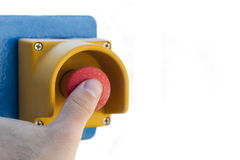
\includegraphics[width=0.91133in,height=1.01739in]{14-Logique/Cours/pandoc/media/image67.jpeg}
\caption{Résultat de recherche d\textquotesingle images pour "bouton arret urgence"}
\end{figure}

\begin{longtable}[]{@{}
  >{\raggedright\arraybackslash}p{(\columnwidth - 2\tabcolsep) * \real{0.6250}}
  >{\raggedright\arraybackslash}p{(\columnwidth - 2\tabcolsep) * \real{0.3611}}@{}}
\toprule\noalign{}
\begin{minipage}[b]{\linewidth}\raggedright
\textbf{Exemple}~:

Pour un bouton~:

- l'événement est associé à l'instant où le bouton est enfoncé~;

- la garde est associé à l'état du bouton~: enfoncé ou non.
\end{minipage} & \begin{minipage}[b]{\linewidth}\raggedright
\end{minipage} \\
\midrule\noalign{}
\endhead
\bottomrule\noalign{}
\endlastfoot
& \\
\end{longtable}

\begin{quote}
Si une \textbf{garde} n'est \textbf{pas présente} le long d'une transition, elle est \textbf{considérée} comme toujours \textbf{vraie}.
\end{quote}

La syntaxe d'une condition de garde vérifiant si l'état TOTO est actif est : {[}in TOTO{]}.

\hypertarget{equation-logique}{%
\subsubsection{Equation logique}\label{equation-logique}}

\begin{longtable}[]{@{}l@{}}
\toprule\noalign{}
\endhead
\bottomrule\noalign{}
\endlastfoot
La condition 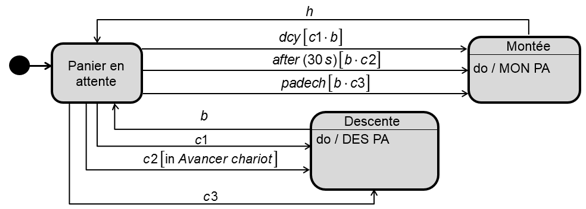
\includegraphics{14-Logique/Cours/pandoc/media/image68.png}\{width=``4.289864391951006in'' \\
\textbf{logique} évaluée height=``1.5300043744531933in''\} \\
pour la garde peut-être \\
le résultat d'une \\
combinaison de l'état \\
de plusieurs grandeurs \\
logiques, on parle \\
alors du résultat d'une \\
équation logique. \\
\end{longtable}

\begin{center}\rule{0.5\linewidth}{0.5pt}\end{center}

Dans ce type d'équation, on utilise des opérateurs logiques selon les règles de l'algèbre de BOOLE.

Ces 4 opérateurs logiques sont~: \textbf{OUI}, \textbf{NON}, \textbf{OU}, \textbf{ET}. Ils permettent de réaliser les opérations de base :

\begin{longtable}[]{@{}
  >{\raggedright\arraybackslash}p{(\columnwidth - 6\tabcolsep) * \real{0.3472}}
  >{\raggedright\arraybackslash}p{(\columnwidth - 6\tabcolsep) * \real{0.2083}}
  >{\raggedright\arraybackslash}p{(\columnwidth - 6\tabcolsep) * \real{0.2361}}
  >{\raggedright\arraybackslash}p{(\columnwidth - 6\tabcolsep) * \real{0.1806}}@{}}
\toprule\noalign{}
\begin{minipage}[b]{\linewidth}\raggedright
Entrées~: \textbf{a} et \textbf{b} résultat~: \textbf{S}
\end{minipage} & \begin{minipage}[b]{\linewidth}\raggedright
\end{minipage} & \begin{minipage}[b]{\linewidth}\raggedright
\end{minipage} & \begin{minipage}[b]{\linewidth}\raggedright
\end{minipage} \\
\midrule\noalign{}
\endhead
\bottomrule\noalign{}
\endlastfoot
\textbf{OUI} & notée \includegraphics{14-Log ique/Cours/p andoc/media/ image69.wmf} & \emph{qui donne à S la valeur 1 si et seulement si} & \includegraphics{14 -Logique/C ours/pando c/media/im age70.wmf} \\
\textbf{NON}

(appelé aussi «~complément~») & notée \includegraphics{14-Log ique/Cours/p andoc/media/ image71.wmf} & & \includegraphics{14 -Logique/C ours/pando c/media/im age72.wmf} \\
\textbf{OU}

(appelé aussi «~somme logique~») & notée \includegraphics{14-Log ique/Cours/p andoc/media/ image73.wmf} & & \includegraphics{14-L ogique/Cou rs/pandoc/ media/imag e74.wmf}OU \includegraphics{14 -Logique/C ours/pando c/media/im age75.wmf} \\
\textbf{ET}

(appelé aussi «~produit logique~») & notée \includegraphics{14-Log ique/Cours/p andoc/media/ image76.wmf} & & \includegraphics{14-L ogique/Cou rs/pandoc/ media/imag e77.wmf}ET \includegraphics{14 -Logique/C ours/pando c/media/im age78.wmf} \\
\end{longtable}

\begin{quote}
L'opérateur logique \textbf{OU} correspond à un montage en \textbf{parallèle}.

L'opérateur logique \textbf{ET} correspond à un montage en \textbf{série}.
\end{quote}

\hypertarget{effet}{%
\subsubsection{Effet}\label{effet}}

\begin{quote}
Un \textbf{effet} est une \textbf{activité} accomplie lorsque la \textbf{transition} est \textbf{franchie}.
\end{quote}

Les activités associées aux effets sont considérées instantanées, par exemple on peut définir une variable /N=1

\begin{quote}
Une transition peut ne pas avoir d'effet associé.
\end{quote}

\begin{longtable}[]{@{}
  >{\raggedright\arraybackslash}p{(\columnwidth - 2\tabcolsep) * \real{0.1250}}
  >{\raggedright\arraybackslash}p{(\columnwidth - 2\tabcolsep) * \real{0.8611}}@{}}
\toprule\noalign{}
\begin{minipage}[b]{\linewidth}\raggedright
\begin{quote}
{[}{]} (14-Lo gique/ Cours/ pandoc /media /image 10.png )\{widt h=``0.6 262696 850393 701in''

height =``0.65 083333 333333 34in''\}
\end{quote}
\end{minipage} & \begin{minipage}[b]{\linewidth}\raggedright

\includegraphics[width=0.48958in,height=1.25698in]{14-Logique/Co urs/pandoc/media/image65.jpeg}\textbf{Feu Rouge}

\textbf{Réaliser le graphe d'états du feu rouge.}
\end{minipage} \\
\midrule\noalign{}
\endhead
\bottomrule\noalign{}
\endlastfoot
& \\
\end{longtable}

\hypertarget{section}{%
\subsubsection*{}\label{section}}
\addcontentsline{toc}{subsubsection}{}

\hypertarget{pseudos-uxe9tats}{%
\subsubsection{Pseudos-états}\label{pseudos-uxe9tats}}

\begin{quote}
Un \textbf{pseudo-état} est un état ne pouvant \textbf{pas} avoir d'\textbf{activité}.
\end{quote}

Ils servent essentiellement comme éléments de liaison et pour indiquer l'état initial ou l'arrêt du diagramme d'état.

\hypertarget{pseudo-uxe9tat-initial}{%
\subparagraph*{\texorpdfstring{Pseudo-état initial \protect
\includegraphics[width=0.38511in,height=0.12134in]{14-Logique/Cours/pandoc/media/image79.png}}{Pseudo-état initial }}\label{pseudo-uxe9tat-initial}}
\addcontentsline{toc}{subparagraph}{Pseudo-état initial }

\begin{quote}
\textbf{Unique} et \textbf{obligatoire}, il est activé au \textbf{lancement} de la machine à états et marque le début de l'exécution du diagramme d'état. Il n'a aucune transition entrante.
\end{quote}

\hypertarget{pseudo-uxe9tat-final}{%
\subparagraph*{\texorpdfstring{Pseudo-état final \protect
\includegraphics[width=0.29581in,height=0.15777in]{14-Logique/Cours/pandoc/media/image80.png}}{Pseudo-état final }}\label{pseudo-uxe9tat-final}}
\addcontentsline{toc}{subparagraph}{Pseudo-état final }

\begin{quote}
\textbf{Optionnel}, il signe la \textbf{fin de l'exécution du diagramme d'état}. Il n'a aucune transition sortante.
\end{quote}

\hypertarget{pseudo-uxe9tat-jonction}{%
\subparagraph*{\texorpdfstring{Pseudo-état jonction \protect
\includegraphics[width=0.13822in,height=0.13822in]{14-Logique/Cours/pandoc/media/image81.png}}{Pseudo-état jonction }}\label{pseudo-uxe9tat-jonction}}
\addcontentsline{toc}{subparagraph}{Pseudo-état jonction }

\begin{quote}
Utilisé pour \textbf{regrouper} («~factoriser~») des \textbf{conditions de franchissement de transition}, en particulier des gardes communes à un événement.
\end{quote}

Il permet de partager des segments de transition et d'aboutir à une notation plus lisible des chemins alternatifs.

\begin{quote}
L'\textbf{évaluation} des \textbf{conditions de garde} en \textbf{aval} du pseudo-état est réalisée \textbf{avant} qu'il ne soit atteint.
\end{quote}

\begin{longtable}[]{@{}
  >{\raggedright\arraybackslash}p{(\columnwidth - 2\tabcolsep) * \real{0.1250}}
  >{\raggedright\arraybackslash}p{(\columnwidth - 2\tabcolsep) * \real{0.8611}}@{}}
\toprule\noalign{}
\begin{minipage}[b]{\linewidth}\raggedright
\begin{quote}
{[}{]} (14-Lo gique/ Cours/ pandoc /media /image 10.png )\{widt h=``0.6 262696 850393 701in''

height =``0.65 083333 333333 34in''\}
\end{quote}
\end{minipage} & \begin{minipage}[b]{\linewidth}\raggedright
\textbf{Pseudo état jonction}

\begin{longtable}[]{@{}
  >{\raggedright\arraybackslash}p{(\columnwidth - 2\tabcolsep) * \real{0.3889}}
  >{\raggedright\arraybackslash}p{(\columnwidth - 2\tabcolsep) * \real{0.3889}}@{}}
\toprule\noalign{}
\begin{minipage}[b]{\linewidth}\raggedright
\includegraphics{14-Logi que/Cours/pandoc/media/im age82.png}\{width=``2.77in'' heigh t=``1.3779472878390202in''\}

Exemple sans pseudo-état jonction
\end{minipage} & \begin{minipage}[b]{\linewidth}\raggedright

\includegraphics{14-Logique/Cours/pan doc/media/image83.png}\{wi dth=``2.717169728783902in'' heigh t=``1.3243055555555556in''\}

Exemple avec pseudo-état jonction
\end{minipage} \\
\midrule\noalign{}
\endhead
\bottomrule\noalign{}
\endlastfoot
& \\
\end{longtable}
\end{minipage} \\
\midrule\noalign{}
\endhead
\bottomrule\noalign{}
\endlastfoot
& \\
\end{longtable}

\hypertarget{pseudo-uxe9tat-duxe9cision}{%
\subparagraph*{\texorpdfstring{Pseudo-état décision \protect
\includegraphics[width=0.30771in,height=0.15178in]{14-Logique/Cours/pandoc/media/image84.png}}{Pseudo-état décision }}\label{pseudo-uxe9tat-duxe9cision}}
\addcontentsline{toc}{subparagraph}{Pseudo-état décision }

\begin{quote}
Utilisé pour une sélection ou une convergence de séquences exclusives.

L'\textbf{évaluation} des \textbf{conditions de garde} en \textbf{aval} du pseudo-état est réalisée \textbf{au moment} (contrairement au pseud état jonction) où il est atteint.

Les \textbf{conditions de gardes} doivent être \textbf{exclusives}.
\end{quote}

L\textquotesingle utilisation d\textquotesingle une clause {[}\emph{else}{]} est recommandée après un pseudo-état décision, car elle garantit un modèle correct en englobant tout ce qui n'est pas décrit dans les autres expressions logiques et en assurant ainsi qu'un moins un segment en aval est franchissable.

\begin{longtable}[]{@{}
  >{\raggedright\arraybackslash}p{(\columnwidth - 2\tabcolsep) * \real{0.1250}}
  >{\raggedright\arraybackslash}p{(\columnwidth - 2\tabcolsep) * \real{0.8611}}@{}}
\toprule\noalign{}
\begin{minipage}[b]{\linewidth}\raggedright
\begin{quote}
{[}{]} (14-Lo gique/ Cours/ pandoc /media /image 10.png )\{widt h=``0.6 262696 850393 701in''

height =``0.65 083333 333333 34in''\}
\end{quote}
\end{minipage} & \begin{minipage}[b]{\linewidth}\raggedright

\includegraphics[width=2.06597in,height=1.16597in]{14-Logique/C ours/pandoc/media/image85.emf}\textbf{Pseudo état jonction}

Ci-contre, dès que l'événement apparaît, le pseudo-état décision est atteint. Si la condition est vraie, c'est l'état 2 qui devient actif, sinon, c'est l'état 3.
\end{minipage} \\
\midrule\noalign{}
\endhead
\bottomrule\noalign{}
\endlastfoot
& \\
\end{longtable}

\begin{longtable}[]{@{}
  >{\raggedright\arraybackslash}p{(\columnwidth - 2\tabcolsep) * \real{0.1250}}
  >{\raggedright\arraybackslash}p{(\columnwidth - 2\tabcolsep) * \real{0.8611}}@{}}
\toprule\noalign{}
\begin{minipage}[b]{\linewidth}\raggedright
\begin{quote}
{[}{]} (14-Lo gique/ Cours/ pandoc /media /image 10.png )\{widt h=``0.6 262696 850393 701in''

height =``0.65 083333 333333 34in''\}
\end{quote}
\end{minipage} & \begin{minipage}[b]{\linewidth}\raggedright
\textbf{Vrai ou Faux}

\textbf{Ces deux portions de diagramme d'état décrivent-ils des comportements identiques~?}

! \href{14-Logique/Cours/pandoc/media/image86.png}{}

{[}{]} (14-Logique/Cours/pandoc/media/image87.png)\{width=``2.425in'' height=``1.2166666666666666in''\}

\textbf{Ce diagramme d'état est-il correct~?}

\textbf{Ces deux diagrammes d'état sont-ils équivalents~? Les gardes sont bien exclusives.}

{[}{]} (14-Logique/Cours/pandoc/media/image88.png)\{width=``5.575in'' height=``1.0416666666666667in''\}
\end{minipage} \\
\midrule\noalign{}
\endhead
\bottomrule\noalign{}
\endlastfoot
& \\
\end{longtable}

\hypertarget{uxe9tat-composite}{%
\subsubsection{État composite}\label{uxe9tat-composite}}

\begin{quote}
Un \textbf{état composite} décrit les \textbf{évolutions internes} d'un \textbf{état} à l'aide d'un \textbf{autre diagramme d'état}.

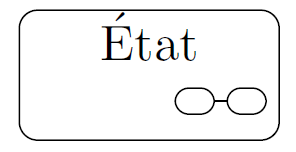
\includegraphics[width=0.87786in,height=0.45079in]{14-Logique/Cours/pandoc/media/image89.png}

Pour repérer un état composite, un signe symbolisant des lunettes est apposé sur l'état.
\end{quote}

Cette structure qui englobe plusieurs sous-états exclusifs considérés comme \emph{hiérarchiquement inférieur} au diagramme principal, permet de rendre ce dernier plus lisible en entrant séparément dans le détail des évolutions internes du système.

\begin{longtable}[]{@{}
  >{\raggedright\arraybackslash}p{(\columnwidth - 2\tabcolsep) * \real{0.1250}}
  >{\raggedright\arraybackslash}p{(\columnwidth - 2\tabcolsep) * \real{0.8611}}@{}}
\toprule\noalign{}
\begin{minipage}[b]{\linewidth}\raggedright
\begin{quote}
{[}{]} (14-Lo gique/ Cours/ pandoc /media /image 10.png )\{widt h=``0.6 262696 850393 701in''

height =``0.65 083333 333333 34in''\}
\end{quote}
\end{minipage} & \begin{minipage}[b]{\linewidth}\raggedright

\includegraphics[width=1.13542in,height=1.01667in]{14-Logique/C ours/pandoc/media/image90.png}\textbf{Radio-réveil}


\includegraphics[width=3.33882in,height=2.61561in]{14-Logique/C ours/pandoc/media/image91.png}
\includegraphics[width=3.50833in,height=1.46667in]{14-Logique/C ours/pandoc/media/image92.png}
\end{minipage} \\
\midrule\noalign{}
\endhead
\bottomrule\noalign{}
\endlastfoot
& \\
\end{longtable}

\begin{center}\rule{0.5\linewidth}{0.5pt}\end{center}

\begin{center}\rule{0.5\linewidth}{0.5pt}\end{center}

\begin{quote}
Une transition qui atteint la bordure d'un état composite est équivalente à une transition qui atteint l'état initial de sa région interne.

Une transition qui sort de la bordure d'un état composite est équivalente à une transition qui sort de tous les états de sa région interne.
\end{quote}

\hypertarget{historique-dun-uxe9tat-composite}{%
\subsubsection{Historique d'un état composite}\label{historique-dun-uxe9tat-composite}}

\begin{longtable}[]{@{}
  >{\raggedright\arraybackslash}p{(\columnwidth - 0\tabcolsep) * \real{1.0000}}@{}}
\toprule\noalign{}
\begin{minipage}[b]{\linewidth}\raggedright
\begin{quote}
L'\textbf{état actif} au \textbf{moment} de la \textbf{sortie} d'un \textbf{état composite} peut être \textbf{mémorisé} par l'indication \textbf{historique}.


\includegraphics[width=0.33542in,height=0.30417in]{14- Logique/Cours/pandoc/media/image93.png}

Lors de la \textbf{réactivation} de l'\textbf{état composite}, celui-ci se \textbf{réactive à cet état.}
\end{quote}
\end{minipage} \\
\midrule\noalign{}
\endhead
\bottomrule\noalign{}
\endlastfoot
 \\
\end{longtable}

\begin{longtable}[]{@{}
  >{\raggedright\arraybackslash}p{(\columnwidth - 2\tabcolsep) * \real{0.1250}}
  >{\raggedright\arraybackslash}p{(\columnwidth - 2\tabcolsep) * \real{0.8611}}@{}}
\toprule\noalign{}
\begin{minipage}[b]{\linewidth}\raggedright
\begin{quote}
{[}{]} (14-Lo gique/ Cours/ pandoc /media /image 10.png )\{widt h=``0.6 262696 850393 701in''

height =``0.65 083333 333333 34in''\}
\end{quote}
\end{minipage} & \begin{minipage}[b]{\linewidth}\raggedright
\textbf{Arrêt d'urgence}

L'\emph{historique} est utilisé ici pour permettre à un système de recommencer en cours de cycle lors du redémarrage après un appui sur l'arrêt d'urgence (ARU).

\begin{center}

\includegraphics[width=4.24432in,height=2.10668in]{14-Logique/ Cours/pandoc/media/image94.png}

C:\textbackslash Users\textbackslash ja ck\textbackslash AppData\textbackslash Local\textbackslash Temp\textbackslash SNAGHTML3652582b.PNG
\end{center}
\end{minipage} \\
\midrule\noalign{}
\endhead
\bottomrule\noalign{}
\endlastfoot
& \\
\end{longtable}

\hypertarget{uxe9tat-composite-orthogonal}{%
\subsubsection{État composite orthogonal~}\label{uxe9tat-composite-orthogonal}}

\begin{quote}
Dans un \textbf{état composite orthogonal}, \textbf{plusieurs diagrammes d\textquotesingle états} peuvent évoluer \textbf{simultanément} dans des \textbf{régions} séparées par des pointillés.

Les \textbf{différentes régions} de l'état orthogonal \textbf{fonctionnent} en \textbf{parallèle} sans \textbf{aucune influence} les unes sur les autres (plusieurs états sont actifs en même temps).

Une \textbf{transition} qui atteint la \textbf{bordure} d'un état \textbf{composite orthogonal} est \textbf{équivalente} à une \textbf{transition} qui atteint les \textbf{états initiaux} de \textbf{toutes} ses \textbf{régions}.

\textbf{Toutes} les \textbf{régions} d'un \textbf{état composite orthogonal} doivent \textbf{atteindre} leur \textbf{état final} pour que l'\textbf{état composite} soit considéré comme \textbf{terminé}. Ce n'est qu'à cette condition que la \textbf{transition} de \textbf{sortie} de l\textquotesingle{}\textbf{état composite} devient \textbf{franchissable}.
\end{quote}

\begin{longtable}[]{@{}
  >{\raggedright\arraybackslash}p{(\columnwidth - 2\tabcolsep) * \real{0.1250}}
  >{\raggedright\arraybackslash}p{(\columnwidth - 2\tabcolsep) * \real{0.8611}}@{}}
\toprule\noalign{}
\begin{minipage}[b]{\linewidth}\raggedright
\begin{quote}
{[}{]} (14-Lo gique/ Cours/ pandoc /media /image 10.png )\{widt h=``0.6 262696 850393 701in''

height =``0.65 083333 333333 34in''\}
\end{quote}
\end{minipage} & \begin{minipage}[b]{\linewidth}\raggedright

\includegraphics[width=0.45432in,height=1.02273in]{14-Logique/Co urs/pandoc/media/image95.jpeg}\textbf{Distributeur de boissons}


\includegraphics[width=5.62729in,height=1.76515in]{14-Logique/C ours/pandoc/media/image96.emf}
\end{minipage} \\
\midrule\noalign{}
\endhead
\bottomrule\noalign{}
\endlastfoot
& \\
\end{longtable}

\begin{quote}
L'\textbf{activation} et la \textbf{sortie} d'un \textbf{état composite} \textbf{orthogonal} peuvent être également symbolisés par des \textbf{barres de synchronisation \emph{fork}} et \textbf{\emph{join}} qui fonctionnent par paire.

Les \textbf{transitions,} nécessairement \textbf{automatiques}, qui \textbf{partent} d\textquotesingle une barre de synchronisation \textbf{\emph{fork}} sont \textbf{franchies simultanément}.

La \textbf{transition} qui \textbf{part} d'une barre de synchronisation \textbf{\emph{join}} n'est \textbf{franchissable} qu\textquotesingle après le \textbf{franchissement} de \textbf{toutes} les \textbf{transitions,} nécessairement \textbf{automatiques}, qui \textbf{convergent} vers cette barre.
\end{quote}

\begin{longtable}[]{@{}
  >{\raggedright\arraybackslash}p{(\columnwidth - 2\tabcolsep) * \real{0.1250}}
  >{\raggedright\arraybackslash}p{(\columnwidth - 2\tabcolsep) * \real{0.8611}}@{}}
\toprule\noalign{}
\begin{minipage}[b]{\linewidth}\raggedright
\begin{quote}
{[}{]} (14-Lo gique/ Cours/ pandoc /media /image 10.png )\{widt h=``0.6 262696 850393 701in''

height =``0.65 083333 333333 34in''\}
\end{quote}
\end{minipage} & \begin{minipage}[b]{\linewidth}\raggedright

\includegraphics[width=0.45432in,height=1.02273in]{14-Logique/Co urs/pandoc/media/image95.jpeg}\textbf{Distributeur de boissons}


\includegraphics[width=5.69033in,height=1.89394in]{14-Logique/ Cours/pandoc/media/image97.emf}
\end{minipage} \\
\midrule\noalign{}
\endhead
\bottomrule\noalign{}
\endlastfoot
& \\
\end{longtable}

\begin{longtable}[]{@{}
  >{\raggedright\arraybackslash}p{(\columnwidth - 2\tabcolsep) * \real{0.1250}}
  >{\raggedright\arraybackslash}p{(\columnwidth - 2\tabcolsep) * \real{0.8611}}@{}}
\toprule\noalign{}
\begin{minipage}[b]{\linewidth}\raggedright
\begin{quote}
{[}{]} (14-Lo gique/ Cours/ pandoc /media /image 10.png )\{widt h=``0.6 262696 850393 701in''

height =``0.65 083333 333333 34in''\}
\end{quote}
\end{minipage} & \begin{minipage}[b]{\linewidth}\raggedright
\textbf{Turbine à gaz}

La plupart des pays de l'Union Européenne ont entamé une transition énergétique afin de réduire les émissions des gaz à effet de serre. Ainsi, la part des énergies renouvelables comme le solaire ou l'éolien augmente. Leur principal inconvénient est leur intermittence. Il est alors nécessaire de disposer de sources permettant de pallier ce défaut. Les turbines à gaz (\textbf{figure 1}) sont souvent la solution privilégiée pour leur rendement, leur réactivité et leur impact environnemental. Ce sont des machines tournantes thermodynamiques appartenant à la famille des moteurs à combustion interne. Elles peuvent produire de l'électricité et de la chaleur à partir de la combustion du gaz.

Du fait de leur taille relativement réduite et de leur capacité de production, ces turbines sont aussi parfois installées loin de toute autre source d'énergie (plateformes maritimes par exemple) afin de fournir électricité et chaleur. Ces types de sources d'énergie sont aussi utilisés dans divers bâtiments (usines, universités, bâtiments publics en tout genre) comme source de secours en cas de panne de la source principale d'énergie.


\includegraphics[width=2.56875in,height=4.34028in]{1 4-Logique/Cours/pandoc/media/image98.png}
\includegraphics[width=4.388in,height=1.76013in]{14-Logique/C ours/pandoc/media/image99.png}


\includegraphics[width=2.88611in,height=1.66944in]{14-Logique/C ours/pandoc/media/image100.png}Le principe de fonctionnement de ces turbines (schématisé sur la \textbf{figure 2}) repose sur la combustion d'un gaz (G) injecté dans une chambre de combustion (Ch). Ce gaz mélangé à de l'air (E) comprimé via un compresseur à ailettes (C) est brûlé mettant ainsi en rotation un arbre (A) par l'intermédiaire de roues à aubes (T) par lesquelles passe le gaz de combustion. La rotation de cet arbre permet ensuite de générer un courant électrique par l'intermédiaire d'un alternateur (non représenté sur la \textbf{figure 2}). Les gaz d'échappement (Ec) peuvent ensuite être utilisés pour produire de la chaleur.

\textbf{Figure 2 -} Schéma de principe de fonctionnement d'une turbine gaz

Il est toutefois à noter que ce principe ne fonctionne qu'une fois la turbine déjà lancée. Il est donc nécessaire de disposer d'un système de lancement électrique ou pneumatique.

Le démarrage de la turbine est décrit par le diagramme d'état.

\textbf{À l'aide des éléments précédents, compléter le chronogramme.}


\includegraphics[width=5.7861in,height=2.78271in]{14-Logique/C ours/pandoc/media/image101.png}

Les variables associées à ce chronogramme sont notées ainsi :

- E représente l'état embrayé (le moteur de démarrage entraîne l'arbre de la turbine) ;

- D représente l'état débrayé (le moteur de démarrage n'entraîne plus l'arbre) ;

- AV représente la phase d'augmentation de vitesse du moteur grâce au variateur (état à 1

lorsque la vitesse augmente, 0 sinon) ;

- C représente l'état du capteur de vitesse (son état est à 1 lorsque la vitesse du moteur atteint la vitesse d'autonomie \emph{Ntr}, sinon son état est 0).


\includegraphics[width=0.98542in,height=1.50417in]{14-Logique/Co urs/pandoc/media/image102.emf}E\textbf{n déduire le temps de cycle de démarrage et le comparer au cahier des charges.}
\end{minipage} \\
\midrule\noalign{}
\endhead
\bottomrule\noalign{}
\endlastfoot
& \\
\end{longtable}

\hypertarget{diagramme-de-suxe9quence-sd}{%
\subsection{Diagramme de séquence~(sd)}\label{diagramme-de-suxe9quence-sd}}

Un autre diagramme du langage SysML permet de décrire le \textbf{comportement} séquentiel d'un système. Il s'agit du diagramme de séquence.

\hypertarget{diagramme-de-suxe9quence}{%
\subsubsection{Diagramme de séquence}\label{diagramme-de-suxe9quence}}

Un diagramme de séquence est rattaché à un cas d'utilisation et décrit ce dernier en entier ou en partie, ce qui correspond à un scénario de fonctionnement possible, défini dans un cadre précis.

\begin{quote}
Il décrit, dans l'\textbf{ordre chronologique}, l'\textbf{enchaînement} des \textbf{interactions} (ou messages) entre les \textbf{acteurs} du système ou entre des \textbf{composants} du système eux-mêmes.
\end{quote}

Les principaux éléments sont~:

\begin{longtable}[]{@{}
  >{\raggedright\arraybackslash}p{(\columnwidth - 14\tabcolsep) * \real{0.1220}}
  >{\raggedright\arraybackslash}p{(\columnwidth - 14\tabcolsep) * \real{0.0732}}
  >{\raggedright\arraybackslash}p{(\columnwidth - 14\tabcolsep) * \real{0.1463}}
  >{\raggedright\arraybackslash}p{(\columnwidth - 14\tabcolsep) * \real{0.1829}}
  >{\raggedright\arraybackslash}p{(\columnwidth - 14\tabcolsep) * \real{0.2439}}
  >{\raggedright\arraybackslash}p{(\columnwidth - 14\tabcolsep) * \real{0.0610}}
  >{\raggedright\arraybackslash}p{(\columnwidth - 14\tabcolsep) * \real{0.0488}}
  >{\raggedright\arraybackslash}p{(\columnwidth - 14\tabcolsep) * \real{0.0488}}@{}}
\toprule\noalign{}
\begin{minipage}[b]{\linewidth}\raggedright
\textbf{Ligne de vie}
\end{minipage} & \begin{minipage}[b]{\linewidth}\raggedright
Li gne ver tic ale en po int ill ée. Une p our cha que é lém ent d ial ogu ant (a cte ur, sy stè me, sou s-s yst ème ou co mpo san t).
\end{minipage} & \begin{minipage}[b]{\linewidth}\raggedright
\end{minipage} & \begin{minipage}[b]{\linewidth}\raggedright
\end{minipage} & \begin{minipage}[b]{\linewidth}\raggedright
\end{minipage} & \begin{minipage}[b]{\linewidth}\raggedright
\end{minipage} & \begin{minipage}[b]{\linewidth}\raggedright
\end{minipage} & \begin{minipage}[b]{\linewidth}\raggedright
\end{minipage} \\
\midrule\noalign{}
\endhead
\bottomrule\noalign{}
\endlastfoot
\textbf{ Période d'act ivité} & Ba nde ver tic ale sur une li gne de v ie. Opt ion nel les el les f aci lit ent la l ect ure du d iag ram me. & & & & & & \\
\textbf{Me ssage} & \begin{minipage}[t]{\linewidth}\raggedright
Flè che ho riz ont ale un idi rec tio nne lle en tre d eux lig nes de vie rep rés ent ant un é lém ent de co mmu nic ati on. E lle déc len che une p éri ode d 'ac tiv ité (un c omp ort eme nt) c hez le re cev eur du me ssa ge, p our q ui, l \textquotesingle a rri vée d\\
'un m ess age est un évé nem ent déc len che ur.

Ce m ess age p eut êtr e~:\strut
\end{minipage} & & & & & & \\
& \begin{minipage}[t]{\linewidth}\raggedright
\begin{itemize}
\item
  sy nch ron e~:

  l\\
  'ém ett eur
\end{itemize}

att end

une

ré pon se,

son

com por tem ent

est

blo qué

p end ant

l' att ent e~;\strut
\end{minipage} & & & & & & \\
& \begin{minipage}[t]{\linewidth}\raggedright
\begin{itemize}
\tightlist
\item
\end{itemize}

asy nch ron e~:

l\\
'ém ett eur

n\textquotesingle{} att end

pas

de

ré pon se,

son

com por tem ent

con tin u~;\strut
\end{minipage} & & & & & & \\
& \begin{minipage}[t]{\linewidth}\raggedright
\begin{itemize}
\tightlist
\item
\end{itemize}

une

ré pon se.
\end{minipage} & & & & & & \\
& \begin{minipage}[t]{\linewidth}\raggedright
Il est po ssi ble d\\
'av oir un m ess age ré fle xif c orr esp ond ant à une in ter act ion i nte rne au c omp osa nt.\strut
\end{minipage} & & & & & & \\
\textbf{Fra gment} & Ca dre eng lob ant une par tie de la sé que nce & & & & & & \\
& \begin{minipage}[t]{\linewidth}\raggedright
\begin{itemize}
\tightlist
\item
  \textbf{l oop }*
\end{itemize}
\end{minipage} & Boucle, le fragment est maintenu pendant une durée qui dépend de la condition de garde. & & \includegraphics{14- Logique/Cours/pan doc/media/image10 3.png} & & & \\
& \begin{minipage}[t]{\linewidth}\raggedright
\begin{center}\rule{0.5\linewidth}{0.5pt}\end{center}

par ***
\end{minipage} & Séquence en p arallèle. Les régions peuvent être exécutées simul tanément. & & \includegraphics{14-L ogique/Cours/pand oc/media/image104 .png} & & & \\
& \begin{minipage}[t]{\linewidth}\raggedright
\begin{center}\rule{0.5\linewidth}{0.5pt}\end{center}

alt ***
\end{minipage} & Séquences alt ernatives condi tionnées. Seule la région dont la condition est vraie s 'exécute. & & \includegraphics{14-L ogique/Cours/pand oc/media/image105 .png} & & & \\
& & & & & & & \\
\end{longtable}

\begin{longtable}[]{@{}
  >{\raggedright\arraybackslash}p{(\columnwidth - 2\tabcolsep) * \real{0.1250}}
  >{\raggedright\arraybackslash}p{(\columnwidth - 2\tabcolsep) * \real{0.8611}}@{}}
\toprule\noalign{}
\begin{minipage}[b]{\linewidth}\raggedright
\begin{quote}
{[}{]} (14-Lo gique/ Cours/ pandoc /media /image 10.png )\{widt h=``0.6 262696 850393 701in''

height =``0.65 083333 333333 34in''\}
\end{quote}
\end{minipage} & \begin{minipage}[b]{\linewidth}\raggedright

\includegraphics[width=1.07482in,height=1.06981in]{14-Logique/C ours/pandoc/media/image106.png}
\includegraphics[width=1.23674in,height=0.67614in]{14-Logique/C ours/pandoc/media/image107.png}\textbf{Système de vente de repas en ligne}


\includegraphics[width=5.4625in,height=4.55417in]{1 4-Logique/Cours/pandoc/media/image108.png}
\end{minipage} \\
\midrule\noalign{}
\endhead
\bottomrule\noalign{}
\endlastfoot
& \\
\end{longtable}

\hypertarget{codeur-incremental-et-absolu}{%
\subsection{CODEUR INCREMENTAL ET ABSOLU}\label{codeur-incremental-et-absolu}}

\hypertarget{familles-de-capteurs}{%
\subsubsection{Familles de capteurs}\label{familles-de-capteurs}}

Pour contrôler le bon fonctionnement d\textquotesingle une chaîne d\textquotesingle énergie, il est nécessaire de mesurer des grandeurs physiques. Les 3 types de capteurs qui permettent d\textquotesingle acquérir des grandeurs sont :

\begin{itemize}
\item
  \textbf{les capteurs :} délivre une information \textbf{analogique} \textgreater{} (potentiomètre linéaire, rotatif, règle magnétique, cellule \textgreater{} magnétorésistive, tachymètre , génératrice tachymétrique, \textgreater{} accéléromètre, débitmètre, dynamomètre, jauges de déformation, \textgreater{} cellules pièzo-électriques, manomètre...)
\item
  \textbf{les codeurs :} délivre une information \textbf{numérique} (codeur \textgreater{} incrémental, absolu)
\item
  \textbf{les détecteurs :} délivre une information \textbf{logique} (détecteur \textgreater{} fin de course ILS, détecteur à effet hall, boutons...)
\end{itemize}

\hypertarget{vocabulaire-de-muxe9trologie}{%
\subsubsection{Vocabulaire de métrologie}\label{vocabulaire-de-muxe9trologie}}

\begin{quote}
\textbf{Résolution :} Plus petite variation de grandeur mesurable par le capteur.

\emph{\ul{Ex :} Le codeur incrémental à une résolution de 0,087°.}

\textbf{Sensibilité :} Variation du signal de sortie par rapport à la variation du signal d\textquotesingle entrée. \emph{\ul{Ex :} Le capteur de température LM35 a une sensibilité de 10mV/°C.}
\end{quote}

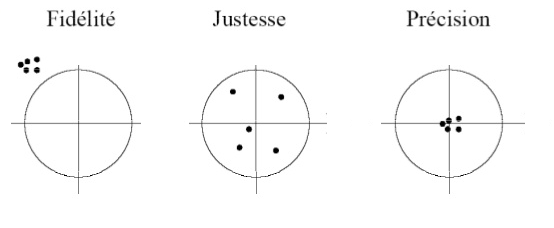
\includegraphics[width=2.26944in,height=0.93819in]{14-Logique/Cours/pandoc/media/image109.png}

\begin{quote}
\textbf{Fidélité :} Répétabilité de la mesure

\textbf{Justesse :} Réponse proche de la valeur vraie.

\textbf{Précision :} Écart entre la valeur vraie et la valeur mesurée.
\end{quote}

\hypertarget{les-codeurs}{%
\subsubsection{Les codeurs}\label{les-codeurs}}

\textbf{Le codeur est généralement placé en amont du réducteur}, car pour un même mouvement, on obtient plus d\textquotesingle impulsion et donc une meilleure résolution.

\hypertarget{codeur-incruxe9mental-ou-roue-codeuse}{%
\subparagraph*{Codeur incrémental (ou roue codeuse)}\label{codeur-incruxe9mental-ou-roue-codeuse}}
\addcontentsline{toc}{subparagraph}{Codeur incrémental (ou roue codeuse)}

\begin{quote}
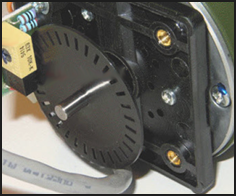
\includegraphics[width=1.57047in,height=1.33044in]{14-Logique/Cours/pandoc/media/image111.png}\ul{Codeur incrémental (ou roue codeuse) :}

Un codeur incrémental est un générateur d'\textbf{impulsions} qui fournit 2 voies en \textbf{quadrature} et un top zéro. Elles sont divisées en n secteurs angulaires égaux, alternativement opaques et transparents.

Ils fonctionnent sur le principe de \textbf{comptage} et \textbf{décomptage} \textbf{d\textquotesingle impulsions} et donne donc le déplacement relatif.

n s\textquotesingle appelle le nombre de périodes, c\textquotesingle est le nombre d\textquotesingle impulsions qui sont délivrées par le codeur pour un tour complet de son disque.

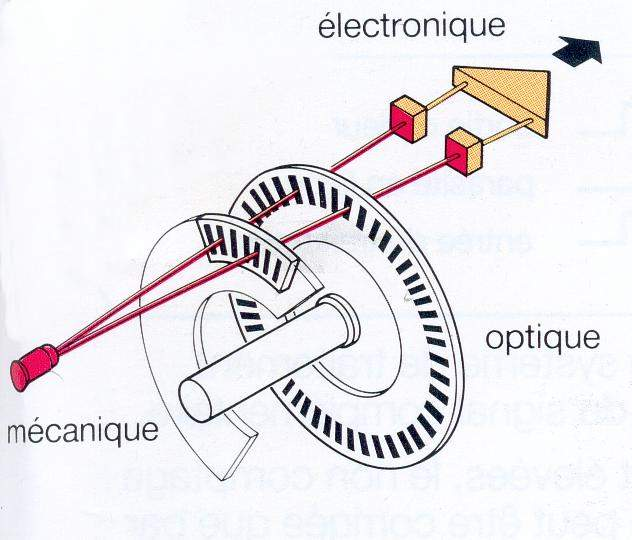
\includegraphics[width=2.10486in,height=1.80208in]{14-Logique/Cours/pandoc/media/image112.jpeg}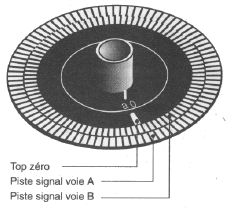
\includegraphics[width=2.37222in,height=2.1625in]{14-Logique/Cours/pandoc/media/image113.png}
\end{quote}

\textbf{Avantages :}

\begin{quote}
Mesure prise à coût raisonnable ;

Entrées de comptage adaptées (voies A, B, Z) en standard sur les automates programmables récents ;

Obtention aisée de la vitesse par intégration numérique.

\textbf{Inconvénients :}

Perte totale des informations en cas de coupure d\textquotesingle énergie ;

Nécessite une procédure de prise d\textquotesingle origine.
\end{quote}

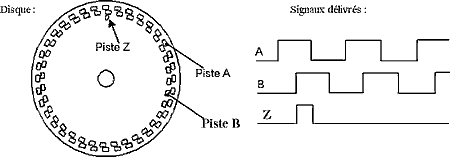
\includegraphics[width=1.61389in,height=0.96458in]{14-Logique/Cours/pandoc/media/image114.png}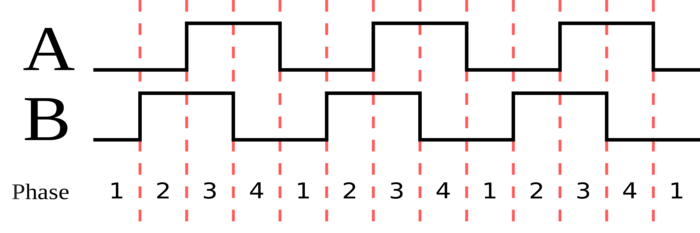
\includegraphics[width=2.67708in,height=0.88681in]{14-Logique/Cours/pandoc/media/image115.png}

Disque d\textquotesingle un codeur incrémental et pistes en quadrature de phase

\begin{quote}
Les pistes intérieures et extérieures sont en \textbf{quadrature de phase}, ce qui permet de :
\end{quote}

\begin{itemize}
\item
  connaitre le \textbf{sens de rotation} du capteur
\item
  \textbf{améliorer par 2 la résolution} du capteur.
\end{itemize}

\begin{longtable}[]{@{}
  >{\raggedright\arraybackslash}p{(\columnwidth - 2\tabcolsep) * \real{0.5139}}
  >{\raggedright\arraybackslash}p{(\columnwidth - 2\tabcolsep) * \real{0.4722}}@{}}
\toprule\noalign{}
\begin{minipage}[b]{\linewidth}\raggedright
\begin{quote}
Déterminer le sens de rotation
\end{quote}
\end{minipage} & \begin{minipage}[b]{\linewidth}\raggedright
\end{minipage} \\
\midrule\noalign{}
\endhead
\bottomrule\noalign{}
\endlastfoot
\begin{minipage}[t]{\linewidth}\raggedright
\begin{quote}
\includegraphics[width=2.18786in,height=1.16522in]{14 -Logique/Cours/pandoc/media/image1 18.png}

Le front montant de la voie verte se présente avant celui de la voie rouge.
\end{quote}
\end{minipage} & \begin{minipage}[t]{\linewidth}\raggedright
\begin{quote}

\includegraphics{14-Logiqu e/Cours/pandoc/media/image119.p ng}\{width=``2.178814523184602in''

height=``1.1652187226596675in''\}

Le front montant de la voie rouge se présente avant celui de la voie verte.
\end{quote}
\end{minipage} \\
\end{longtable}

\hypertarget{codeur-absolu-ou-numuxe9rique}{%
\subparagraph*{\texorpdfstring{\protect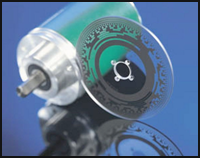
\includegraphics[width=1.26543in,height=1.02609in]{14-Logique/Cours/pandoc/media/image120.png}Codeur absolu (ou numérique)}{Codeur absolu (ou numérique)}}\label{codeur-absolu-ou-numuxe9rique}}
\addcontentsline{toc}{subparagraph}{Codeur absolu (ou numérique)}

\begin{quote}
\ul{Codeur absolu (ou numérique) :}

Délivre un signal image de la position à mesurer \textbf{sous forme d\textquotesingle un code numérique binaire} et donne le déplacement absolu.

Il dispose de N pistes, généralement agencées suivant le code \textbf{Gray}.

La piste intérieure correspond au bit de poids le plus fort.

\textbf{Avantages :}
\end{quote}

\begin{itemize}
\item
  Chaque secteur possédant son code unique, il est inutile de \textgreater{} déterminer le sens de rotation ;
\item
  Pas de perte d\textquotesingle information en cas de coupure d\textquotesingle énergie ;
\item
  Code connu en permanence, pas besoin de procéder à la Prise \textgreater{} d\textquotesingle Origine Machine lors de la mise sous tension ;
\item
  Pas d\textquotesingle erreur de lecture avec le code Gray.
\end{itemize}

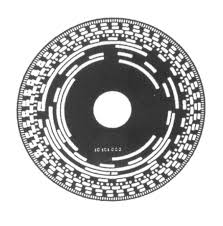
\includegraphics[width=1.06458in,height=1.03681in]{14-Logique/Cours/pandoc/media/image121.png}

\begin{quote}
\textbf{Inconvénients :}
\end{quote}

\begin{itemize}
\item
  Relativement onéreux ;
\item
  Interface avec la commande plus complexe (N entrées) ;
\item
  Nécessite un transcodeur pour reconvertir le signal en binaire \textgreater{} naturel.
\end{itemize}

\begin{longtable}[]{@{}
  >{\raggedright\arraybackslash}p{(\columnwidth - 2\tabcolsep) * \real{0.1250}}
  >{\raggedright\arraybackslash}p{(\columnwidth - 2\tabcolsep) * \real{0.8611}}@{}}
\toprule\noalign{}
\begin{minipage}[b]{\linewidth}\raggedright
\begin{quote}
{[}{]} (14-Lo gique/ Cours/ pandoc /media /image 10.png )\{widt h=``0.6 262696 850393 701in''

height =``0.65 083333 333333 34in''\}
\end{quote}
\end{minipage} & \begin{minipage}[b]{\linewidth}\raggedright
\textbf{Simulateur de moto - Codeur incrémental -- Asservissement d'un vérin}


\includegraphics[width=1.50069in,height=1.55in]{14-Logique/Co urs/pandoc/media/image122.emf}

Les usagers de deux-roues motorisés sont soumis à un risque accru d'accidents en comparaison aux autres catégories d'usagers.

Dans le but de réduire ce risque, la simulation de conduite offre une nouvelle opportunité pour appréhender le comportement des conducteurs dans un cadre sécuritaire et constitue un outil alternatif pour la formation à la conduite.


\includegraphics[width=5.89792in,height=2.55486in]{14-Logique/C ours/pandoc/media/image123.png}

Le capteur de position utilisé est un codeur optique composé de deux voies (Voies A et B) qui permettent de détecter le sens de rotation. Le diagramme d'état du document réponse DR4 décrit le comptage des impulsions Nmes. L'allure des signaux reçus (après traitement électronique) est donnée sur la figure 16.


\includegraphics[width=5.89792in,height=2.19306in]{14-Logique/C ours/pandoc/media/image124.png}


\includegraphics[width=5.89792in,height=1.52083in]{14-Logique/C ours/pandoc/media/image125.png}

\textbf{Compléter sur le document réponse, le chronogramme donnant l'évolution de la valeur N\textsubscript{mes} renvoyée par le compteur. Indiquer sur le diagramme d'état à quel numéro de mesure (mesures numérotées sur la figure 16) correspond chacun des états.}

Le complément de la variable logique A (respectivement B) est noté !A respectivement !B) sur le diagramme. Selon le contexte, la notation A pourra se référer à un évènement ou à une condition de garde.


\includegraphics[width=5.89792in,height=2.63194in]{14-Logique/C ours/pandoc/media/image126.png}


\includegraphics[width=5.89792in,height=4.38472in]{14-Logique/C ours/pandoc/media/image127.png}

\textbf{En vous appuyant sur le diagramme de définition de blocs (figure 13) et sur le schéma bloc de l'asservissement (figure 14), donner la valeur du gain K\textsubscript{cap} du codeur.}
\end{minipage} \\
\midrule\noalign{}
\endhead
\bottomrule\noalign{}
\endlastfoot
& \\
\end{longtable}

\hypertarget{reseaux-et-bus-de-terrain}{%
\subsection{RESEAUX ET BUS DE TERRAIN}\label{reseaux-et-bus-de-terrain}}

\hypertarget{introduction-sur-les-donnuxe9es}{%
\subsubsection{Introduction sur les données}\label{introduction-sur-les-donnuxe9es}}

Aujourd'hui, de nombreux types de données doivent être transmises~:

\begin{itemize}
\item
  La parole et son haute-fidélité;
\item
  Des données alphanumériques (texte, fichiers de données,\ldots);
\item
  Des images fixes (N/B et couleurs);
\item
  Images animées (Télévision par exemple);
\item
  Informations multimédias (Combinaisons précédentes)
\end{itemize}

La transmission de données aura alors plusieurs critères de performances (disponibilité, taux d'erreur, débit, \ldots.)

\hypertarget{qualituxe9-de-service-qos}{%
\subsubsection{Qualité de service~: QoS}\label{qualituxe9-de-service-qos}}

Elle se traduit sous différentes exigences :

\begin{itemize}
\item
  La disponibilité des moyens de transfert de l'information (liés au taux de panne des équipements et liaisons);
\item
  Le taux d'erreur maximal, exprimé par le rapport entre le nombre de bits dont la valeur est modifiée par rapport au nombre total de bits d'informations émis ;
\item
  Le débit de transfert ;
\item
  Le délai, c'est à dire, la durée entre la décision d'émettre et la réception par le destinataire.
\end{itemize}

Ces exigences varient en fonction de la nature des informations à transmettre.

\begin{longtable}[]{@{}
  >{\raggedright\arraybackslash}p{(\columnwidth - 8\tabcolsep) * \real{0.1728}}
  >{\raggedright\arraybackslash}p{(\columnwidth - 8\tabcolsep) * \real{0.2222}}
  >{\raggedright\arraybackslash}p{(\columnwidth - 8\tabcolsep) * \real{0.2099}}
  >{\raggedright\arraybackslash}p{(\columnwidth - 8\tabcolsep) * \real{0.1852}}
  >{\raggedright\arraybackslash}p{(\columnwidth - 8\tabcolsep) * \real{0.1852}}@{}}
\toprule\noalign{}
\endhead
\bottomrule\noalign{}
\endlastfoot
& \textbf{Importance de la disponibilité} & \textbf{Importance du Taux d'erreur} & \textbf{Importance du Débit} & \textbf{Importance du Délai} \\
\textbf{Voix} & Important & Peu important & Peu important & Très faible ou constant \\
\textbf{Images animées} & Peu important & Peu important & Très important & Très faible \\
\textbf{Texte, images fixes} & Important & Très faible (10\textsuperscript{-9}) & Peu important & Peu important \\
\end{longtable}

\hypertarget{architecture-des-ruxe9seaux-de-communication}{%
\subsubsection{Architecture des réseaux de communication}\label{architecture-des-ruxe9seaux-de-communication}}

Dans l'architecture d'un réseau, on peut distinguer quatre catégories de réseaux (en fonction de l'étendue de leur zone de fonctionnement) :

\begin{itemize}
\item
  le réseau personnel : PAN (Personal Area Network) qui relie des machines sur quelques mètres~;
\item
  le réseau local : LAN (Local Area Network) qui est adapté à la taille d'un site d'entreprise;
\item
  le réseau métropolitain : MAN (Metropolitan Area Network) qui est un réseau étendu à l'échelle d'une ville ;
\item
  le réseau étendu : WAN (Wide Area Network) qui couvre une grande zone géographique (typiquement à l'échelle d'un pays, d'un continent).
\end{itemize}

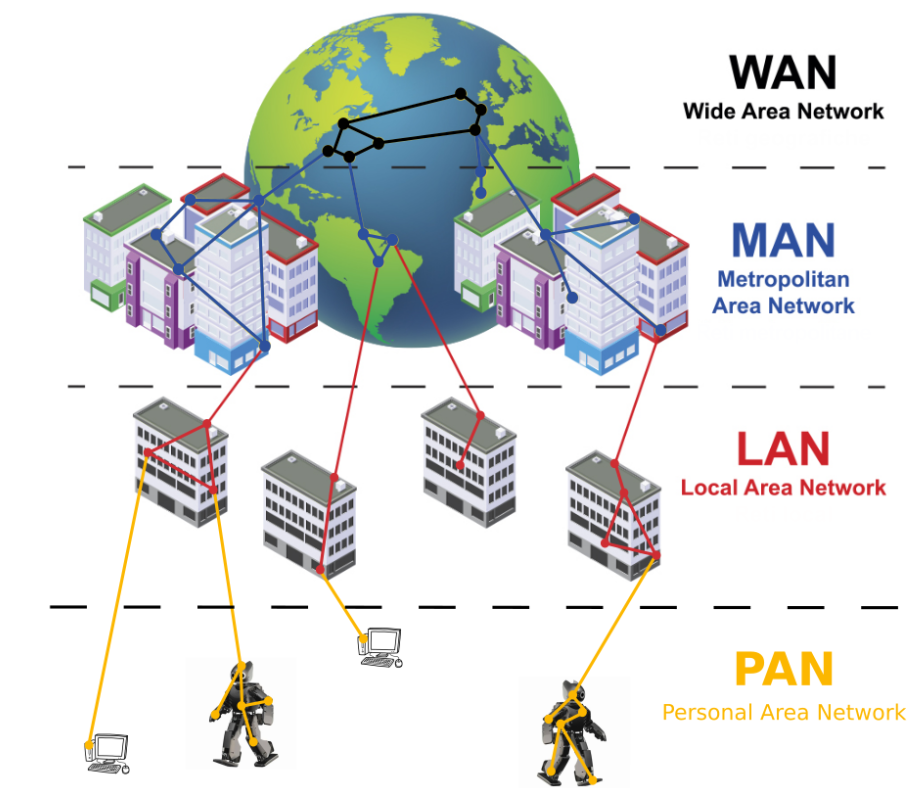
\includegraphics[width=5.35974in,height=4.63382in]{14-Logique/Cours/pandoc/media/image128.png}

\hypertarget{couches-du-moduxe8le-osi}{%
\subsubsection{Couches du modèle OSI}\label{couches-du-moduxe8le-osi}}

Le modèle OSI (de l'anglais open systems interconnection) est une norme de communica-\\
tion, en réseau, de tous les systèmes informatiques. C'est un modèle de communications entre\\
ordinateurs proposé par l'ISO (international organization for standardization) qui décrit les\\
fonctionnalités nécessaires à la communication et l'organisation de ces fonctions. Il norme l'organisation de l'architecture réseau en sept couches :

• 7. Application ;\\
• 6. Présentation ;\\
• 5. Session ;\\
• 4. Transport ;\\
• 3. Réseaux ;\\
• 2. Liaison ;\\
• 1. Physique.

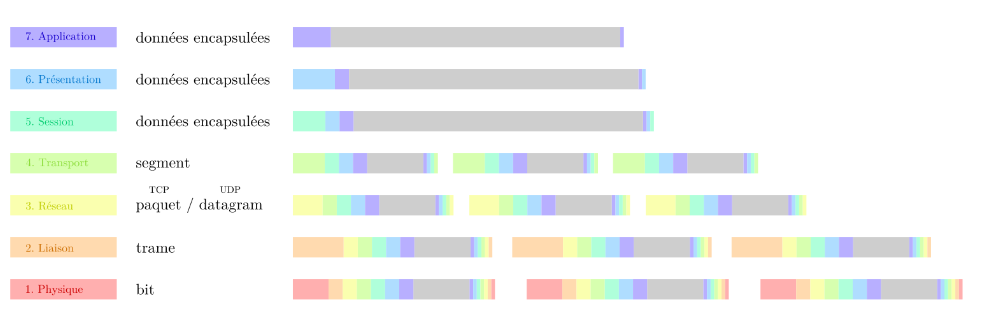
\includegraphics[width=6.90139in,height=2.17917in]{14-Logique/Cours/pandoc/media/image129.png}

On peut faire une métaphore entre la communication entre appareils informatiques et\\
entre humain. Dans les deux cas des règles sont mises en place. Par exemple, si vous voulez communiquer avec une personne, vous ne vous adresserez pas de la même manière s'il s'agit d'un parent, d'un enseignant, d'un camarade de classe ou d'un bébé.

\hypertarget{les-supports-de-transmission}{%
\subsubsection{Les supports de transmission}\label{les-supports-de-transmission}}

\hypertarget{caractuxe9ristiques-des-supports-de-transmission}{%
\subparagraph*{Caractéristiques des supports de transmission}\label{caractuxe9ristiques-des-supports-de-transmission}}
\addcontentsline{toc}{subparagraph}{Caractéristiques des supports de transmission}

On distingue les caractéristiques principales suivantes~:

\begin{itemize}
\item
  \textbf{Le taux d'erreur} : Rapport du nombre de bits émis erronés reçus au cours d'une période d'observation sur le nombre total de bits transmis pendant cette période.
\item
  \textbf{Le débit binaire} D exprimé en bit/s. Représente le nombre de bits transmis par seconde.
\item
  La rapidité de modulation R exprimée en Baud. Indique le nombre de symboles transmis par unité de temps.
\item
  \textbf{Bande Passante à -3 dB :} Plage de fréquence pour laquelle la puissance du signal de sortie est au pire divisée par 2 par rapport au signal d'entrée.
\item
  \textbf{Bruits et distorsions :} Même si les signaux sont transmis dans la bande passante du support, les signaux sont déformés (distorsions d'amplitude et/ou de phase). Des perturbations extérieures (foudre, champ électromagnétique, interférences, \ldots) peuvent également introduire des bruits.
\item
  \textbf{Capacité limite :} Quantité maximale d'information transportable par unité de temps.
\end{itemize}

\hypertarget{section-1}{%
\subparagraph*{}\label{section-1}}
\addcontentsline{toc}{subparagraph}{}

\hypertarget{les-diffuxe9rents-supports-de-transmission}{%
\subparagraph*{Les différents supports de transmission}\label{les-diffuxe9rents-supports-de-transmission}}
\addcontentsline{toc}{subparagraph}{Les différents supports de transmission}

Les supports de transmission peuvent être des câbles dans lesquels circulent des signaux électriques, l\textquotesingle atmosphère où circulent des ondes radio, ou des fibres optiques qui propagent des ondes lumineuses.

\begin{itemize}
\tightlist
\item
  
\includegraphics[width=2.27708in,height=0.98819in]{14-Logique/Cours/pandoc/media/image130.emf}\textbf{Le câble à paires torsadées} (et souvent blindées) : Les paires torsadées sont composées de 2 conducteurs en cuivre isolés l'un de l'autre et enroulés de façon hélicoïdale. Cela permet de réduire les influences électromagnétiques parasites provenant de l'environnement.
\end{itemize}

\begin{quote}
Le câble RJ45 couramment utilisé pour les réseaux ethernet est constitué de 4 paires torsadées.
\end{quote}

\emph{\ul{Utilisation :}} Liaisons téléphoniques, réseaux en étoile\ldots{}

\emph{\ul{Inconvénient :}} Atténuation importante

\emph{\ul{Débit maximal~:}} Jusqu'à 100Mbits/s (voire 1000Mbits/s pour certains câbles)

\begin{itemize}
\tightlist
\item
  \textbf{Les câbles coaxiaux} :
\end{itemize}

\begin{quote}

\includegraphics[width=3.15in,height=0.92834in]{14-Logique/Cours/pandoc/media/image131.emf}\emph{\ul{Utilisation :}} antennes TV\ldots{} Câbles remplacés par fibres optiques sur des longues distances.
\end{quote}

\emph{\ul{Débit maximal~:}} Plusieurs centaines de Mbits/s

\begin{quote}

\includegraphics[width=1.225in,height=0.81875in]{14-Logique/Cours/pandoc/media/image130.emf}
\end{quote}

\begin{itemize}
\tightlist
\item
  \textbf{L'atmosphère} : Utilisation des ondes électromagnétiques dans l'atmosphère ou le vide. Ce support comprend les faisceaux hertziens, les rayons infrarouges et les rayons laser.
\end{itemize}

\begin{quote}
Les ondes radio (radiofréquences 2,4 GHz) permettent de connecter des machines entre elles sans utiliser de câbles. La norme la plus utilisée actuellement pour les réseaux sans fil est la norme IEEE 802.11, mieux connue sous le nom de Wi-Fi. Le Wi-Fi permet de relier des machines à une liaison haut débit (plusieurs dizaines de Mbits/s) sur un rayon de plusieurs dizaines de mètres en intérieur (plusieurs centaines de mètres en extérieur).
\end{quote}

\emph{\ul{Avantage :}} Pas de support physique

\begin{quote}
\emph{\ul{Inconvénients :}} Conditions météorologiques, confidentialité
\end{quote}

\emph{\ul{Débit maximal~:}} Plusieurs dizaines de Mbits/s (Plusieurs centaines de Mbit/s avec certains matériels)


\includegraphics[width=4.15833in,height=2.20833in]{14-Logique/Cours/pandoc/media/image132.emf}


\includegraphics[width=0.71875in,height=0.95833in]{14-Logique/Cours/pandoc/media/image130.emf}

\begin{itemize}
\tightlist
\item
  \textbf{La fibre optique} : Constituée d'un fil de verre très fin. Le coeur de la fibre propage la lumière.
\end{itemize}

\begin{quote}
La fibre optique autorise des vitesses de communication très élevées (plus de 100 Gigabit/s) ou en milieu très fortement parasité.


\includegraphics[width=2.39792in,height=1.05in]{14-Logique/Cours/pandoc/media/image133.emf}

\emph{\ul{Avantages :}} masse linéique très faible, BP immense (30 THz), faible atténuation, insensibilité aux parasites électromagnétiques, \ldots{}
\end{quote}

\emph{\ul{Inconvénients :}} Prix de la fibre, prix des modulateurs, mode de pose.

\emph{\ul{Débit maximal~:}} 1 à 100 Gbits/s

\begin{itemize}
\tightlist
\item
  
\includegraphics[width=1.28681in,height=1.24653in]{14-Logique/Cours/pandoc/media/image134.emf}
\includegraphics[width=2.56458in,height=1.2625in]{14-Logique/Cours/pandoc/media/image135.emf}\textbf{La liaison CPL (Courants Porteurs en Ligne)~:} il s'agit d'une technique permettant le transfert d\textquotesingle informations numériques en passant par les lignes électriques. La technologie CPL superpose un signal à hautes fréquences au signal électrique classique (50Hz, 23V). Le signal est reçu par tout boitier se trouvant dans le même circuit électrique.
\end{itemize}

\begin{quote}

\includegraphics[width=2.05in,height=2.5125in]{14-Logique/Cours/pandoc/media/image136.emf}

Il est bien sûr possible de mixer le CPL avec d\textquotesingle autres supports de transmission, comme le montre le schéma ci-contre :
\end{quote}

\emph{\ul{Débit maximal~:}} 200 à 2000 Mbits/s

\begin{quote}
Par défaut, l\textquotesingle installation de boitier CPL ne nécessite aucune configuration ni programme.

Cependant, si on veut sécuriser quelque peu le réseau CPL, on utilise un outil spécifique qui permet de donner un nom au réseau CPL. Ce nom permet de rendre ce réseau invisible aux autres boitiers.
\end{quote}

\hypertarget{principemultiplexagemultiplexage}{%
\subsubsection[Multiplexage]{\texorpdfstring{\protect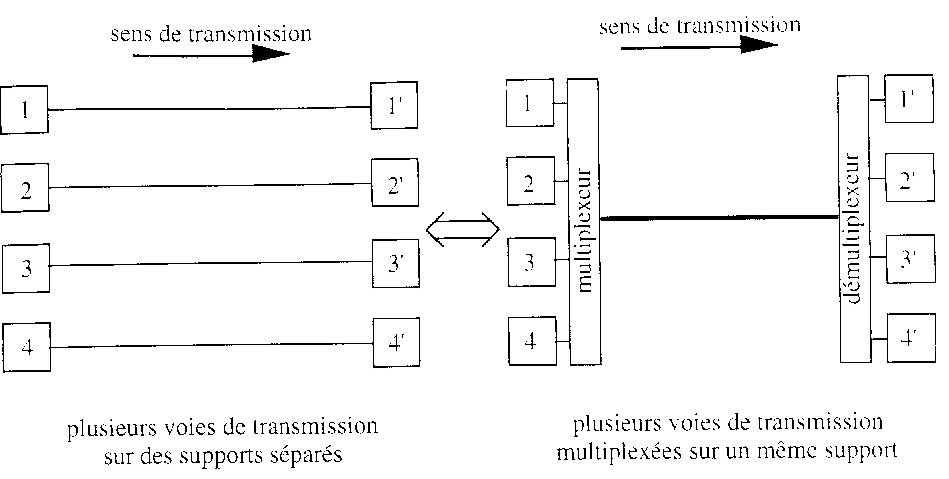
\includegraphics[width=4.625in,height=2.14931in]{14-Logique/Cours/pandoc/media/image137.jpeg}Multiplexage}{principemultiplexageMultiplexage}}\label{principemultiplexagemultiplexage}}

Lorsque la bande passante d'un support physique est nettement supérieure au spectre du signal à émettre, il est intéressant d'utiliser ce même support pour transmettre plusieurs signaux. On parle alors de MULTIPLEXAGE.

2 possibilités :

\begin{itemize}
\tightlist
\item
  Multiplexage fréquentiel;
\end{itemize}

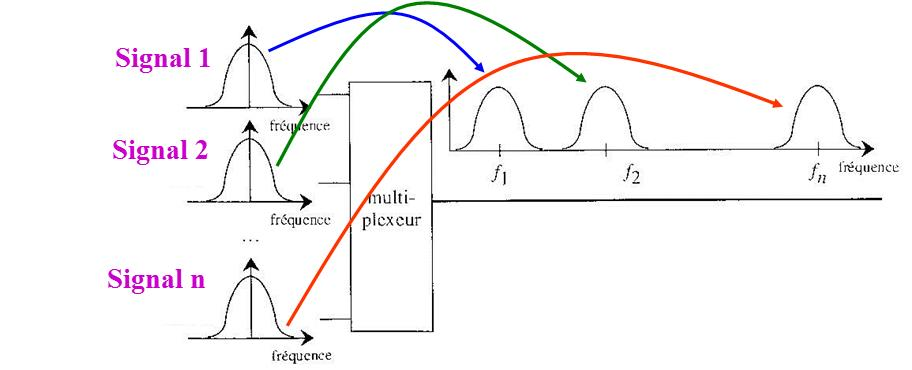
\includegraphics[width=4.80208in,height=2.18333in]{14-Logique/Cours/pandoc/media/image138.jpeg}

\ul{Principe :} On découpe la bande passante du support en plusieurs sous bandes. Chaque sous bande est affectée à une voie de transmission.

Chaque signal d'entrée est modulé en fréquence. La voie n est modulée par une porteuse à la fréquence f\textsubscript{n}.

Dans ce cas, le multiplexeur joue le rôle d'un additionneur de n signaux à différentes fréquences.

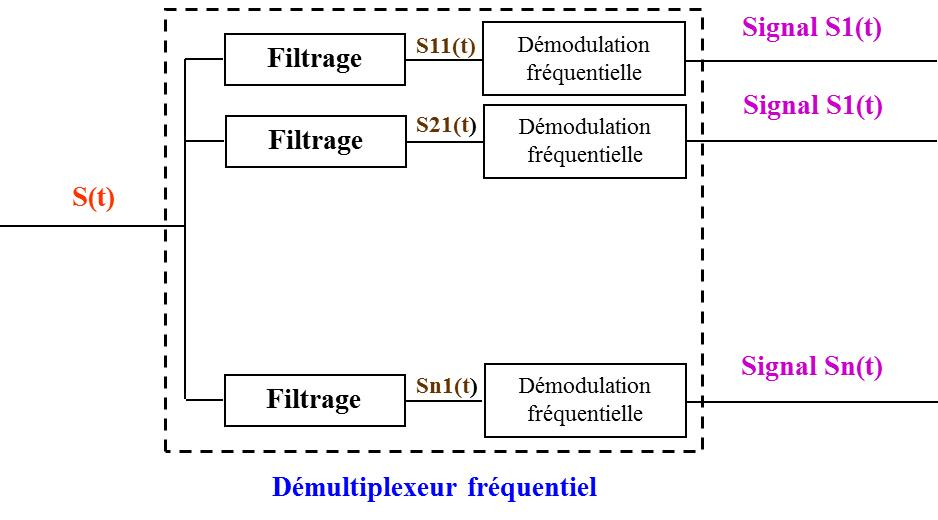
\includegraphics[width=3.28681in,height=1.82222in]{14-Logique/Cours/pandoc/media/image139.jpeg}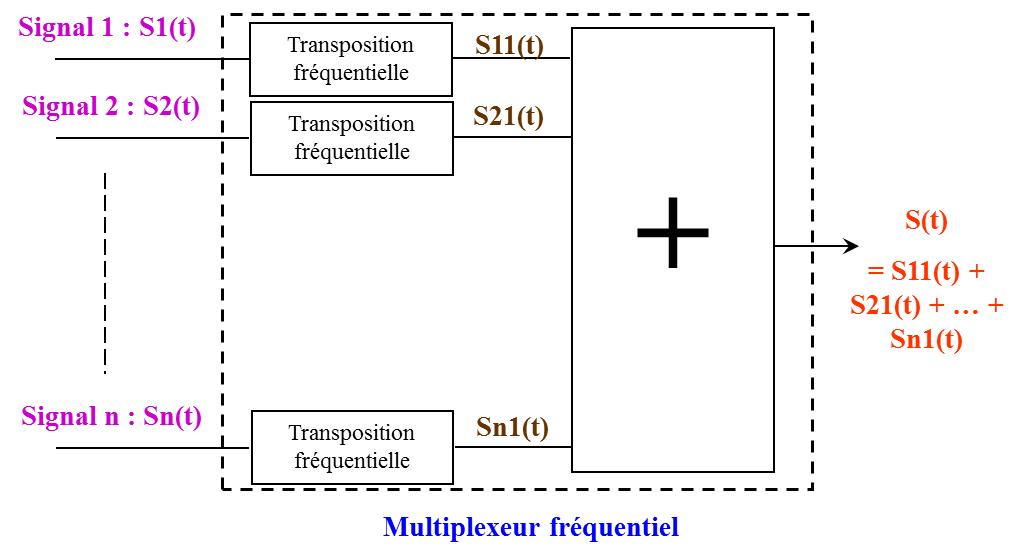
\includegraphics[width=3.89653in,height=2.12222in]{14-Logique/Cours/pandoc/media/image140.jpeg}A la réception, on filtre le signal reçu S(t) par des filtres passe bande qui récupère les signaux Si1(t), et après une démodulation de fréquence, on réobtient les signaux originaux Si(t).

\begin{itemize}
\tightlist
\item
  Multiplexage temporel.
\end{itemize}

\hypertarget{les-erreurs-de-transmission}{%
\subsubsection{Les erreurs de transmission}\label{les-erreurs-de-transmission}}

Entre les deux extrémités d'une liaison, la présence des imperfections du support de transmission (affaiblissement, déphasage), et la présence de bruit électromagnétique, perturbent de façon aléatoire les données transmises. Ces perturbations se traduisent au niveau de l'information reçue, par des modifications : soit des disparitions, soit des adjonctions, soit des inversions (0 en 1 ou 1 en 0).

L'objet de cette partie, est d'aborder les méthodes couramment utilisées dans les réseaux informatiques, pour protéger les données émises contre les erreurs introduites par le canal de transmission.


\includegraphics[width=4.95972in,height=1.00972in]{14-Logique/Cours/pandoc/media/image141.emf}Ces techniques utilisent un codeur à l'émission et un décodeur à la réception, comme le montre la figure ci-contre.

La technique adoptée dans la plupart des systèmes de détection d'erreurs, consiste à ajouter des bits supplémentaires (dit redondants) à chaque bloc de données avant de le transmettre sur le support de transmission.

\hypertarget{section-2}{%
\subparagraph*{}\label{section-2}}
\addcontentsline{toc}{subparagraph}{}

\hypertarget{contruxf4le-de-parituxe9-lrc}{%
\subparagraph*{Contrôle de parité (LRC)}\label{contruxf4le-de-parituxe9-lrc}}
\addcontentsline{toc}{subparagraph}{Contrôle de parité (LRC)}

Le contrôle de parité est aussi appelé LRC (Longitudinal Redundancy Check).

Il existe deux types de contrôle de parité (pair et impair) et il est indispensable que l'émetteur et le récepteur s'entendent sur le type à utiliser pour l'ensemble de la transmission.

\textbf{Parité paire :} Lorsque le nombre de «~1~» dans les données envoyées est impair, le bit de parité (bit de contrôle) est placé à «~1~» de manière à ce que le nombre total de «~1~» soit pair y compris le bit de parité. Dans le cas contraire, le bit de parité est placé à «~0~».


\includegraphics[width=5.07083in,height=0.65208in]{14-Logique/Cours/pandoc/media/image142.emf}

\textbf{Parité impaire :} Elle correspond au système inverse.

Quelle que soit la parité choisie, si un bit est modifié au cours de la transmission, les calculs de parité effectués par l'émetteur et par le récepteur différeront.

Cette méthode est peu performante, le contrôle fonctionne correctement seulement si le nombre de bits modifiés est impair.

Si on met cela sous forme d'équation logique, le ou exclusif est très utile.

\[Bp_{paire} = \overset{\underset{n}{i = 1}}{\oplus}d_{i}\ \ \ \ \ \ \ \ \ \ \ \ \ \ \ \ \ \ \ \ \ \ \ \ \ \ \ \ \ \ \ Bp_{impaire} = \overline{\overset{\underset{n}{i = 1}}{\oplus}d_{i}}\]

\begin{longtable}[]{@{}
  >{\raggedright\arraybackslash}p{(\columnwidth - 2\tabcolsep) * \real{0.1250}}
  >{\raggedright\arraybackslash}p{(\columnwidth - 2\tabcolsep) * \real{0.8611}}@{}}
\toprule\noalign{}
\begin{minipage}[b]{\linewidth}\raggedright
\begin{quote}
{[}{]} (14-Lo gique/ Cours/ pandoc /media /image 10.png )\{widt h=``0.6 262696 850393 701in''

height =``0.65 083333 333333 34in''\}
\end{quote}
\end{minipage} & \begin{minipage}[b]{\linewidth}\raggedright
\textbf{Exemples}

\textbf{Parité paire~:}

\textbf{Quelle doit être le bit de parité pour la donnée suivante~:}

11001011

La donnée contenant 5 état 1, le bit de parité paire est positionné à 1,\\
ramenant ainsi le nombre de 1 à 6.

\textbf{Parité impaire~:}

\textbf{Quelle doit être le bit de parité pour la donnée suivante~:}

11001011

La donnée contenant 5 état 1, le bit de parité paire est positionné à 0,\\
laissant ainsi un nombre de 1 impaire\strut
\end{minipage} \\
\midrule\noalign{}
\endhead
\bottomrule\noalign{}
\endlastfoot
& \\
\end{longtable}

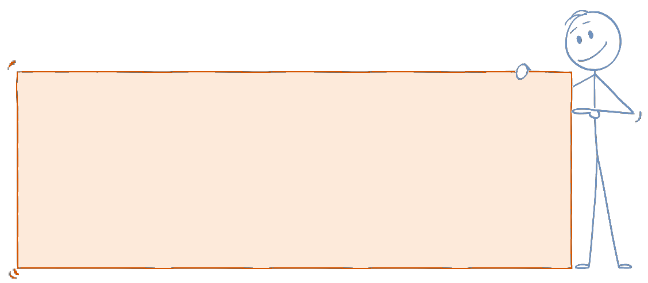
\includegraphics[width=4.73333in,height=1.83333in]{14-Logique/Cours/pandoc/media/image8.png}

\hypertarget{contruxf4le-de-redondance-cyclique-crc}{%
\subparagraph*{Contrôle de Redondance cyclique (CRC)}\label{contruxf4le-de-redondance-cyclique-crc}}
\addcontentsline{toc}{subparagraph}{Contrôle de Redondance cyclique (CRC)}


\includegraphics[width=3.19583in,height=0.61736in]{14-Logique/Cours/pandoc/media/image143.emf}La méthode de détection d'erreurs appelée CRC (Cyclic Redundancy Check) permet de détecter plus d'erreurs que le contrôle de parité. Elle nécessite l'ajout de bits redondants r\textsubscript{0} à r\textsubscript{k}, calculés à partir des données a\textsubscript{0} à a\textsubscript{n}. Les polynômes CRC ou FCS qui utilisent les bits r\textsubscript{0} à r\textsubscript{k} sont établis à partir de normes.

\ul{Exemple :} 3 octets à transmettre

1 1 0 0 1 1 0 0

+ 1 0 1 1 0 0 1 0

+ 0 1 0 0 1 1 0 1

0 0 1 1 0 0 1 1

On fait une addition binaire Modulo 2 entre chaque bit sans retenue.

Par contrôle polynomial (par abus de langage CRC=Cyclic Redundancy Check) :

\begin{longtable}[]{@{}
  >{\raggedright\arraybackslash}p{(\columnwidth - 16\tabcolsep) * \real{0.1169}}
  >{\raggedright\arraybackslash}p{(\columnwidth - 16\tabcolsep) * \real{0.1169}}
  >{\raggedright\arraybackslash}p{(\columnwidth - 16\tabcolsep) * \real{0.1169}}
  >{\raggedright\arraybackslash}p{(\columnwidth - 16\tabcolsep) * \real{0.1039}}
  >{\raggedright\arraybackslash}p{(\columnwidth - 16\tabcolsep) * \real{0.1039}}
  >{\raggedright\arraybackslash}p{(\columnwidth - 16\tabcolsep) * \real{0.1039}}
  >{\raggedright\arraybackslash}p{(\columnwidth - 16\tabcolsep) * \real{0.1039}}
  >{\raggedright\arraybackslash}p{(\columnwidth - 16\tabcolsep) * \real{0.1039}}
  >{\raggedright\arraybackslash}p{(\columnwidth - 16\tabcolsep) * \real{0.1039}}@{}}
\toprule\noalign{}
\endhead
\bottomrule\noalign{}
\endlastfoot
a\textsubscript{n-1} & a\textsubscript{n-2} & a\textsubscript{n-3} & \ldots{} & \ldots{} & \ldots{} & \ldots{} & a\textsubscript{1} & a\textsubscript{0} \\
\end{longtable}

On considère la trame à transmettre comme un groupe de bits. On lui associe un polynôme P(X) tel que le coefficient de degré i corresponde à la valeur du i\textsuperscript{ème} bit.

\[P(X) = \sum_{k = 0}^{n - 1}{a_{k}.X^{k}}\]

On choisit un polynôme appelé polynôme générateur G(X) de degré « r » ayant des propriétés spécifiques.

On calcule X\textsuperscript{r}*P(X) et on le divise par G(X). Le reste de cette division polynomiale est un autre polynôme noté R(X).

On transmet :

\begin{longtable}[]{@{}
  >{\raggedright\arraybackslash}p{(\columnwidth - 18\tabcolsep) * \real{0.1059}}
  >{\raggedright\arraybackslash}p{(\columnwidth - 18\tabcolsep) * \real{0.1059}}
  >{\raggedright\arraybackslash}p{(\columnwidth - 18\tabcolsep) * \real{0.1059}}
  >{\raggedright\arraybackslash}p{(\columnwidth - 18\tabcolsep) * \real{0.0941}}
  >{\raggedright\arraybackslash}p{(\columnwidth - 18\tabcolsep) * \real{0.0941}}
  >{\raggedright\arraybackslash}p{(\columnwidth - 18\tabcolsep) * \real{0.0941}}
  >{\raggedright\arraybackslash}p{(\columnwidth - 18\tabcolsep) * \real{0.0941}}
  >{\raggedright\arraybackslash}p{(\columnwidth - 18\tabcolsep) * \real{0.0941}}
  >{\raggedright\arraybackslash}p{(\columnwidth - 18\tabcolsep) * \real{0.0941}}
  >{\raggedright\arraybackslash}p{(\columnwidth - 18\tabcolsep) * \real{0.0941}}@{}}
\toprule\noalign{}
\endhead
\bottomrule\noalign{}
\endlastfoot
a\textsubscript{n-1} & a\textsubscript{n-2} & a\textsubscript{n-3} & \ldots{} & a\textsubscript{1} & a\textsubscript{0} & r\textsubscript{k} & \ldots{} & r\textsubscript{1} & r\textsubscript{0} \\
\end{longtable}

A la réception, on vérifie que le reste de la division par G(X) est nul.

\ul{Exemple :}

\begin{longtable}[]{@{}
  >{\raggedright\arraybackslash}p{(\columnwidth - 2\tabcolsep) * \real{0.1250}}
  >{\raggedright\arraybackslash}p{(\columnwidth - 2\tabcolsep) * \real{0.8611}}@{}}
\toprule\noalign{}
\begin{minipage}[b]{\linewidth}\raggedright
\begin{quote}
{[}{]} (14-Lo gique/ Cours/ pandoc /media /image 10.png )\{widt h=``0.6 262696 850393 701in''

height =``0.65 083333 333333 34in''\}
\end{quote}
\end{minipage} & \begin{minipage}[b]{\linewidth}\raggedright
\textbf{Exemples}

Soit la séquence 1001 à envoyer ;

Le polynôme P(X) vaut donc X\textsuperscript{3}+1;

Si le polynôme générateur est G(X)=X\textsuperscript{3}+X+1, le degré de G(x) est r=3;

Par conséquent P(X).X\textsuperscript{3} vaut X\textsuperscript{6}+X
\end{minipage} \\
\midrule\noalign{}
\endhead
\bottomrule\noalign{}
\endlastfoot
& \\
\end{longtable}

\hypertarget{section-3}{%
\subparagraph*{}\label{section-3}}
\addcontentsline{toc}{subparagraph}{}

\hypertarget{accusuxe9-de-ruxe9ception}{%
\subparagraph*{Accusé de réception}\label{accusuxe9-de-ruxe9ception}}
\addcontentsline{toc}{subparagraph}{Accusé de réception}

La détection d'erreur suivie d'une retransmission est la solution la plus utilisée dans les réseaux informatiques.

Des mécanismes d'accusés de réception (ACKnowledge acquittements) sous la forme de blocs de données spéciaux permettent de confirmer à l'émetteur que les données transmises sont bien arrivées sans erreur.

\hypertarget{notion-de-taux-derreurs}{%
\subparagraph*{Notion de taux d'erreurs}\label{notion-de-taux-derreurs}}
\addcontentsline{toc}{subparagraph}{Notion de taux d'erreurs}

Dans la pratique, on mesure la qualité d'une liaison numérique (qualité de transmission) par le taux d'erreur appelée BER (Bit Error Rate), il est donné par le nombre de bits erronés rapporté au nombre total de bit transmis.

Le taux d'erreurs varie en pratique de 10\textsuperscript{-4} (ligne téléphonique) à 10\textsuperscript{-9} (réseaux locaux).

Le taux d'erreurs est devenu très satisfaisant descendant souvent sous la barre des 10\textsuperscript{-9}~: cela provient de techniques de codage plus performantes et de l'utilisation de support de transmission de très bonnes qualités comme la fibre optique

\hypertarget{topologie-des-ruxe9seaux}{%
\subsubsection{Topologie des réseaux}\label{topologie-des-ruxe9seaux}}

La \textbf{topologie c'est l'organisation physique d'un réseau}. Pour résumer, elle permet de savoir comment sont raccordés tous les éléments pouvant communiquer entre eux ?

\begin{figure}
\centering
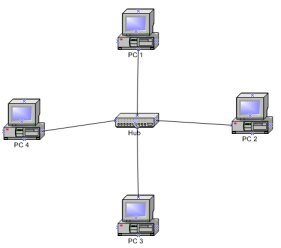
\includegraphics[width=1.825in,height=1.61111in]{14-Logique/Cours/pandoc/media/image144.jpeg}
\caption{etoile}
\end{figure}

\textbf{Topologie en étoile}

C'est la topologie la plus courante. Toutes les stations sont reliées à un unique composant central : le concentrateur (hub). Quand une station émet vers le concentrateur (qui peut être un switch ou un hub), celui-ci envoie les données à celle qui en est le destinataire (switch) ou à toutes les autres machines (hub).

\begin{quote}
\textbf{Avantages / Inconvénients}

Ce type de réseau est facile à mettre en place et à surveiller. La panne d'une station ne met pas en cause l'ensemble du réseau. Par contre, il faut plus de câbles que pour les autres topologies, et si le concentrateur tombe en panne, tout le réseau est hors d'état de fonctionner. De plus, le débit utile de circulation de données est moins bon que pour les autres topologies.
\end{quote}

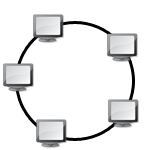
\includegraphics[width=1.87361in,height=1.87361in]{14-Logique/Cours/pandoc/media/image145.png}\\
\textbf{Topologie en anneau}

Développée par IBM, cette architecture est principalement utilisée par les réseaux Token-Ring 1. Elle utilise la technique d'accès par ``jeton''. Les informations circulent de station en\\
station, en suivant l'anneau. Un jeton circule autour de l'anneau. La station qui a le jeton émet des données qui font le tour de l'anneau. Lorsque les données reviennent, la station qui les a envoyées les élimine du réseau et passe le jeton à son voisin, et ainsi de suite...

\begin{quote}
\textbf{Avantages / Inconvénients}

Cette topologie permet d'avoir un débit proche de 90\% de la bande passante (capacité à transporter un type d'information dans un canal). De plus, le signal qui circule est régénéré par chaque station. En réalité les ordinateurs d'un réseau en anneau ne sont pas reliés en boucle, mais sont reliés à un répartiteur (appelé MAU, Multistation Access Unit) qui va gérer la communication entre les ordinateurs qui lui sont reliés en impartissant à chacun d'entre eux un temps de parole.
\end{quote}

\hypertarget{topologie-en-bus}{%
\subparagraph*{Topologie en bus}\label{topologie-en-bus}}
\addcontentsline{toc}{subparagraph}{Topologie en bus}

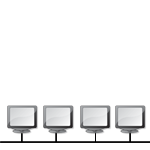
\includegraphics[width=2.09097in,height=0.74792in]{14-Logique/Cours/pandoc/media/image146.png}Le bus est un segment central où circulent les informations. Il s'étend sur toute la longueur du réseau et les machines viennent s'y connecter. Lorsqu'une station émet des données, elles circulent sur toute la longueur du bus et la station destinatrice peut les récupérer. Une seule station peut émettre à la fois. En bout de bus, un ``bouchon'' permet de supprimer définitivement les informations pour qu'une autre station puisse émettre.

\begin{quote}
\textbf{Avantages / Inconvénients}

L'avantage du bus réside dans la simplicité de sa mise en œuvre. Par contre, en cas de rupture de la structure bus, le réseau devient inutilisable. Notons également que le signal n'est jamais régénéré, ce qui limite la longueur des câbles (car plus un signal électrique parcours un câble métallique, plus son amplitude diminue).
\end{quote}

\hypertarget{mailleetopologie-mailluxe9e}{%
\subparagraph*{\texorpdfstring{\protect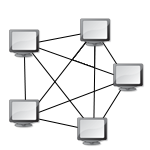
\includegraphics[width=1.92222in,height=1.71736in]{14-Logique/Cours/pandoc/media/image147.png}Topologie maillée}{mailleeTopologie maillée}}\label{mailleetopologie-mailluxe9e}}
\addcontentsline{toc}{subparagraph}{Topologie maillée}

La topologie maillée (c.f. Figure 3.4) est une évolution de la topologie en étoile. Très utilisée dans les très grands réseaux, elle permet d'offrir des chemins différents pour relier\\
deux points, ce qui évite les problèmes en cas de rupture d'une liaison.

\begin{quote}
\textbf{Avantages / Inconvénients}

L'avantage de la structure maillée est que la topologie est robuste et sûre. Par contre, les coûts de mise en place sont importants.
\end{quote}

\hypertarget{types-de-liaisons-des-ruxe9seaux-de-communication}{%
\subsubsection{Types de liaisons des réseaux de communication}\label{types-de-liaisons-des-ruxe9seaux-de-communication}}

Au sein d'un réseau local, on distingue deux modes de fonctionnement (c.f. Figure 3.5) :\\
• Liaison client-serveur (server based network) : elle désigne un mode de communication\\
à travers un réseau entre un client (logiciel implémenté sur un ordinateur) qui envoie\\
des requêtes 2, et un serveur qui attend les requêtes et y répond ;\\
• Liaison point à point (peer to peer) : Ce mode est adapté pour les liaisons simples\\
qui transportent des données entre deux matériels homologues. Cette liaison permet un\\
fonctionnement bidirectionnel simultané.

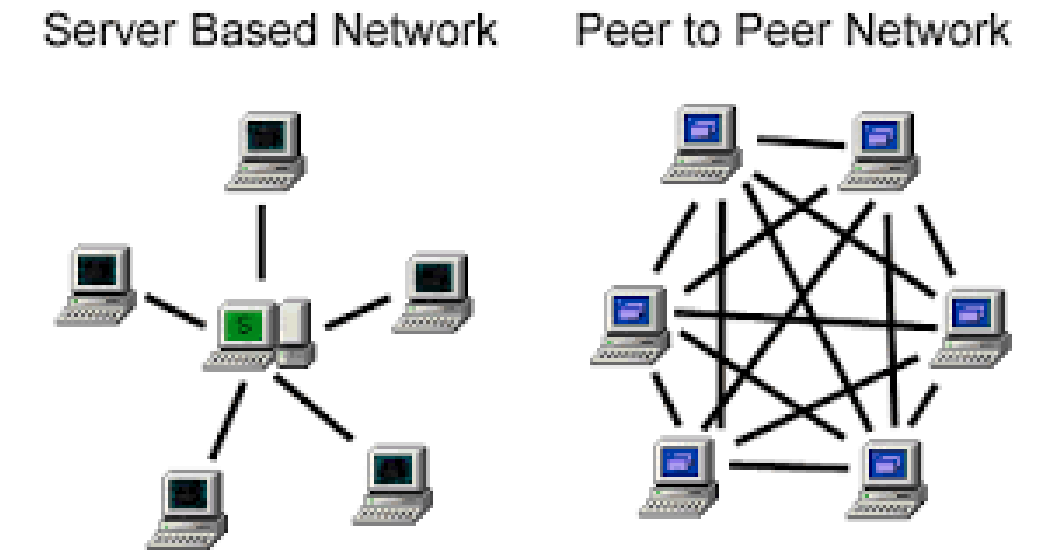
\includegraphics[width=3.97184in,height=2.09702in]{14-Logique/Cours/pandoc/media/image148.png}

\hypertarget{architecture-de-la-chauxeene-de-transmission}{%
\subsubsection{Architecture de la chaîne de transmission}\label{architecture-de-la-chauxeene-de-transmission}}


\includegraphics[width=5.98333in,height=2.25833in]{14-Logique/Cours/pandoc/media/image149.emf}

La \textbf{source} est l'équipement qui génère les données à transmettre (Ordinateur, \ldots)

L'\textbf{émetteur} reçoit en entrée la suite de données binaires ou un signal analogique et fournit en sortie un signal dont les caractéristiques sont adaptées au support de transmission (adaptation en tension, courant, optique\ldots)

Le \textbf{récepteur} réalise la fonction inverse pour donner le message au \textbf{destinataire}.

Pour une transmission sur une voie de communication entre deux machines, la communication peut s\textquotesingle effectuer de différentes manières. La transmission est caractérisée par :

\begin{itemize}
\item
  le modes de transmission
\item
  le sens des échanges
\item
  la synchronisation : synchrone ou asynchrone
\item
  le protocole de communication utilisé
\end{itemize}

\begin{quote}
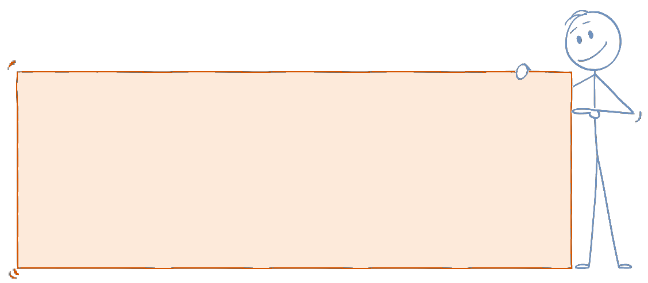
\includegraphics[width=5.89815in,height=2.75in]{14-Logique/Cours/pandoc/media/image8.png}
\end{quote}

\hypertarget{caractuxe9ristiques-de-la-transmission}{%
\subsubsection{Caractéristiques de la transmission}\label{caractuxe9ristiques-de-la-transmission}}

Pour une transmission sur une voie de communication entre deux machines, la communication peut s\textquotesingle effectuer de différentes manières. La transmission est caractérisée par~:

\begin{itemize}
\tightlist
\item
  le \textbf{sens des échanges};
\end{itemize}

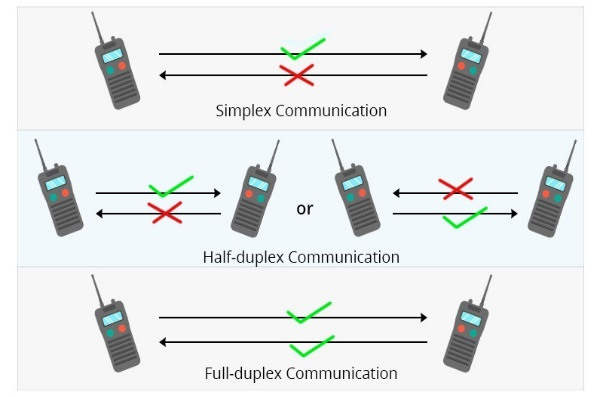
\includegraphics[width=2.73958in,height=1.80347in]{14-Logique/Cours/pandoc/media/image150.jpeg}Pour une transmission entre deux points, la plupart du temps, il faut traiter un dialogue et non un monologue. Il faut donc une convention pour fixer le sens de la transmission.

\begin{itemize}
\item
  Dans un seul sens~: liaison \textbf{simplex}
\item
  Dans les deux sens non simultanément~: liaison \textbf{half duplex}
\item
  Dans les deux sens simultanément~: liaison \textbf{full duplex} ou \textbf{duplex intégral}
\end{itemize}

\begin{figure}
\centering
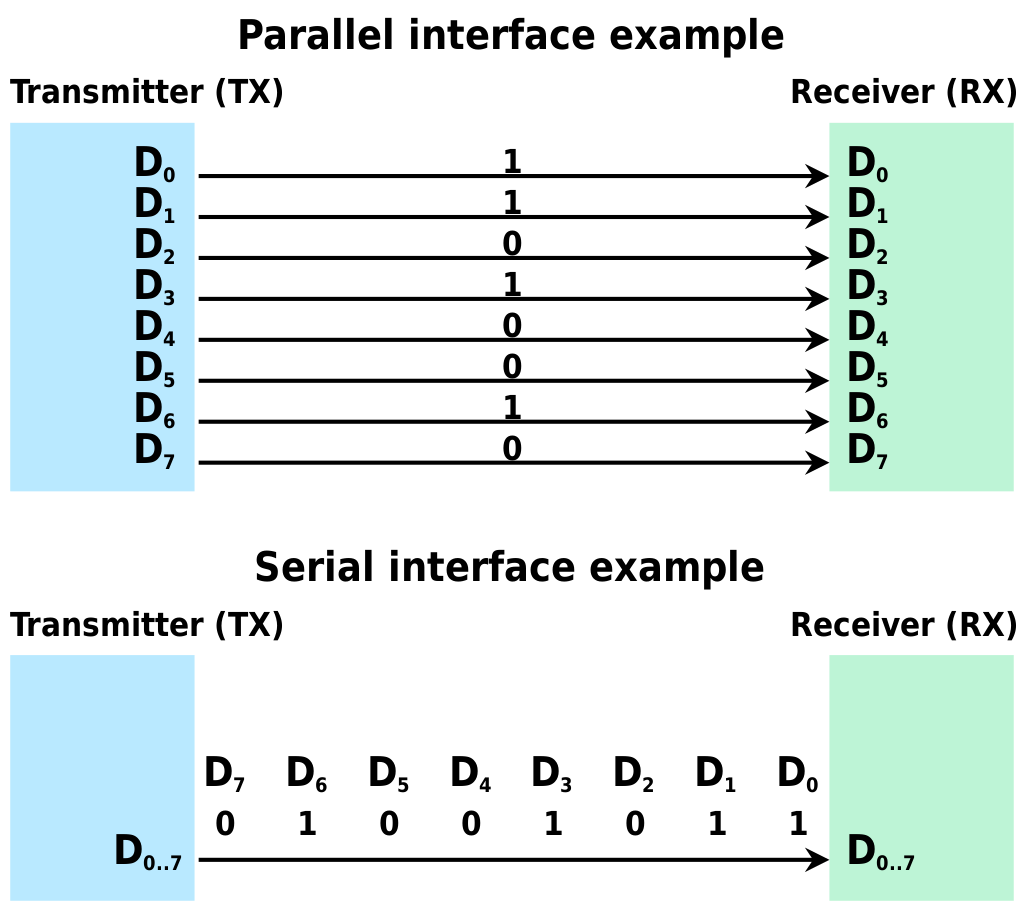
\includegraphics[width=3.17917in,height=2.82824in]{14-Logique/Cours/pandoc/media/image151.png}
\caption{undefined}
\end{figure}

\begin{itemize}
\item
  le mode de transmission : \textbf{série ou parallèle};

  \begin{itemize}
  \item
    Lors d'une liaison parallèle, chaque BIT est transmis sur un fil, (rapide mais consommateur de fil)
  \item
    Pour une liaison série, les bits sont transmis les uns après les autres, (lent mais moins consommateur de fils).
  \end{itemize}
\item
  la synchronisation : \textbf{synchrone ou asynchrone}.
\end{itemize}

\begin{quote}
\textbf{Liaison asynchrone} : Chaque caractère est émis de façon irrégulière dans le temps Imaginons qu\textquotesingle un seul bit soit transmis pendant une longue période de silence. Le récepteur ne pourrait savoir s\textquotesingle il s\textquotesingle agit de 00010000, ou 10000000 ou encore 00000100...

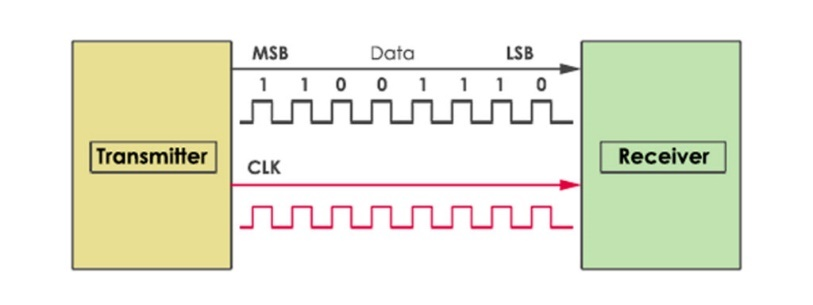
\includegraphics[width=3.69444in,height=1.38551in]{14-Logique/Cours/pandoc/media/image152.jpeg}\textbf{Liaison synchrone} : Emetteur et Récepteur sont cadencés à la même horloge (CLK). Le récepteur reçoit de façon continue les informations au rythme où l\textquotesingle émetteur les envoie.
\end{quote}

\hypertarget{protocoles-des-ruxe9seaux-de-communication}{%
\subsubsection{Protocoles des réseaux de communication}\label{protocoles-des-ruxe9seaux-de-communication}}

Les réseaux utilisent une architecture en couches, dans laquelle la communication entre\\
les appareils obéit à des règles précises définies par des protocoles de communication. Les\\
informations pouvant être altérées durant le transport, il faut superviser la circulation des\\
données. Le protocole spécifie le format des unités de données échangées, leur délimitation, les moyens de contrôler leur validité ainsi que le mode de correction des erreurs détectées.

Les données sont encapsulées, puis scindées en paquets. La petite taille des paquets permet de réduire le délai global d'acheminement des messages. Ces paquets sont ensuite adaptés au type d'appareil avec lequel on veut communiquer, on appelle alors cet élément une trame. Cette trame est finalement convertie en un signal physique adapté au support de communication (câble métallique, air, fibre optique). Voici un exemple d'encapsulation de données, qui donne une trame.

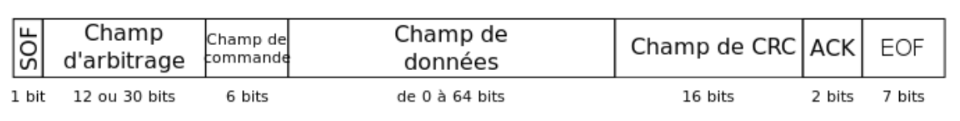
\includegraphics[width=6.90139in,height=0.87014in]{14-Logique/Cours/pandoc/media/image153.png}

Un protocole est donc un ensemble de règles régissant les échanges de données entre\\
équipements informatiques. Pour qu'un message soit correctement reçu et interprété il faut respecter quelques règles :

- s'adresser au bon destinataire, (adresse)

- lui indiquer que la communication débute, (bit de start)

- parler la même « langue » etc... (même débit, même codage,\ldots)

En format simplifié, cela donnerait~:

\begin{longtable}[]{@{}
  >{\raggedright\arraybackslash}p{(\columnwidth - 4\tabcolsep) * \real{0.1818}}
  >{\raggedright\arraybackslash}p{(\columnwidth - 4\tabcolsep) * \real{0.4935}}
  >{\raggedright\arraybackslash}p{(\columnwidth - 4\tabcolsep) * \real{0.2987}}@{}}
\toprule\noalign{}
\endhead
\bottomrule\noalign{}
\endlastfoot
\textbf{En-tête} & \textbf{Données applicatives} & \textbf{Terminateur} \\
\end{longtable}

Ce qui est vrai pour nous l'est également pour les machines. Une information ne sera donc jamais envoyée seule mais sera toujours précédée et terminée par des données (binaires) dites « de service ». Celles qui précédent l'information à transmettre (donnée(s) applicative(s)) constituent l'en-tête, celles qui la suivent correspondent au terminateur.

Définir un protocole de liaison de données consiste notamment à préciser :

\begin{itemize}
\item
  le format des trames (nombre de bit total d'une trame);
\item
  le critère de début et de fin de trame;
\item
  la place et la signification des différents champs dans une trame;
\item
  la technique de détection d'erreur utilisée;
\item
  les règles de dialogue : procédure après détection d'erreur, règle de priorité, \ldots{}
\end{itemize}

\hypertarget{codage}{%
\subparagraph*{Codage}\label{codage}}
\addcontentsline{toc}{subparagraph}{Codage}

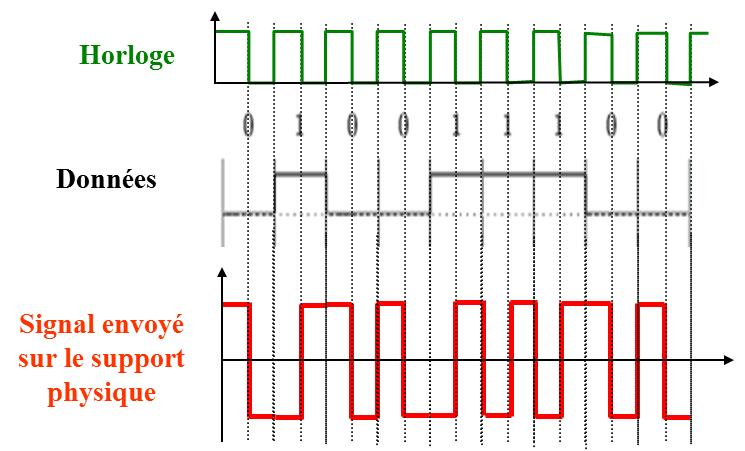
\includegraphics[width=4.12569in,height=2.29444in]{14-Logique/Cours/pandoc/media/image154.jpeg}\textbf{Code de MANCHESTER} : Il introduit une transition au milieu de chaque intervalle.

Il consiste en fait à faire un OU exclusif entre le signal et le signal d\textquotesingle horloge. Ce qui se traduit par un front montant lorsque le bit est à zéro, un front descendant dans le cas contraire.

On envoie les bits en série à chaque front montant de l'horloge.

\textbf{Code de MILLER} : Identique au code de MANCHESTER, à ceci près qu\textquotesingle une transition apparaît au milieu de l\textquotesingle intervalle alternativement uniquement lorsque le bit est à 1. De plus, pour éviter les longues suites de 0 posant toujours un problème lors de la synchronisation à la réception, si un bit 0 est suivi d'un autre 0, on rajoute une transition à la fin du temps d'horloge.

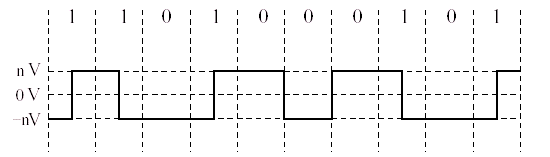
\includegraphics[width=4.53262in,height=1.29386in]{14-Logique/Cours/pandoc/media/image155.png}

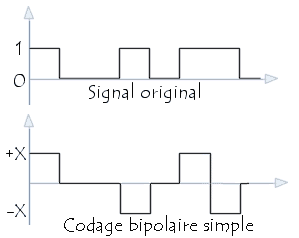
\includegraphics[width=2.59514in,height=2.06528in]{14-Logique/Cours/pandoc/media/image156.png}\textbf{Code bipolaire simple} : Codage sur trois niveaux.

Il propose trois états de la grandeur transportée sur le support physique~:

\begin{itemize}
\item
  La valeur 0 lorsque le bit est à 0
\item
  Alternativement +X et -X lorsque le bit est à 1
\end{itemize}

\begin{longtable}[]{@{}
  >{\raggedright\arraybackslash}p{(\columnwidth - 2\tabcolsep) * \real{0.1250}}
  >{\raggedright\arraybackslash}p{(\columnwidth - 2\tabcolsep) * \real{0.8611}}@{}}
\toprule\noalign{}
\begin{minipage}[b]{\linewidth}\raggedright
\begin{quote}
{[}{]} (14-Lo gique/ Cours/ pandoc /media /image 10.png )\{widt h=``0.6 262696 850393 701in''

height =``0.65 083333 333333 34in''\}
\end{quote}
\end{minipage} & \begin{minipage}[b]{\linewidth}\raggedright
\textbf{Clavier de PC}

\begin{quote}
Lorsqu'un clavier émet un code vers un PC il se comporte en \textbf{émetteur} et le PC en \textbf{récepteur}.
\end{quote}


\includegraphics[width=5.89792in,height=4.03681in]{14-Logique/C ours/pandoc/media/image157.png}

\begin{enumerate}
\def\labelenumi{\arabic{enumi}.}
\item
  \textbf{Mode de transmission}~: série point à point
\item
  \textbf{Synchronisation}~: synchrone sur front descendant
\item
  \textbf{Codage}~: «~1~»~: 5 V ,~«~0~»~: 0V
\item
  \textbf{Format de la} \textbf{trame}
\end{enumerate}

En-tête

Données applicatives

Terminateur

Start

Données `Code IBM du caractère'

Parité

Stop

b0

b1

b2

b3

b4

b5

b6

b7

\textbf{Donner le débit de transmission et le temps bit}

\(T_{b} = 100\ \mu s\) \(D_{b} = \frac{1}{T_{b}} = 10\ kbit/s\)

\textbf{Décoder la trame}


\includegraphics[width=5.89792in,height=1.2in]{14-Logique/C ours/pandoc/media/image158.png}


\includegraphics[width=5.89792in,height=0.49074in]{14-Logique/C ours/pandoc/media/image159.png}
\end{minipage} \\
\midrule\noalign{}
\endhead
\bottomrule\noalign{}
\endlastfoot
& \\
\end{longtable}

\begin{longtable}[]{@{}
  >{\raggedright\arraybackslash}p{(\columnwidth - 2\tabcolsep) * \real{0.1250}}
  >{\raggedright\arraybackslash}p{(\columnwidth - 2\tabcolsep) * \real{0.8611}}@{}}
\toprule\noalign{}
\begin{minipage}[b]{\linewidth}\raggedright
\begin{quote}
{[}{]} (14-Lo gique/ Cours/ pandoc /media /image 10.png )\{widt h=``0.6 262696 850393 701in''

height =``0.65 083333 333333 34in''\}
\end{quote}
\end{minipage} & \begin{minipage}[b]{\linewidth}\raggedright
\textbf{Communication RS232}


\includegraphics[width=3.37153in,height=2.60787in]{14-Logique/Cou rs/pandoc/media/image160.jpeg}

\begin{enumerate}
\def\labelenumi{\arabic{enumi}.}
\item
  \textbf{Mode de transmission}~: série point à point
\item
  \textbf{Synchronisation}~: asynchrone avec un débit de 9600 bits/s
\item
  \textbf{Codage}~: «~0~»~: 12 V ,~«~1~»~: -12V
\item
  \textbf{Format de la} \textbf{trame}
\end{enumerate}

Début de la trame

Start

b0

b1

b2

b3

b4

b5

b6

b7

Bit de

Bit

bit

parité

de

du message

stop

\textbf{Donner le temps bit}

\(T_{b} = \frac{1}{D_{b}} = 104\ \mu s\)

\textbf{Décoder la trame}
\end{minipage} \\
\midrule\noalign{}
\endhead
\bottomrule\noalign{}
\endlastfoot
& \\
\end{longtable}

\begin{longtable}[]{@{}
  >{\raggedright\arraybackslash}p{(\columnwidth - 2\tabcolsep) * \real{0.1250}}
  >{\raggedright\arraybackslash}p{(\columnwidth - 2\tabcolsep) * \real{0.8611}}@{}}
\toprule\noalign{}
\begin{minipage}[b]{\linewidth}\raggedright
\begin{quote}
{[}{]} (14-Lo gique/ Cours/ pandoc /media /image 10.png )\{widt h=``0.6 262696 850393 701in''

height =``0.65 083333 333333 34in''\}
\end{quote}
\end{minipage} & \begin{minipage}[b]{\linewidth}\raggedright
\textbf{Liaison MODBUS}

\textbf{Liaison multipoints (Réseau)~: Bus de terrain Modbus}

Dès qu\textquotesingle un système (voiture, avion, réseau téléphonique\ldots) atteint un certain niveau de complexité, \textbf{l\textquotesingle approche point-à-point devient impossible} du fait de l\textquotesingle immense quantité de câblage à installer et de son coût (en masse, matériaux, main d\textquotesingle œuvre).

\textbf{Présentation}

On représente ci-dessous un exemple de \textbf{réseau industriel} mettant en œuvre différents \textbf{protocoles*} de communication (liaison RS232, liaison RS485, MODBUS, Ethernet).


\includegraphics[width=5.83719in,height=2.6in]{14-Logique/Co urs/pandoc/media/image161.jpeg}

\begin{quote}
\textbf{Notes}

PLC* (Programmable Logic Controller) = API

Loop controller* = Régulateur

Gateway = passerelle

L'étude qui suit se limite aux échanges entre le \textbf{PLC} (maître MODBUS) et les trois loop controllers (esclaves MODBUS). Le protocole \textbf{Modbus} est limité à son mode \textbf{ASCII asynchrone.}

\textbf{Dans le mode ASCII asynchrone, le format des trames est le suivant :}
\end{quote}

\begin{longtable}[]{@{}
  >{\raggedright\arraybackslash}p{(\columnwidth - 12\tabcolsep) * \real{0.1111}}
  >{\raggedright\arraybackslash}p{(\columnwidth - 12\tabcolsep) * \real{0.1528}}
  >{\raggedright\arraybackslash}p{(\columnwidth - 12\tabcolsep) * \real{0.1528}}
  >{\raggedright\arraybackslash}p{(\columnwidth - 12\tabcolsep) * \real{0.1389}}
  >{\raggedright\arraybackslash}p{(\columnwidth - 12\tabcolsep) * \real{0.0972}}
  >{\raggedright\arraybackslash}p{(\columnwidth - 12\tabcolsep) * \real{0.0833}}
  >{\raggedright\arraybackslash}p{(\columnwidth - 12\tabcolsep) * \real{0.0556}}@{}}
\toprule\noalign{}
\endhead
\bottomrule\noalign{}
\endlastfoot
\textbf{En t ête} & \begin{minipage}[t]{\linewidth}\raggedright
\begin{itemize}
\tightlist
\item
  *Adresse du**
\end{itemize}

\textbf{destin ataire}
\end{minipage} & \begin{minipage}[t]{\linewidth}\raggedright
\begin{quote}
\textbf{Code fo nction}
\end{quote}
\end{minipage} & \begin{minipage}[t]{\linewidth}\raggedright
\begin{quote}
\textbf{Do nnées}
\end{quote}
\end{minipage} & \textbf{L RC} & \textbf{Q ueu e} & \\
& & & & & & \\
\textbf{:} & \begin{minipage}[t]{\linewidth}\raggedright
\begin{quote}
2 ca ractères
\end{quote}
\end{minipage} & \begin{minipage}[t]{\linewidth}\raggedright
\begin{quote}
2 ca ractères
\end{quote}
\end{minipage} & \begin{minipage}[t]{\linewidth}\raggedright
\begin{quote}
N*2

car actères
\end{quote}
\end{minipage} & \begin{minipage}[t]{\linewidth}\raggedright
\begin{quote}
2 ca ract ères
\end{quote}
\end{minipage} & \begin{minipage}[t]{\linewidth}\raggedright
\begin{quote}
CR

LF
\end{quote}
\end{minipage} & \\
\end{longtable}


\includegraphics[width=3.42569in,height=0.53542in]{14-Logique/Cou rs/pandoc/media/image162.jpeg}

\textbf{Décodage partiel d'une trame MODBUS}

\begin{quote}
Dans une transmission asynchrone \textbf{type RS232}, le récepteur se synchronise à \textbf{chaque} \textbf{caractère} transmis lors du front montant du bit de start.
\end{quote}


\includegraphics[width=5.10417in,height=0.77083in]{14-Logique/C ours/pandoc/media/image163.png}

La transmission étant configurable, elle est paramétrée ici avec :

\begin{itemize}
\item
  \textbf{8 bits de donnée} (bit0 à bit7) (Exemple : si \textgreater{} b7b6b5b4b3b2b1b0 = 01000111, le caractère transmis \textgreater{} est G).
\item
  \textbf{parité paire} (dans l'exemple précédent, le bit de parité est à zéro).
\item
  \textbf{1 bit de stop}
\end{itemize}

\begin{quote}
Le signal ci-dessous contient \textbf{deux} caractères ASCII.
\end{quote}


\includegraphics[width=5.60417in,height=1.10278in]{14-Logique/Co urs/pandoc/media/image164.jpeg}

\textbf{Décodez le signal ci-dessus en utilisant les tableaux et précisez la position des deux caractères ASCII dans la trame Modbus.}

Trame du premier caractère

Start

Caractère

parité

stop

b7

b6

b5

b4

b3

b2

b1

b0

Hexa

ASCII

Trame du deuxième caractère

Start

Caractère

parité

stop

b7

b6

b5

b4

b3

b2

b1

b0

Hexa

ASCII

\begin{quote}
Position des deux caractères ASCII :

\_\_\_\_\_\_\_\_\_\_\_\_\_\_\_\_\_\_\_\_\_\_\_\_\_\_\_\_\_
\end{quote}

\textbf{Décodage d'une transaction}

\begin{quote}
La trame ci-dessous a été relevée lors d'une question transmise par le \textbf{PLC (API)} à un des contrôleurs de boucle (Loop controller).
\end{quote}


\includegraphics[width=5.96319in,height=3.26667in]{14-Logique/Cou rs/pandoc/media/image165.jpeg}

\textbf{Donnez l'adresse de l'esclave (contrôleur de boucle) destinataire de cette trame.}

\ul{Extrait du protocole MODBUS}

\begin{longtable}[]{@{}
  >{\raggedright\arraybackslash}p{(\columnwidth - 6\tabcolsep) * \real{0.0972}}
  >{\raggedright\arraybackslash}p{(\columnwidth - 6\tabcolsep) * \real{0.0694}}
  >{\raggedright\arraybackslash}p{(\columnwidth - 6\tabcolsep) * \real{0.2778}}
  >{\raggedright\arraybackslash}p{(\columnwidth - 6\tabcolsep) * \real{0.3056}}@{}}
\toprule\noalign{}
\endhead
\bottomrule\noalign{}
\endlastfoot
& \begin{minipage}[t]{\linewidth}\raggedright
\begin{quote}
\textbf{ Co de }
\end{quote}
\end{minipage} & \begin{minipage}[t]{\linewidth}\raggedright
\begin{quote}
\textbf{Fonction réalisée}
\end{quote}
\end{minipage} & \begin{minipage}[t]{\linewidth}\raggedright
\begin{quote}
\textbf{Contenu} \textbf{du champ des données}
\end{quote}
\end{minipage} \\
& \begin{minipage}[t]{\linewidth}\raggedright
\begin{quote}
\$ 04
\end{quote}
\end{minipage} & \begin{minipage}[t]{\linewidth}\raggedright
\begin{quote}
Lecture de n mots consécutifs de 6 bits
\end{quote}
\end{minipage} & \begin{minipage}[t]{\linewidth}\raggedright
\begin{quote}
Adresse du premier mot à lire (4 caractères) et nombre de mots (4 caractères)
\end{quote}
\end{minipage} \\
\end{longtable}

\textbf{Donnez l'adresse où commencera la lecture dans la mémoire de l'esclave et le nombre de mots lus par le maitre.}

\ul{Complément : trame renvoyée par l'esclave en réponse à cette question}


\includegraphics[width=0.77083in,height=0.625in]{14-Logique/Cou rs/pandoc/media/image167.jpeg}

\begin{longtable}[]{@{}
  >{\raggedright\arraybackslash}p{(\columnwidth - 2\tabcolsep) * \real{0.4444}}
  >{\raggedright\arraybackslash}p{(\columnwidth - 2\tabcolsep) * \real{0.3333}}@{}}
\toprule\noalign{}
\endhead
\bottomrule\noalign{}
\endlastfoot
\begin{minipage}[t]{\linewidth}\raggedright
\begin{quote}
\textbf{Esclave N°\_\_}
\end{quote}
\end{minipage} & \\
\begin{minipage}[t]{\linewidth}\raggedright
\begin{quote}
\textbf{Adresse}
\end{quote}
\end{minipage} & \textbf{Donnée} \\
\begin{minipage}[t]{\linewidth}\raggedright
\begin{quote}
\textbf{?}
\end{quote}
\end{minipage} & \textbf{9C} \\
& \textbf{EE} \\
& \textbf{42} \\
& \textbf{81} \\
& \textbf{64} \\
& \textbf{58} \\
& \textbf{62} \\
& \textbf{D2} \\
& \textbf{5A} \\
& \textbf{D2} \\
\end{longtable}

:

01

04

0A

9CEE

4281

6458

62D2

5AD2

88

CR

LF

Cette trame est une réponse positive de l'esclave numéro \_\_\_\_\_\_ à une demande de lecture (fonction \$04) de \textbf{cinq} mots consécutifs situés à partir de l'adresse \_\_\_\_\_\_\_

Le champ données contient le nombre d'octets utiles (ici 10) ainsi que la valeur des mots envoyés par l'esclave (\$9CEE, \$4281, \$6458, \$62D2, \$5AD2). Le LRC est \$88
\end{minipage} \\
\midrule\noalign{}
\endhead
\bottomrule\noalign{}
\endlastfoot
& \\
\end{longtable}

\begin{longtable}[]{@{}
  >{\raggedright\arraybackslash}p{(\columnwidth - 2\tabcolsep) * \real{0.1250}}
  >{\raggedright\arraybackslash}p{(\columnwidth - 2\tabcolsep) * \real{0.8611}}@{}}
\toprule\noalign{}
\begin{minipage}[b]{\linewidth}\raggedright
\begin{quote}
{[}{]} (14-Lo gique/ Cours/ pandoc /media /image 10.png )\{widt h=``0.6 262696 850393 701in''

height =``0.65 083333 333333 34in''\}
\end{quote}
\end{minipage} & \begin{minipage}[b]{\linewidth}\raggedright
\textbf{Objectif d'appareil photo}

Les objectifs photographiques de la marque Canon sont reliés aux boitiers via sept connexions permettant la communication entre ces deux parties. Le protocole de communication utilisé entre le boitier et l'objectif photographique est de type maitre-esclave et utilise la communication série SPI. Le détail est donné figure 7.


\includegraphics[width=5.89792in,height=2.32708in]{14-Logique/C ours/pandoc/media/image168.png}

Les valeurs sur MISO et MOSI sont interprétées sur les fronts montants du signal d'horloge SCK. Un 0 logique est codé par une tension de 0 V et un 1 logique est codé par une tension de 5 V. La transmission se fait octet par octet, le bit de poids fort en premier.

Lors d'un essai de mise au point, une trame de communication entre le boitier et l'objectif photographique a été interceptée. Cette trame, représentée figure A du document réponse, contient la valeur de l'ordre de déplacement demandée par le boitier à l'objectif photographique, codée sur deux octets. L'octet de poids fort est transmis en premier.


\includegraphics[width=5.89792in,height=4.82708in]{14-Logique/C ours/pandoc/media/image169.png}

\textbf{Indiquer le contenu des deux octets transmis par le boitier sur le tableau A du document réponse.}

\textbf{Décoder l'ordre de déplacement de la lentille mobile, codé sur un entier signé 16 bits, envoyé à l'objectif photographique. En déduire le déplacement en mm qui a été demandé.}

Lors de la demande de déplacement de la lentille mobile, le boitier va transmettre à l'objectif photographique une trame de trois octets, via la ligne MOSI : une commande sur un octet puis, l'ordre de déplacement codé sur deux octets. L'objectif photographique confirme la prise en compte de ces informations en full-duplex via la ligne MISO.

Afin que la communication entre le boitier et l'objectif photographique n'ait pas d'impact sur la dynamique du système, il est nécessaire qu'un échange pour la consigne de déplacement entre le boitier et l'objectif photographique soit réalisé en moins de 0,5 ms.

\textbf{Donner, à partir de la figure A du document réponse et de l'explication précédente, le temps de transmission 𝑡com nécessaire pour un échange entre le boitier et l'objectif photographique.}
\end{minipage} \\
\midrule\noalign{}
\endhead
\bottomrule\noalign{}
\endlastfoot
& \\
\end{longtable}

\begin{longtable}[]{@{}
  >{\raggedright\arraybackslash}p{(\columnwidth - 2\tabcolsep) * \real{0.1250}}
  >{\raggedright\arraybackslash}p{(\columnwidth - 2\tabcolsep) * \real{0.8611}}@{}}
\toprule\noalign{}
\begin{minipage}[b]{\linewidth}\raggedright
\begin{quote}
{[}{]} (14-Lo gique/ Cours/ pandoc /media /image 10.png )\{widt h=``0.6 262696 850393 701in''

height =``0.65 083333 333333 34in''\}
\end{quote}
\end{minipage} & \begin{minipage}[b]{\linewidth}\raggedright
\textbf{RS232 ASCII}

La trame ci-dessous est transmise au PC par la carte SSI.


\includegraphics[width=4.71875in,height=2.28125in]{14- Logique/Cours/pandoc/media/image170.jpeg}

\textbf{Sachant que les informations délivrées par l'oscilloscope sont des valeurs hexadécimales, identifiez les caractères ASCII transmis. Reconstituez la trame, en binaire, sur le signal (1) ci-dessus.}

\textbf{Calculez le temps bit et la durée du message.}

\begin{quote}
\textbf{Annexe 2 : Table des caractères ASCII}

\textbf{Utilisation de la table}
\end{quote}

\textbf{Exemple : « A » = 41\textsubscript{(16)}}


\includegraphics[width=4.60764in,height=2.65303in]{14-Logique/Co urs/pandoc/media/image171.jpeg}
\end{minipage} \\
\midrule\noalign{}
\endhead
\bottomrule\noalign{}
\endlastfoot
& \\
\end{longtable}

\begin{longtable}[]{@{}
  >{\raggedright\arraybackslash}p{(\columnwidth - 2\tabcolsep) * \real{0.1250}}
  >{\raggedright\arraybackslash}p{(\columnwidth - 2\tabcolsep) * \real{0.8611}}@{}}
\toprule\noalign{}
\begin{minipage}[b]{\linewidth}\raggedright
\begin{quote}
{[}{]} (14-Lo gique/ Cours/ pandoc /media /image 10.png )\{widt h=``0.6 262696 850393 701in''

height =``0.65 083333 333333 34in''\}
\end{quote}
\end{minipage} & \begin{minipage}[b]{\linewidth}\raggedright
\textbf{BUS CAN - Voiture}

\begin{quote}
Dans sa version \textbf{basse vitesse} (125kbits/s), le \textbf{bus CAN} (\textbf{C}ontroler \textbf{A}rea \textbf{N}etwork) est utilisé dans l'automobile pour relier les \textbf{équipements de confort} (éclairage, lève-vitre, rétroviseur etc.)


\includegraphics[width=4.50584in,height=2.68333in]{14-Logique/C ours/pandoc/media/image172.png}

La \textbf{figure 1} ci-dessous représente \ul{quatre équipements} : deux moteurs de lève vitre, une console de commande et un tableau de bord.
\end{quote}

Ces éléments communiquent par l'intermédiaire d'un bus CAN composé d'un \textbf{média de transmission} (fils électriques) et d'unités de contrôle électroniques (\textbf{ECU}). Le format d'une trame CAN est représenté ci-dessous :


\includegraphics[width=7.27639in,height=3.37847in]{14-Logique/Co urs/pandoc/media/image173.jpeg}


\includegraphics[width=5.90833in,height=2.74306in]{14-Logique/Co urs/pandoc/media/image174.jpeg}

\textbf{Entourez l'en-tête, le terminateur et les données sur le schéma ci-dessus.}

La tension de l'alternateur (Voltage) peut être déterminée à partir de la relation : Voltage = \textbf{k}.Tx

\textbf{Calculez le coefficient k.}

\textbf{Quelle information apparaîtra dans le champ Tx de la trame CAN si le paramètre EngSpeed = 3432 ?}
\end{minipage} \\
\midrule\noalign{}
\endhead
\bottomrule\noalign{}
\endlastfoot
& \\
\end{longtable}

\begin{longtable}[]{@{}
  >{\raggedright\arraybackslash}p{(\columnwidth - 2\tabcolsep) * \real{0.1250}}
  >{\raggedright\arraybackslash}p{(\columnwidth - 2\tabcolsep) * \real{0.8611}}@{}}
\toprule\noalign{}
\begin{minipage}[b]{\linewidth}\raggedright
\begin{quote}
{[}{]} (14-Lo gique/ Cours/ pandoc /media /image 10.png )\{widt h=``0.6 262696 850393 701in''

height =``0.65 083333 333333 34in''\}
\end{quote}
\end{minipage} & \begin{minipage}[b]{\linewidth}\raggedright
\textbf{BUS CAN - Microfraisage}

Le réseau de terrain utilisé par la machine de microfraisage par électro-érosion est le CAN (Control Area Network), protocole de communication série supportant des systèmes temps réel avec un haut niveau de fiabilité. Le BUS CAN est particulièrement adapté pour les environnements pollués par les parasites électromagnétiques comme c'est le cas pour le système étudié où de nombreux arcs électriques sont créés.

L'unité de commande (Master Control Unit ou MCU) de la machine à électro-érosion communique en utilisant le protocole CAN avec :

-- 7 contrôleurs de mouvement MCDC3002 ;

-- 8 modules BIO (Basic Input and Output) CAN.

Le réseau permet de transmettre des consignes (de position, de vitesse ou autres) et des informations (vitesses, positions, ...) entre les différents éléments du système.

Il est aussi très utile dans les situations d'urgence, comme lorsque les équipements du système sont soumis à des situations critiques (échauffement excessif, surintensité, emballement, ...). Ces équipements doivent avertir tous les autres composants.


\includegraphics[width=5.89792in,height=2.16944in]{14-Logique/C ours/pandoc/media/image175.png}Aussi, lors de la mise au point du système, un test de procédure d'urgence est effectué : un contrôleur de mouvement envoie un message d'urgence concernant un défaut grave comme une surintensité aux autres équipements. Les trames échangées sont alors relevées sur un oscilloscope (figure 17) et analysées.

Pour valider la procédure, le message doit être envoyé en moins de 1 ms et présenter le bon code d'urgence.

\textbf{Déterminer le nombre de bits nécessaire pour transmettre un message entre l'unité de commande et un contrôleur de mouvement.}

\textbf{À partir de la trame CAN (figure 17 en page 25), déterminer la durée d'un bit ainsi que le débit binaire. En déduire la durée de la trame. Conclure quant à l'exigence de durée.}


\includegraphics[width=3.59375in,height=2.2625in]{14 -Logique/Cours/pandoc/media/image176.png}

Le champ de l'identificateur contient 11 bits. La société Faulhaber réserve les 4 premiers bits de poids forts aux fonctions et les 7 autres bits pour l'adresse du nœud (figure 18).

\textbf{Donner le code de la fonction de la trame de la figure 17 ainsi que l'adresse du nœud.}

La société Faulhaber précise également que dans le cas d'un message d'urgence, l'identificateur admet une valeur en hexadécimal comprise entre 81h et FFh.

\textbf{Préciser alors le code en hexadécimal de la fonction Emergency (Urgence). Conclure sur la validité de ce message.}
\end{minipage} \\
\midrule\noalign{}
\endhead
\bottomrule\noalign{}
\endlastfoot
& \\
\end{longtable}

\hypertarget{sources}{%
\subsection{Sources}\label{sources}}

Ce cours a été élaboré à l'aide de nombreuses ressources~provenant de différents collègues~de l'UPSTI.\\

\hypertarget{exercices-du-chapitre}{%
\subsection{Exercices du chapitre}\label{exercices-du-chapitre}}


\includegraphics[width=5.46667in,height=8.37353in]{14-Logique/Cours/pandoc/media/image177.png}


\includegraphics[width=1.35556in,height=0.38889in]{14-Logique/Cours/pandoc/media/image178.png}\textbf{PORTE DE GARAGE}

\emph{(\ul{Source} : ATS 2004)}

\begin{enumerate}
\def\labelenumi{\arabic{enumi}.}
\tightlist
\item
  \textbf{Mise en situation}
\end{enumerate}

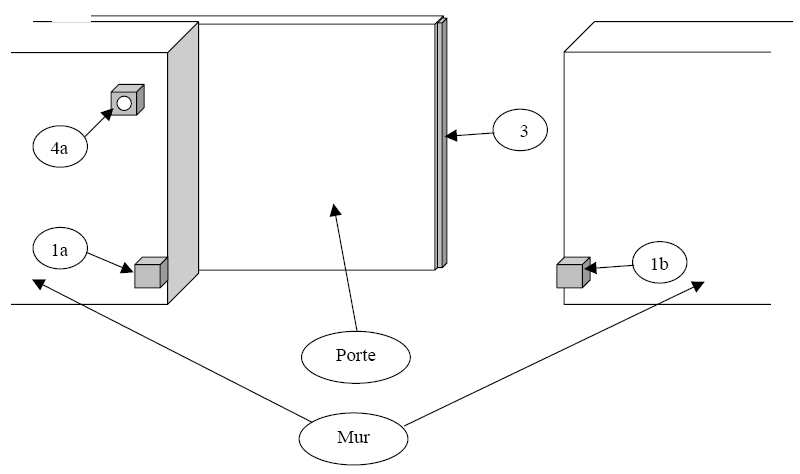
\includegraphics[width=2.25in,height=1.66667in]{14-Logique/Cours/pandoc/media/image180.png}Le thème du sujet est l'étude d'une porte automatique coulissant. Un usager peut déclencher l'ouverture de la porte depuis son véhicule par une action sur la télécommande qui lui a été fournie.

Le synoptique du portail est représenté ci-contre :

\emph{1a et 1b : barrière IR extérieure,}

\emph{2a et 2b : barrière IR intérieure,}

\emph{3 : palpeur,}

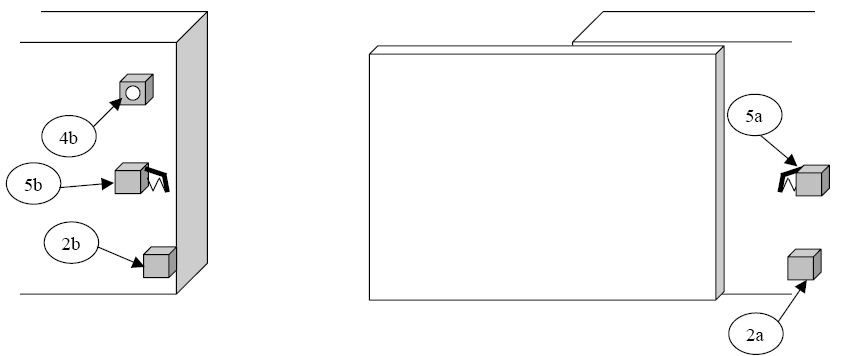
\includegraphics[width=2.54028in,height=1.48958in]{14-Logique/Cours/pandoc/media/image181.png}\emph{4a et 4b : capteurs de télécommande,}

\emph{5a et 5b : capteurs de fin de course}

Le moteur et l'armoire électrique de commande ne sont pas représentés.

Pour la sécurité des personnes, le système comporte deux barrières infra-rouges : l'une à l'intérieur du garage et l'autre à l'extérieur, ainsi qu'un palpeur qui est un capteur de contact localisé sur toute la tranche de la porte.

Les signaux logiques issus de ces dispositifs de sécurité sont notés I1, I2 et PP. Ils valent «~1~» lorsque le système est au repos et «~0 «~en cas d'activation de la sécurité.

L'activation d'une sécurité doit être sans effet sur le système si la porte est en train de s'ouvrir, par contre si la porte est en train de se refermer elle doit bien sûr se rouvrir.

Les variables logiques qui commandent la porte sont notées MO, MF et A pour « marche ouverture », « marche fermeture » et « arrêt ». Ces variables de commande sont liées à quatre variables de contrôle notées RX, FC, SO et SC qui sont décrites ci-dessous :

\begin{itemize}
\item
  RX vaut «~1~» si l'ordre d'ouverture est donné par une télécommande~;
\item
  SO vaut «~1~» si la porte est en train de s'ouvrir~;
\item
  FC vaut «~1~» si la porte touche un capteur de fin de course~;
\item
  SC vaut «~0~» si une sécurité est activée.
\end{itemize}

\begin{quote}
\begin{figure}
\centering
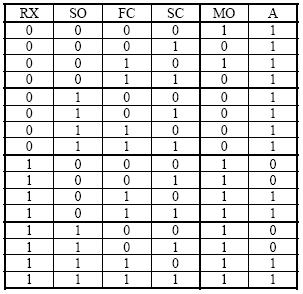
\includegraphics[width=2.20439in,height=2.146in]{14-Logique/Cours/pandoc/media/image182.jpeg}
\caption{table\_verite}
\end{figure}
\end{quote}

\begin{enumerate}
\def\labelenumi{\arabic{enumi}.}
\tightlist
\item
  \textbf{Travail demandé}
\end{enumerate}

\begin{enumerate}
\def\labelenumi{\arabic{enumi}.}
\item
  \textbf{Indiquer} pourquoi le palpeur est-il nécessaire en plus des deux barrières infra-rouges.
\item
  \textbf{Donner} l'expression de la variable SC en fonction de I1, I2 et PP.
\item
  A l'aide de la table de vérité donnée ci-dessus, \textbf{déterminer} l'expression la plus simple de A, à l'aide d'un tableau de Karnaugh.
\item
  \textbf{Représenter} sur le document réponse le schéma logique permettant d'obtenir A.
\item
  A l'aide de la table de vérité, \textbf{déterminer} l'expression la plus simple de MO, à l'aide d'un tableau de Karnaugh.
\item
  \textbf{Représenter,} sur le document réponse, le schéma logique permettant d'obtenir MO.
\end{enumerate}

\begin{figure}
\centering
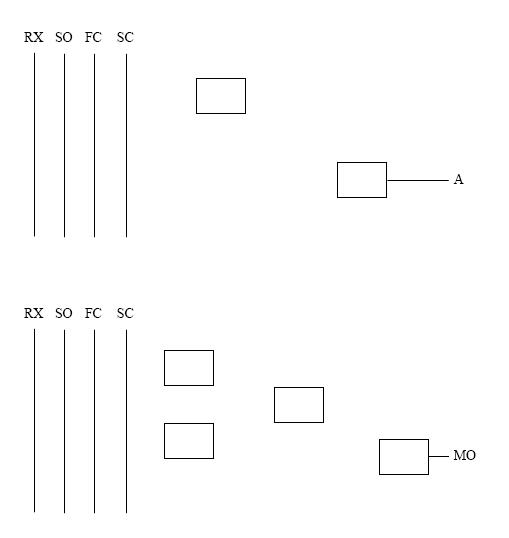
\includegraphics[width=6.66667in,height=7.03125in]{14-Logique/Cours/pandoc/media/image183.jpeg}
\caption{garage}
\end{figure}


\includegraphics[width=1.35556in,height=0.38889in]{14-Logique/Cours/pandoc/media/image178.png}\textbf{COMMANDE DE FEUX TRICOLORES}

Nous proposons de réaliser le décodeur d\textquotesingle un montage électronique permettant le fonctionnement des feux tricolores d\textquotesingle un carrefour routier comportant 2 voies (voie 1 et 2. voir le dessin du carrefour ci-contre).

Le principe du montage électronique complet est présenté dans le schéma synoptique ci-dessous :

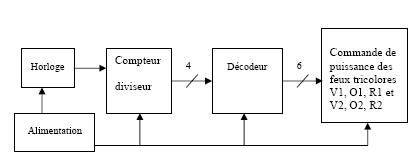
\includegraphics[width=4.16667in,height=1.89583in]{14-Logique/Cours/pandoc/media/image184.jpeg}\ul{Explication du principe :}

- L\textquotesingle horloge délivre une impulsion toutes les 2 secondes.

- Cette impulsion est appliquée à l'entrée d\textquotesingle horloge d\textquotesingle un compteur diviseur par 16.

- Les 4 sorties (a, b, c, d) du compteur délivrent des signaux logiques conformes aux chronogrammes qui suivent, et sont appliqués aux entrées du décodeur (voir chronogrammes).

\ul{Chronogrammes:}

\begin{figure}
\centering
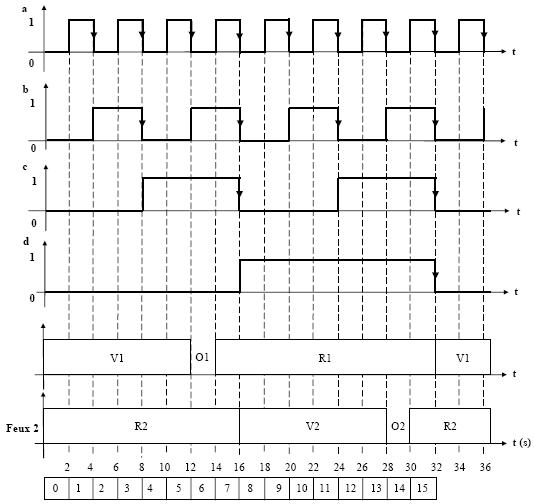
\includegraphics[width=5.38056in,height=5.07708in]{14-Logique/Cours/pandoc/media/image185.jpeg}
\caption{toto}
\end{figure}

~

\begin{enumerate}
\def\labelenumi{\arabic{enumi}.}
\item
  A partir des chronogrammes, donner la table de vérité de chaque sortie du décodeur en fonction des sorties du compteur.
\item
  En déduire les équations de chaque sortie.
\end{enumerate}


\includegraphics[width=1.35556in,height=0.38889in]{14-Logique/Cours/pandoc/media/image178.png}\textbf{PANNE D'UN HYDROPLANEUR}

\begin{longtable}[]{@{}
  >{\raggedright\arraybackslash}p{(\columnwidth - 4\tabcolsep) * \real{0.0541}}
  >{\raggedright\arraybackslash}p{(\columnwidth - 4\tabcolsep) * \real{0.5946}}
  >{\raggedright\arraybackslash}p{(\columnwidth - 4\tabcolsep) * \real{0.3378}}@{}}
\toprule\noalign{}
\begin{minipage}[b]{\linewidth}\raggedright
! {[}{]} ( 1 4 - L o g i q u e / C o u r s / p a n d o c / m e d i a / i m a g e 1 8 6 . p n g ) \{ w i d t h = '' 4 . 8 1 6 6 6 6 6 6 6 6 6 6 6 6 6 i n '' h e i g h t = '' 3 . 5 i n '' \}
\end{minipage} & \begin{minipage}[b]{\linewidth}\raggedright
\end{minipage} & \begin{minipage}[b]{\linewidth}\raggedright

\includegraphics{14-Logi que/Cours/pandoc/media /image187.jpeg}\{width= ``2.4833333333333334in'' height='' 1.7416666666666667in''\}
\end{minipage} \\
\midrule\noalign{}
\endhead
\bottomrule\noalign{}
\endlastfoot
\begin{minipage}[t]{\linewidth}\raggedright
D a n s l ' o b j e c t i f d ' o p t i m i s e r l e f o n c t i o n n e m e n t d ' u n h y d r o - p l a n e u r i l f a u t t e n i r c o m p t e d e t o u t e s l e s p r o c é d u r e s d e f o n c t i o n n e m e n t p r é v u e s , c o m m e c e l l e d ' a l e r t e e n c a s d e p a n n e d e l a t r a n s m i s s i o n d e s d o n n é e s , q u i i m p o s e d ' é m e t t r e u n s i g n a l d e d é t r e s s e p e r m e t t a n t d e v e n i r r e p ê c h e r l ' h y d r o - p l a n e u r .

À c h a q u e r e m o n t é e e n s u r f a c e , l ' h y d r o - p l a n e u r s e c o n n e c t e à u n r é s e a u s a n s f i l ( I R I D I U M ) a f i n d e t r a n s m e t t r e l e s d o n n é e s e n r e g i s t r é e s . L\\
' h y d r o - p l a n e u r d i s p o s e d e t r o i s a n t e n n e s l o g é e s d a n s l a d é r i v e e t d a n s c h a q u e a i l e r o n s t a b i l i s a t e u r . C e t t e s o l u t i o n i m p l i q u e q u e , p o u r é m e t t r e e n s u r f a c e , l ' e n g i n p i v o t e s u r l u i - m ê m e d ' u n q u a r t d e t o u r p o u r f a i r e é m e r g e r u n e d e s d e u x a n t e n n e s d é d i é e s a u r é s e a u I R I D I U M . P e n d a n t c e t t e p h a s e , l e d i s p o s i t i f d e b a s c u l e m e n t , q u i p e r m e t d e c o n t r ô l e r l e t a n g a g e d e l ' h y d r o - p l a n e u r , n ' e s t p a s a c t i f .

E n f i n d e c h a r g e d e s b a t t e r i e s o u e n c a s d e s o u c i t e c h n i q u e , l ' h y d r o - p l a n e u r d i s p o s e d ' u n e b a l i s e A R G O S ( d o n t l\\
' a n t e n n e e s t d a n s l a d é r i v e v e r t i c a l e ) q u i p e r m e t d e l e l o c a l i s e r e t d ' e n v o y e r u n n a v i r e p o u r l e r é c u p é r e r .\strut
\end{minipage} & \includegraphics[width=2.59167in,height=3.51667in]{14-Logique/Cours/pandoc/media/ image188.png} & \\
\end{longtable}

Dans ce cas de dysfonctionnement, l'hydro-planeur adopte le comportement décrit par le diagramme d'état ci-dessous :

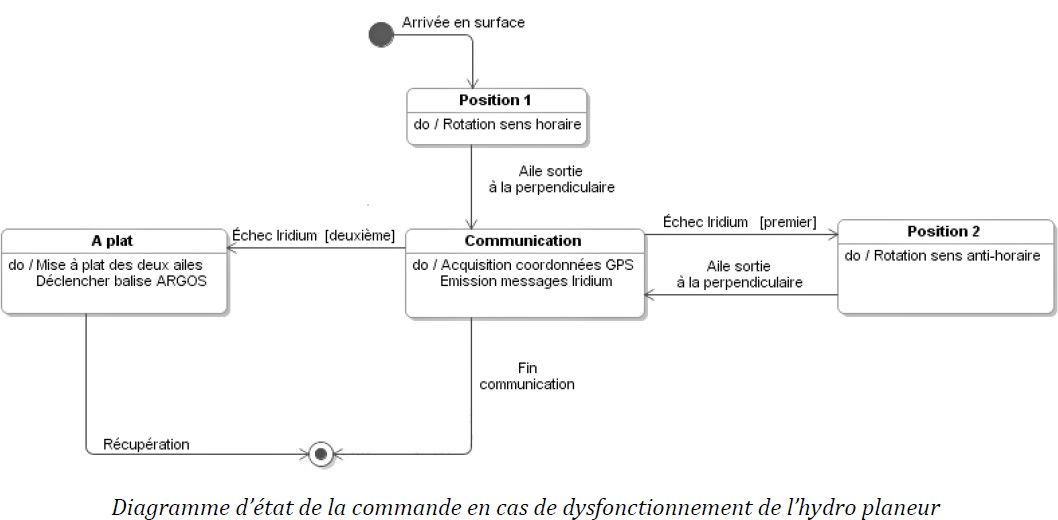
\includegraphics[width=6.57143in,height=3.62719in]{14-Logique/Cours/pandoc/media/image189.jpeg}

\begin{enumerate}
\def\labelenumi{\arabic{enumi}.}
\tightlist
\item
  Compléter les chronogrammes qui correspondent à la séquence des signaux de commande fournis par l'unité de traitement pour obtenir le fonctionnement souhaité dans le cas où la première et la deuxième transmission IRIDIUM échouent (lorsqu'un élément doit être activé, il sera représenté par un niveau haut).
\end{enumerate}

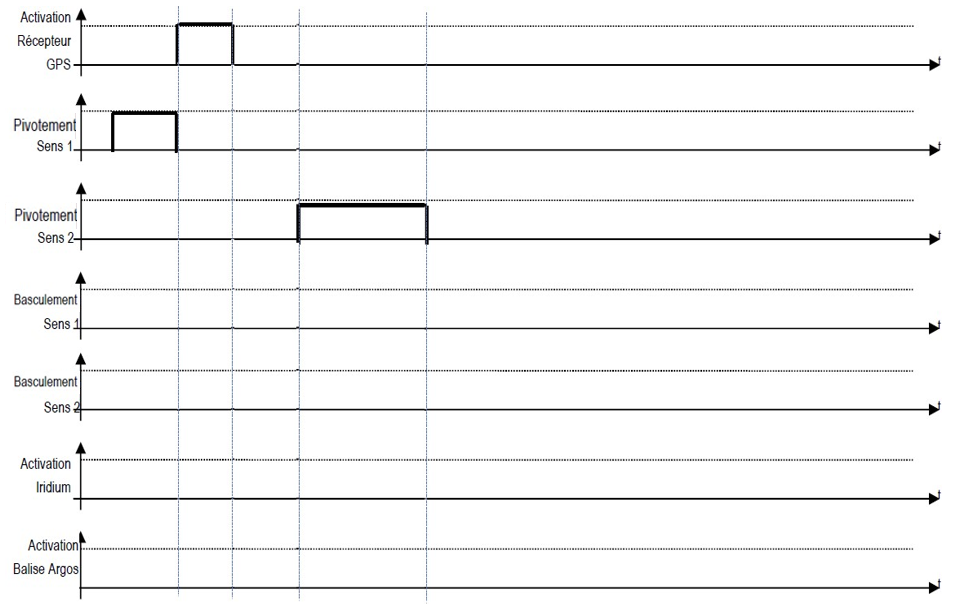
\includegraphics[width=7.26806in,height=2.00694in]{14-Logique/Cours/pandoc/media/image190.png}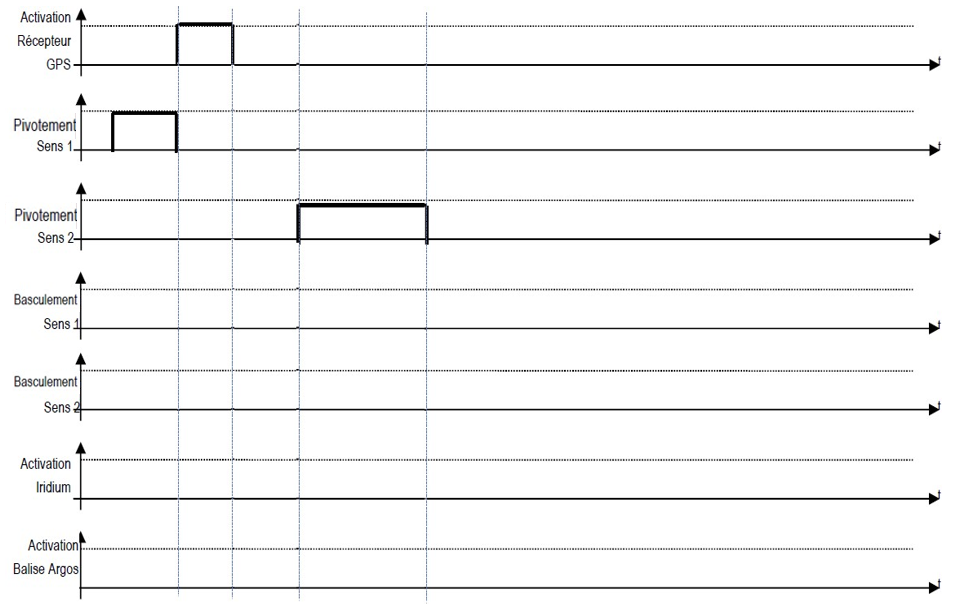
\includegraphics[width=7.26806in,height=1.29583in]{14-Logique/Cours/pandoc/media/image190.png}


\includegraphics[width=1.35556in,height=0.38889in]{14-Logique/Cours/pandoc/media/image178.png}\textbf{PORTE DE GARAGE BASCULANTE}

On souhaite qu\textquotesingle une porte de garage basculante ait le comportement suivant~:

\begin{itemize}
\item
  la mise en mouvement est réalisée par un moteur à 2 sens de rotation, permettant de l'ouvrir ou de la fermer~;
\item
  le moteur est alimenté par deux contacteurs, l'un pour l'ouverture (MO) et l'autre pour la fermeture (MF)~;
\item
  une fois la porte ouverte ou fermée, le moteur est à l\textquotesingle arrêt~;
\item
  en fin d\textquotesingle ouverture ou de fermeture, lorsque la porte arrive en butée, un capteur de courant à effet hall (CS) détecte une surintensité moteur~;
\item
  un boîtier mural comporte deux boutons, l\textquotesingle un pour la commande ouverture (BO), l\textquotesingle autre pour la fermeture (BF) ;
\item
  une télécommande possède un seul bouton (Tel). Si la porte est ouverte ou en phase d'ouverture, il commande la fermeture ; si elle est fermée ou en phase fermeture, il commande l\textquotesingle ouverture.
\item
  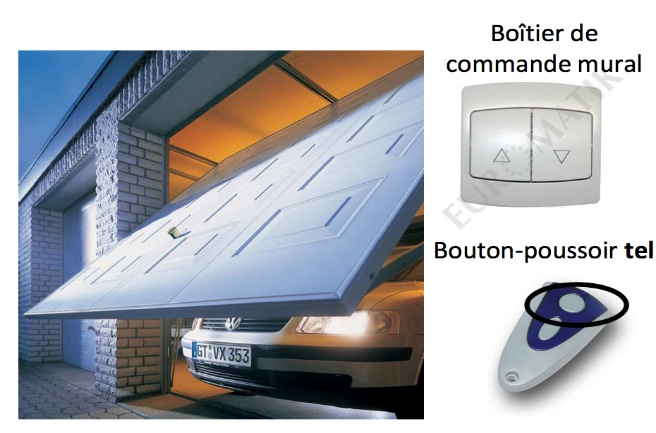
\includegraphics[width=2.98125in,height=1.97222in]{14-Logique/Cours/pandoc/media/image191.jpeg}les commandes d'ouverture ou de fermeture sont retenues uniquement si le bouton mural commandant le mouvement opposé n'est pas actionné~;
\item
  on suppose qu\textquotesingle à la mise en route, la porte est fermée.
\end{itemize}

Les consignes sont traitées comme des consignes impulsionnelles, sur front montant.

Nous n\textquotesingle étudierons pas les cas de mise en défaut~: coupure courant ou arrêt en position semi-ouverte.

\begin{enumerate}
\def\labelenumi{\arabic{enumi}.}
\item
  Lister et nommer les entrées (IHM et capteur) et sorties (IMH et préactionneur).
\item
  Lister les états possibles de la porte et les positionner dans un diagramme d'état.
\item
  Indiquer l\textquotesingle état initial et l\textquotesingle éventuel état final.
\item
  Compléter le diagramme avec l\textquotesingle ensemble des transitions possibles.
\item
  Compléter le diagramme avec l\textquotesingle ensemble des activités des différents états.
\item
  Compléter le chronogramme ci-dessous.
\end{enumerate}


\includegraphics[width=1.35556in,height=0.38889in]{14-Logique/Cours/pandoc/media/image178.png}~

\textbf{LAVE-LINGE ET REVEIL}

On souhaite modéliser le cycle complet d'un lave-linge comportant 5 étapes :

\begin{itemize}
\item
  Prélavage ;
\item
  Lavage ;
\item
  Rinçage ;
\item
  Essorage ;
\item
  Arrêt.
\end{itemize}

On définit les entrées/sorties suivantes :

\begin{itemize}
\item
  \textbf{M} : bouton poussoir « Marche » ;
\item
  \textbf{P} : « Prélavage » sélectionné ;
\item
  \textbf{C} : valeur courante (en minutes) d'un compteur permettant de mesurer la durée d'un état et qui est remis à zéro automatiquement au début de chaque état.
\end{itemize}

\begin{itemize}
\tightlist
\item
  Commande\_moteur : égale à 1 si le moteur doit tourner, sinon 0 ;
\end{itemize}

• Vitesse

\begin{enumerate}
\def\labelenumi{\Roman{enumi}.}
\tightlist
\item
  Les durées des différentes étapes de lavage sont fixées par le constructeur :
\end{enumerate}

\begin{itemize}
\item
  prélavage : 10 minutes avec le moteur qui tourne à 1000 tr/min;
\item
  lavage : 30 minutes avec le moteur qui tourne à 1000 tr/min ;
\item
  rinçage : 10 minutes avec le moteur qui tourne à 1000 tr/min;
\item
  essorage : 5 minutes avec le moteur qui tourne à 1400 tr/min.
\end{itemize}

\begin{enumerate}
\def\labelenumi{\arabic{enumi}.}
\item
  Recenser/définir les variables d'entrées et de sorties.
\item
  Recenser, nommer et tracer les états du système.
\item
  Tracer les transitions entre les états en fonction du comportement séquentiel souhaité ou observé.
\item
  Définir les conditions (et évènements) associées à chaque transition et les actions associées à chaque état.
\item
  Compléter ce graphe d'états afin de pouvoir interrompre le cycle du lave-linge quel que soit l'état actif de celui-ci. La variable d'entrée associée à la demande d'arrêt est la variable binaire Stop.

  \begin{enumerate}
  \def\labelenumii{\arabic{enumii}.}
  \tightlist
  \item
    \textbf{Réveil}
  \end{enumerate}
\end{enumerate}

Considérons un réveil simplifié :

\begin{itemize}
\item
  On peut mettre l'alarme `\emph{on}' ou `\emph{off}' ;
\item
  Quand l'heure courante devient égale à l'heure d'alarme, le réveil \textgreater{} sonne sans s'arrêter.
\item
  On peut interrompre la sonnerie.
\end{itemize}

\begin{enumerate}
\def\labelenumi{\arabic{enumi}.}
\item
  Dessiner le diagramme d'états correspondant.
\item
  Compléter le diagramme d'états précédent pour prendre en compte le fait que la sonnerie du réveil s'arrête d'elle-même au bout d'un certain temps.
\end{enumerate}


\includegraphics[width=1.35556in,height=0.38889in]{14-Logique/Cours/pandoc/media/image178.png}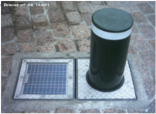
\includegraphics[width=0.70486in,height=0.51636in]{14-Logique/Cours/pandoc/media/image192.png}\textbf{BORNE SOLAIRE}

\emph{(\ul{Source} : ATS 2010)}

\begin{enumerate}
\def\labelenumi{\arabic{enumi}.}
\tightlist
\item
  \textbf{Mise en situation}
\end{enumerate}

\begin{quote}
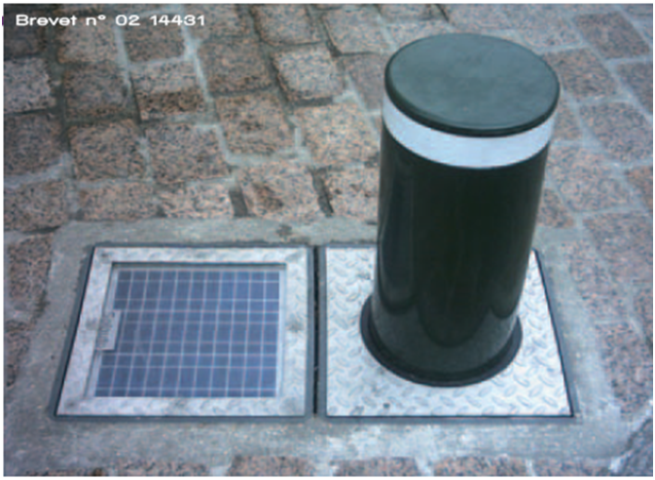
\includegraphics[width=3.15069in,height=2.18403in]{14-Logique/Cours/pandoc/media/image193.png}Le dispositif étudié est un système permettant de limiter ou d\textquotesingle interdire la circulation dans des zones à accès réservé. Ce dispositif comporte :
\end{quote}

\begin{itemize}
\item
  un caisson intégrant la partie opérative, à savoir une borne \textgreater{} motorisée rétractable dans le sol,
\item
  un caisson intégrant la partie commande comportant :
\end{itemize}

\begin{quote}
- une platine électronique de gestion,

- une batterie d\textquotesingle alimentation électrique du système,

- des cellules photovoltaïques assurant la charge de la batterie.

Selon son concept innovant et breveté, le système utilise un module solaire pour recharger sa batterie. L\textquotesingle installation d\textquotesingle une borne de ce type ne nécessite aucune tranchée, aucun raccordement, ni abonnement EDF ; son alimentation est gratuite et peut être envisagée sur n\textquotesingle importe quel site.

Cependant, le fonctionnement du système est limité à un nombre de cycles dont la valeur dépend des conditions d\textquotesingle ensoleillement. La problématique majeure pour ce système est donc d\textquotesingle atteindre une autonomie suffisante, tout en minimisant le coût et l\textquotesingle encombrement des moyens de production et de stockage de l\textquotesingle énergie électrique. Le panneau, la batterie et la motorisation du système sont reliés grâce à un dispositif appelé régulateur de charge, qui est étudier ici.
\end{quote}

\textbf{\emph{Régulateur de charge pour système photovoltaïque}} (Extraits documentation constructeur)

\ul{A. Présentation générale}

Le régulateur de charge est un dispositif électronique au fonctionnement entièrement automatique. Il relie le panneau photovoltaïque, la batterie et les équipements destinataires de l'électricité produite.

Sa fonction principale est de contrôler l'état de charge de la batterie. Il autorise la charge complète de celle-ci en éliminant le risque de surcharge. Il peut également interrompre l'alimentation des destinataires pour éviter une décharge profonde. Le régulateur, décrit ci-dessous, mesure la tension aux bornes de la batterie et assure une régulation série « tout ou rien ».

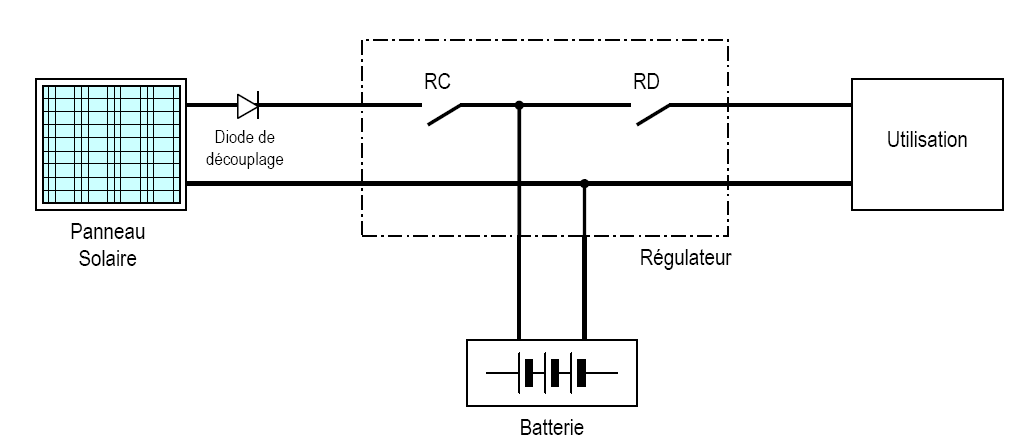
\includegraphics[width=4.58681in,height=1.8875in]{14-Logique/Cours/pandoc/media/image195.png}\ul{B. Schéma de principe}

\ul{C. Principe de fonctionnement}

- Fonctionnement normal : les contacts des relais RC et RD sont fermés.

- Limitation de charge : Si la tension batterie dépasse la valeur EB{[}max{]}, le relais RC s'ouvre. Il se referme automatiquement au bout de 10 minutes, sauf si la tension batterie est devenue inférieure à EB{[}min{]} pendant cette durée.

- Limitation de décharge : Si la tension batterie devient inférieure à la valeur EB{[}min{]}, le relais RD s'ouvre. Il se referme lorsque la tension a atteint la valeur EB{[}nominal{]}.

\begin{enumerate}
\def\labelenumi{\arabic{enumi}.}
\tightlist
\item
  \textbf{Étude du fonctionnement du régulateur de charge}
\end{enumerate}

\begin{enumerate}
\def\labelenumi{\arabic{enumi}.}
\item
  Compléter le \textbf{document réponse}, en indiquant l'état des contacts RC et RD (état logique « 0 » pour ouvert), selon l'état de charge de la batterie.
\item
  Toujours sur le \textbf{document réponse}, indiquer le sens des transferts d'énergie en précisant pour chaque élément, s'il reçoit de l'énergie (R), s'il fournit de l'énergie (F), ou s'il n'est pas en service (∅).
\item
  Représenter le fonctionnement en utilisant le formalisme des graphes d'états.

  \begin{enumerate}
  \def\labelenumii{\arabic{enumii}.}
  \tightlist
  \item
    \textbf{Document Réponse}
  \end{enumerate}
\end{enumerate}

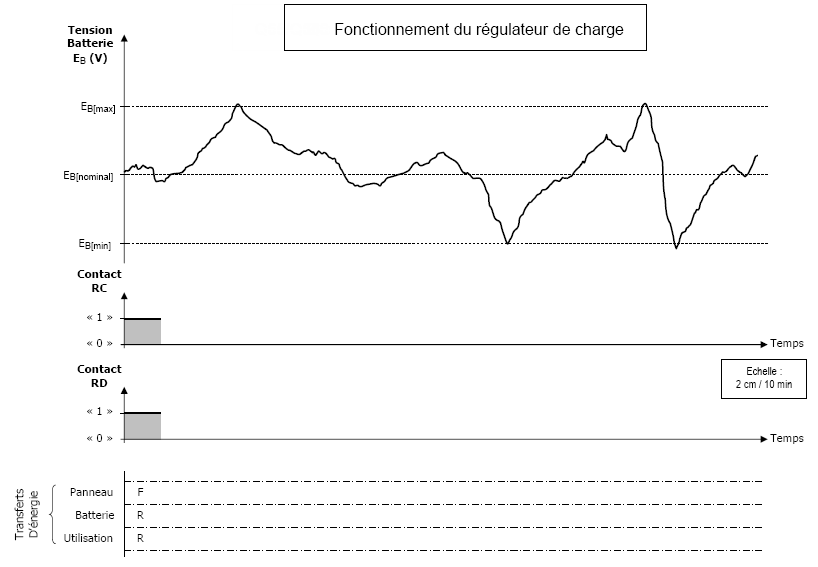
\includegraphics[width=7.28225in,height=5.04709in]{14-Logique/Cours/pandoc/media/image196.png}


\includegraphics[width=1.35556in,height=0.38889in]{14-Logique/Cours/pandoc/media/image178.png}\textbf{ROBOT MARTIEN SPIRIT}

\begin{figure}
\centering
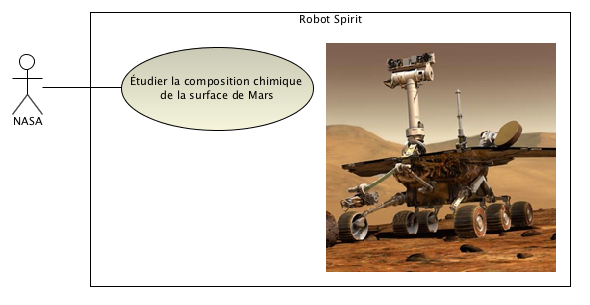
\includegraphics[width=3.57014in,height=1.84524in]{14-Logique/Cours/pandoc/media/image197.png}
\caption{Macintosh HD:Users:olivierlegallo:Documents:Dossiers du bureau:Lycée:TD, colles, devoirs:2014-15:PSI*:Devoirs:DS6:Spirit:UC Spirit.tiff}
\end{figure}

\begin{figure}
\centering
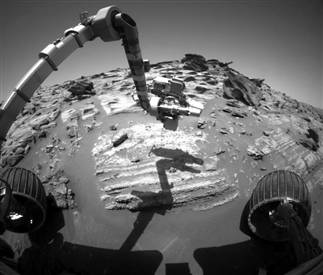
\includegraphics[width=2.03403in,height=1.73125in]{14-Logique/Cours/pandoc/media/image198.jpeg}
\caption{Macintosh HD:Users:olivierlegallo:Desktop:Mars\_Spirit\_Home\_Plate.jpg}
\end{figure}

Le robot SPIRIT a été conçu par la NASA pour étudier la composition chimique de la surface de la planète Mars. Les principaux composants de ce robot sont~:

\begin{itemize}
\item
  Un corps, appelé «~Warm Electronic Box~», dont la fonction est \textgreater{} d'assurer la liaison entre les divers composants. Il supporte les \textgreater{} batteries qui sont chargées par des capteurs solaires. Il protège \textgreater{} également l'électronique embarquée des agressions extérieures.
\item
  Une tête périscopique orientable dont la fonction est d'orienter le \textgreater{} système de vision appelé «~Pancam~» (Panoramic Camera) qui se \textgreater{} trouve à 1,40 m de hauteur. Ce dernier fournit une vue en trois \textgreater{} dimensions de l'environnement. Le traitement des images acquises \textgreater{} par les caméras du Pancam permet à Spirit de réaliser une \textgreater{} cartographie des terrains et donc de trouver de manière autonome \textgreater{} son chemin en évitant les obstacles. Cette autonomie de \textgreater{} déplacement est renforcée par l'utilisation de quatre caméras de \textgreater{} direction situées sur le corps.
\item
  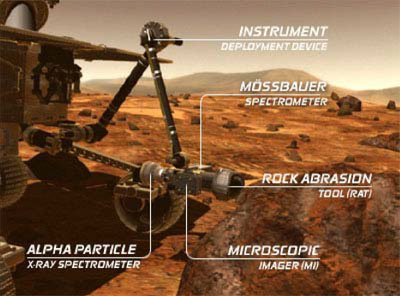
\includegraphics{14-Logique/Cours/pandoc/media/image199.jpeg}\{width=``3.9743055555555555in'' \textgreater{} height=``2.939583333333333in''\}Un bras articulé (image ci-contre), \textgreater{} dont la fonction est d'amener un barillet portant quatre outils \textgreater{} (une foreuse, un microscope et deux spectromètres) à proximité \textgreater{} d'une roche à étudier. L'étude de la roche par ces quatre outils \textgreater{} se fait par des carottages horizontaux.
\item
  Six roues, animées chacune par un motoréducteur, dont la fonction \textgreater{} est d'assurer le déplacement de Spirit sur un sol caillouteux. Les \textgreater{} deux roues avant et arrière possèdent de plus un moteur de \textgreater{} direction permettant au robot d'effectuer des changements de \textgreater{} direction jusqu'à un demi-tour sur place.
\item
  Un système de communication et des antennes haute et basse \textgreater{} fréquence, dont la fonction est de permettre à Spirit de \textgreater{} communiquer avec la terre.
\end{itemize}

Le BDD qui suit précise cette structure matérielle.

\begin{figure}
\centering
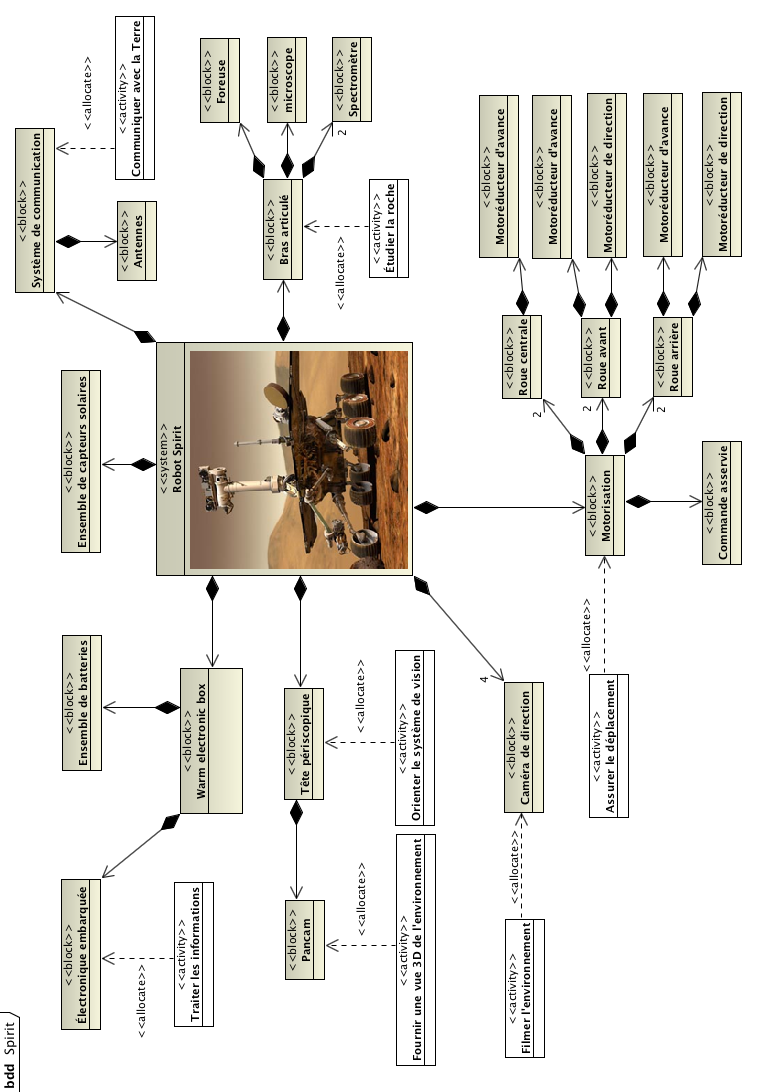
\includegraphics[width=6.96875in,height=9.96111in]{14-Logique/Cours/pandoc/media/image200.png}
\caption{Macintosh HD:Users:olivierlegallo:Documents:Dossiers du bureau:Lycée:TD, colles, devoirs:2014-15:PSI*:Devoirs:DS6:Spirit:BDD Spirit.tiff}
\end{figure}

On s'intéresse ici uniquement à la phase de prospection. Comme précisé précédemment, l'analyse est réalisée grâce à quatre outils installés sur un barillet rotatif~:

\begin{itemize}
\item
  La foreuse à lame (notée fo)~: elle est utilisée pour obtenir une \textgreater{} surface analysable. Afin de supprimer la croûte rocheuse, un trou \textgreater{} cylindrique de profondeur minimale est effectué. Un capteur mesure \textgreater{} la profondeur de perçage et envoie l'information pt (perçage \textgreater{} terminé) lorsque l'objectif est atteint. Le perçage normal se fait \textgreater{} à vitesse minimale et effort maximal. L'information fo\_r signale \textgreater{} que la foreuse est rentrée en position de repos, l'information \textgreater{} fo\_s signale que la foreuse est sortie, prête à l'emploi.
\item
  Le microscope optique (noté mi)~: il renseigne sur la morphologie de \textgreater{} la roche (taille des particules, agencement, texture, etc.). \textgreater{} L'électronique signale la fin de l'analyse optique par \textgreater{} l'information fin\_a. L'information mi\_r signale que le microscope \textgreater{} est rentré en position repos, l'information mi\_s que le microscope \textgreater{} est sorti, prêt à l'emploi.
\item
  L'analyseur APSX (noté ap)~: il mène des analyses aux rayons X et α, \textgreater{} de manière à déterminer la composition élémentaire de la roche.
\item
  Le spectromètre de Moessbauer (noté sp)~: il permet de détecter la \textgreater{} présence de minéraux ferreux et de quantifier la teneur en Fe\textsuperscript{2+} \textgreater{} et Fe\textsuperscript{3+}.
\end{itemize}

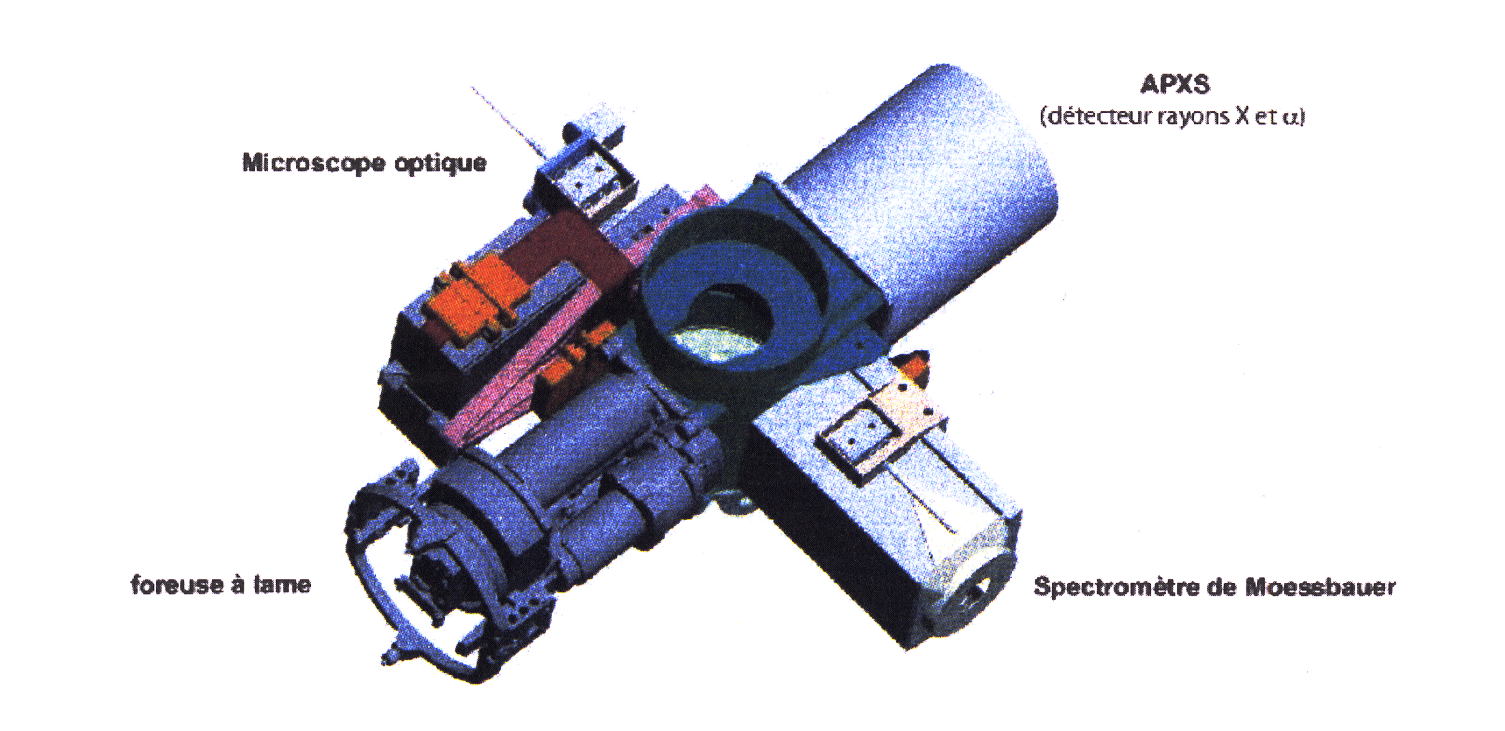
\includegraphics[width=6.84514in,height=3.32569in]{14-Logique/Cours/pandoc/media/image201.png}

Figure 8~: Détail du barillet d'exploration

Initialement, la foreuse se trouve face à la surface à étudier (la position du barillet est mesurée par un capteur angulaire). Le déroulement normal d'une phase de prospection est spécifié par le diagramme d'états page suivante.

La phase de prospection débute lorsque la commande de départ d est donnée et que le barillet se trouve foreuse face à la surface (information p0 délivrée par le capteur angulaire).

Le perçage s'effectue alors (à vitesse minimale et effort maximal) jusqu'à ce que la profondeur voulue soit atteinte (information pt), puis la foreuse se rétracte et le barillet tourne de 90° (position p90) dans le sens positif.

Puis viennent les phases d'analyse optique, APSX et spectromètre avec une rotation de 90° du barillet à chaque fois, jusqu'au retour à la position initiale du barillet.

Les phases d'analyse ASPX et spectromètre ne sont pas étudiées et donc les états composites correspondants ne sont pas fournis.

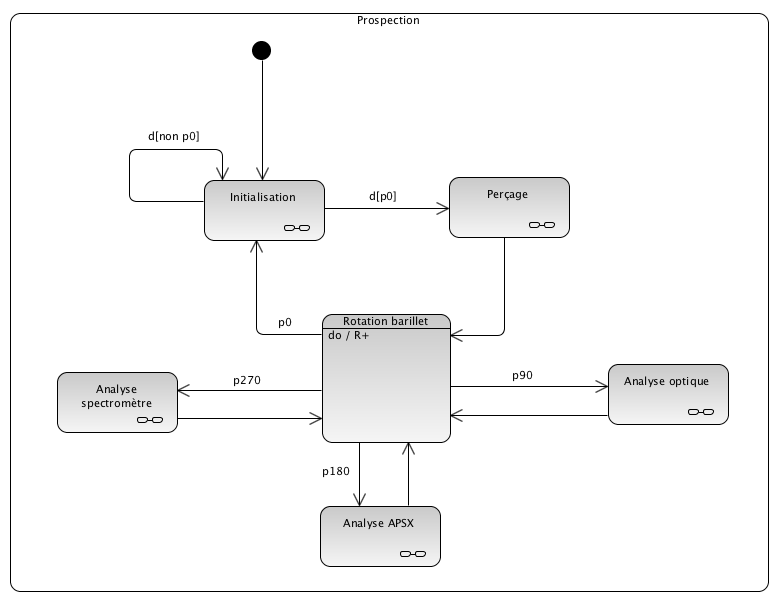
\includegraphics[width=6.18264in,height=4.75764in]{14-Logique/Cours/pandoc/media/image202.png}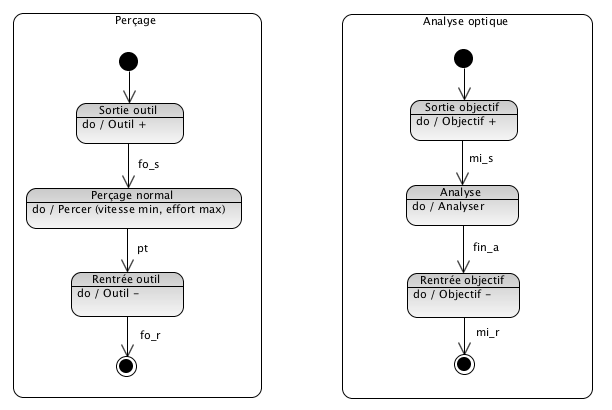
\includegraphics[width=4.84444in,height=3.24583in]{14-Logique/Cours/pandoc/media/image203.png}

En pratique, ce fonctionnement normal peut être perturbé par deux situations~:

\begin{itemize}
\item
  \textbf{Pathologie 1- échec de la phase de perçage~:} le forage peut \textgreater{} échouer si la roche se révèle trop résistante. Dans ce cas, on \textgreater{} renonce à l'analyse et le système doit revenir en situation \textgreater{} initiale.
\item
  \textbf{Pathologie 2 - échec de la phase d'analyse~:} le microscope \textgreater{} optique de haute précision a une profondeur de champ très réduite, \textgreater{} en conséquence, si l'état de surface à l'issue de la phase de \textgreater{} perçage est médiocre, l'analyse optique ne peut pas être menée. Il \textgreater{} est alors nécessaire de recommencer la phase de perçage, cette \textgreater{} fois à vitesse maximale et effort minimal, ces conditions \textgreater{} permettant d'améliorer notablement l'état d'une surface \textgreater{} préexistante.
\end{itemize}

\textbf{Questions}

Les réponses sont à apporter sur le document-réponses fourni page suivante.

\textbf{Question 1~:}

Proposer une modification de l'état composite de perçage permettant de~:

- renoncer au perçage si la profondeur attendue n'est pas atteinte au delà d'une durée maximale t\_max~;

- créer une variable «~perçage échoué~» telle que~:

perçage échoué = 0 si le perçage est réussi

perçage échoué = 1 en cas d'échec.

\textbf{Question 2~:}

Modifier le diagramme de prospection en conséquence pour que, dans le cas d'un échec du perçage, le système revienne en situation initiale.

\textbf{Question 3~:}

En fonctionnement normal, l'électronique signale la fin de l'analyse optique par l'information fin\_a. Dans le cas de la pathologie 2, cette information n'est jamais validée mais le système valide une information S\_imp (surface impropre). Proposer une modification de l'état composite d'analyse optique permettant de~:

- renoncer à l'analyse optique si l'information S\_imp est reçue~;

- créer une variable «~analyse échouée~» telle que~:

analyse échouée = 0 si l'analyse est réussie

analyse échouée = 1 en cas d'échec.

\textbf{Question 4~:}

Poursuivre la modification du diagramme de prospection pour que, dans le cas d'un échec de l'analyse optique, la phase de perçage soit relancée.

\textbf{Question 5~:}

Modifier pour finir l'état composite de perçage de manière à ce que les conditions de forage correspondent à la façon dont cet état a été activé~: perçage normal (vitesse min, effort max) ou perçage fin (vitesse max, effort min) s'il s'agit d'améliorer la surface.

\begin{figure}
\centering
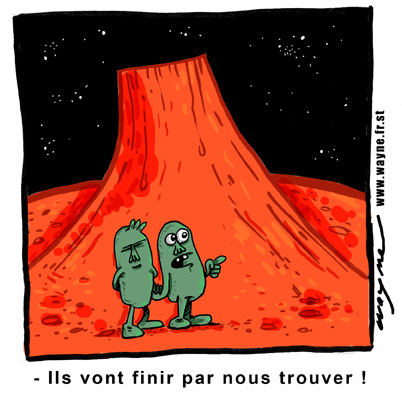
\includegraphics[width=1.83611in,height=1.94931in]{14-Logique/Cours/pandoc/media/image204.jpeg}
\caption{Mars}
\end{figure}

\textbf{DOCUMENT-RÉPONSES}

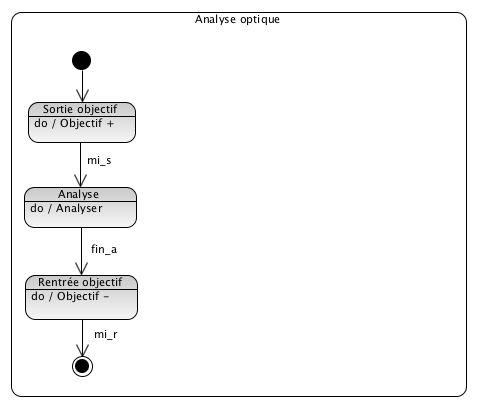
\includegraphics[width=3.6in,height=3.15486in]{14-Logique/Cours/pandoc/media/image205.png}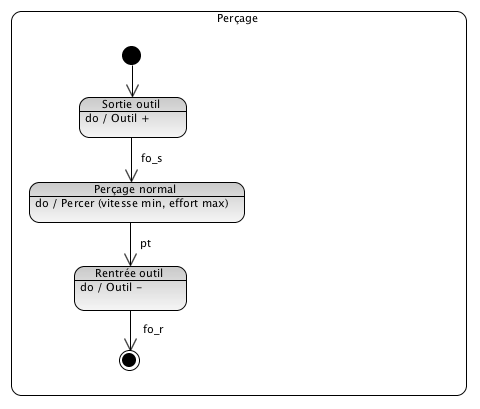
\includegraphics[width=3.57708in,height=3.12431in]{14-Logique/Cours/pandoc/media/image206.png}

\textbf{Q1 Q3}

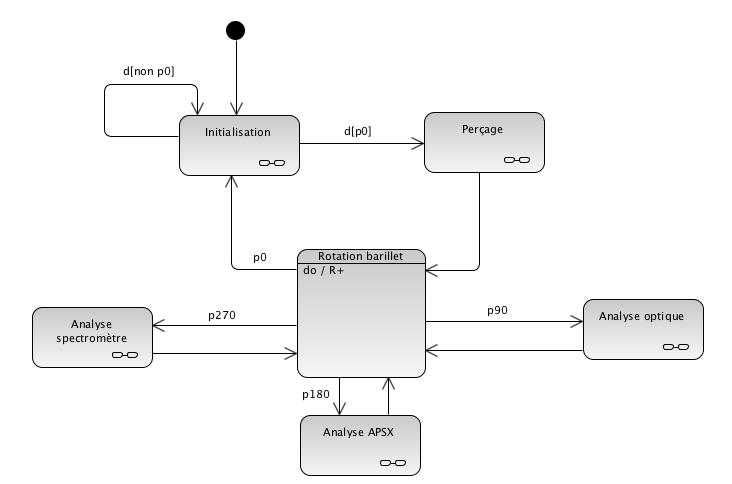
\includegraphics[width=5.59167in,height=3.55208in]{14-Logique/Cours/pandoc/media/image207.png}\textbf{Q2 et Q4}

\begin{figure}
\centering
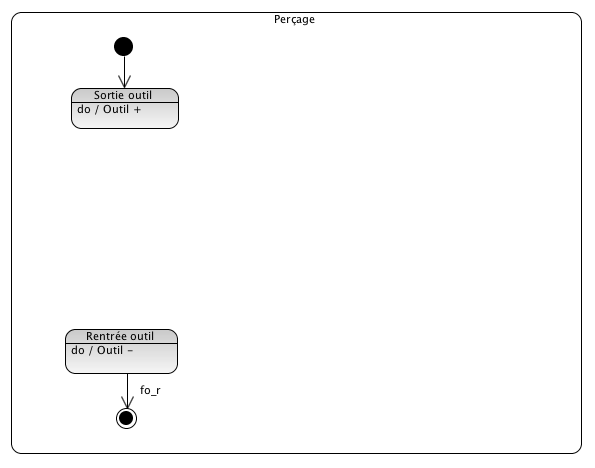
\includegraphics[width=4.54514in,height=3.42639in]{14-Logique/Cours/pandoc/media/image208.png}
\caption{Macintosh HD:Users:olivierlegallo:Desktop:Sans titre.tiff}
\end{figure}

\textbf{Q5}

\textbf{CORRECTION}

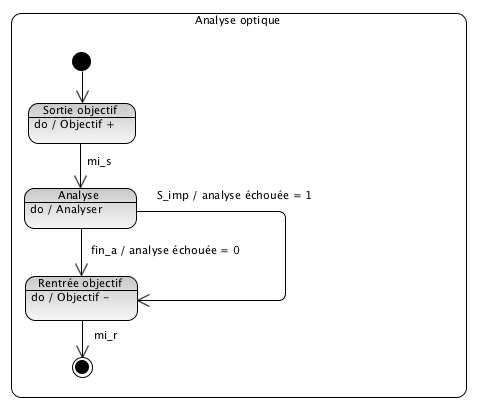
\includegraphics[width=3.63125in,height=3.13958in]{14-Logique/Cours/pandoc/media/image209.png}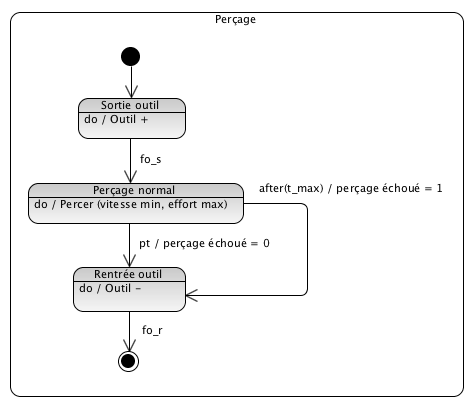
\includegraphics[width=3.54861in,height=3.10903in]{14-Logique/Cours/pandoc/media/image210.png}

\textbf{Q1 Q3}

\begin{figure}
\centering
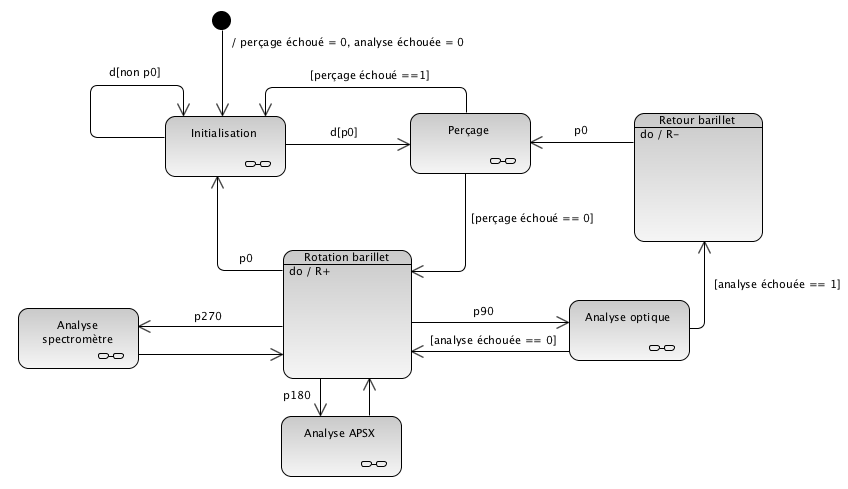
\includegraphics[width=6.47778in,height=3.73542in]{14-Logique/Cours/pandoc/media/image211.png}
\caption{Macintosh HD:Users:olivierlegallo:Desktop:Sans titre.tiff}
\end{figure}

\textbf{Q2 et Q4}

\begin{figure}
\centering
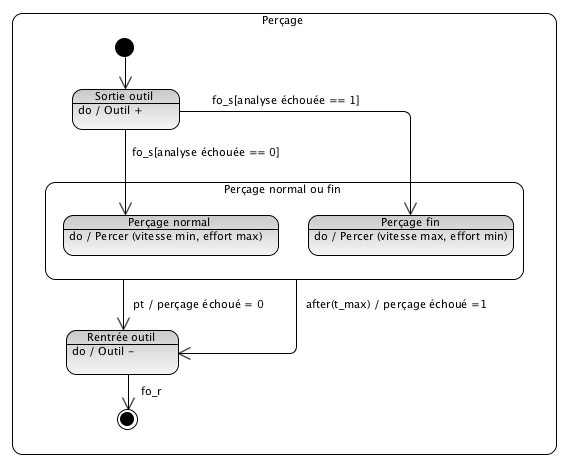
\includegraphics[width=4.36181in,height=3.40486in]{14-Logique/Cours/pandoc/media/image212.png}
\caption{Macintosh HD:Users:olivierlegallo:Desktop:Sans titre.tiff}
\end{figure}

\textbf{Q5}


\includegraphics[width=1.35556in,height=0.38889in]{14-Logique/Cours/pandoc/media/image178.png}\textbf{Gus : Une révolution dans le déplacement}


\includegraphics[width=1.125in,height=2.05833in]{14-Logique/Cours/pandoc/media/image213.emf}Depuis plus de six ans la société OPUS TECHNOLOGIES conçoit, met au point et fabrique un fauteuil électrique particulièrement innovant, appelé GUS, acronyme de \textbf{G}yropode \textbf{U}tilitaire et \textbf{S}portif (figures 1 et 2).

Ce fauteuil est destiné, aussi bien aux Personnes à Mobilité Réduite (PMR), qu'aux séniors à la recherche d'une assistance dans les déplacements du quotidien.

Son design, son principe de fonctionnement basé sur une solution de type Gyropode et sa maniabilité sont pensés pour modifier le regard de chacun sur les handicapés en fauteuil roulant et plus généralement le regard que nous portons sur le handicap (figure 2).

Le diagramme de contexte de la figure 3, présente ainsi le GUS dans son environnement immédiat.


\includegraphics[width=5.59167in,height=5.075in]{14-Logique/Cours/pandoc/media/image214.emf}

\textbf{\emph{Diagrammes états transitions du fonctionnement du GUS}}

Le fonctionnement du GUS commence lors de l'installation de la personne sur le fauteuil. Cette action déclenche l'événement \textbf{ON}.

Il se termine lorsque la personne quitte le fauteuil. Cette action déclenche l'événement OFF.

En situation de fonctionnement, on distingue deux modes principaux. Ils correspondent à des états dans lequel le GUS peut se trouver.

\begin{itemize}
\item
  Un mode \textbf{Arrêt} dans lequel le béquillage est actif et durant lequel les asservissements sont désactivés. Ce mode ne consomme quasiment pas d'énergie car seule la veille de la carte de commande est activée.
\item
  Un mode \textbf{Marche} dans lequel le béquillage est inactif et durant lequel les asservissements sont actifs. Ce mode correspond au fonctionnement normal du fauteuil et autorise tous les déplacements en assurant l'équilibre du fauteuil. Lors de ce mode, les paramètres du GUS sont surveillés en temps réel. Le système de béquillage se met en fonctionnement, désactivant les asservissements, si au moins un des paramètres indique qu'un risque de perte d'équilibre est détecté. GUS passe alors en mode \textbf{Arrêt}.
\end{itemize}

Les événements à prendre en considération sont :

\begin{itemize}
\item
  ON : Début d'utilisation du fauteuil lors de l'installation de la personne ;
\item
  OFF : Fin d'utilisation du fauteuil et retrait de la personne.
\end{itemize}

\begin{itemize}
\item
  CMB : Commande Manuelle de Béquillage (béquillage actif) ;
\item
  CMD : Commande Manuelle de Dé-béquillage (béquillage inactif) ;
\item
  CAB : Commande Automatique de Béquillage (béquillage actif)
\end{itemize}

\textbf{Question 1 :} A l'aide des informations précédentes, compléter le document réponse DR1, correspondant au modèle de comportement macroscopique régissant le fonctionnement du GUS.


\includegraphics[width=4.56667in,height=3.19042in]{14-Logique/Cours/pandoc/media/image215.emf}

En réalité, lors de l'activation du mode Marche, deux sous-ensembles sont activés en même temps, chacun d'entre eux ayant une fonction bien précise. Le premier de nom \textbf{Déplacement/Asservissement} gère l'équilibre du fauteuil et son déplacement suivant les souhaits de la personne. Le second nommé \textbf{Surveillance} veille au respect des paramètres critiques du GUS et déclenche l'évènement \textbf{CAB} si nécessaire, évitant ainsi toute chute accidentelle.

\textbf{Question 2 :} A l'aide de la description de l'état \textbf{Marche}, compléter le document réponse DR2, correspondant au modèle de comportement complet régissant le fonctionnement du GUS.


\includegraphics[width=6.3in,height=4.56389in]{14-Logique/Cours/pandoc/media/image216.emf}

\textbf{Question 3 :} Vis-à-vis de la modélisation comportementale abordée et sachant que l'opération de béquillage se fait en moins de 200 ms, conclure sur le respect des exigences 1.2 et 1.2.1 du document technique DT1.


\includegraphics[width=6.3in,height=9.75in]{14-Logique/Cours/pandoc/media/image217.emf}

\begin{center}\rule{0.5\linewidth}{0.5pt}\end{center}

\hypertarget{inventaire-des-images}{%
\subsection{Inventaire des images}\label{inventaire-des-images}}

14-Logique/Cours/pandoc/media/image1.png 14-Logique/Cours/pandoc/media/image10.png 14-Logique/Cours/pandoc/media/image100.png 14-Logique/Cours/pandoc/media/image101.png 14-Logique/Cours/pandoc/media/image102.emf 14-Logique/Cours/pandoc/media/image103.png 14-Logique/Cours/pandoc/media/image104.png 14-Logique/Cours/pandoc/media/image105.png 14-Logique/Cours/pandoc/media/image106.png 14-Logique/Cours/pandoc/media/image107.png 14-Logique/Cours/pandoc/media/image108.png 14-Logique/Cours/pandoc/media/image109.png 14-Logique/Cours/pandoc/media/image11.jpeg 14-Logique/Cours/pandoc/media/image111.png 14-Logique/Cours/pandoc/media/image112.jpeg 14-Logique/Cours/pandoc/media/image113.png 14-Logique/Cours/pandoc/media/image114.png 14-Logique/Cours/pandoc/media/image115.png 14-Logique/Cours/pandoc/media/image118.png 14-Logique/Cours/pandoc/media/image119.png 14-Logique/Cours/pandoc/media/image12.jpeg 14-Logique/Cours/pandoc/media/image120.png 14-Logique/Cours/pandoc/media/image121.png 14-Logique/Cours/pandoc/media/image122.emf 14-Logique/Cours/pandoc/media/image123.png 14-Logique/Cours/pandoc/media/image124.png 14-Logique/Cours/pandoc/media/image125.png 14-Logique/Cours/pandoc/media/image126.png 14-Logique/Cours/pandoc/media/image127.png 14-Logique/Cours/pandoc/media/image128.png 14-Logique/Cours/pandoc/media/image129.png 14-Logique/Cours/pandoc/media/image13.jpeg 14-Logique/Cours/pandoc/media/image130.emf 14-Logique/Cours/pandoc/media/image131.emf 14-Logique/Cours/pandoc/media/image132.emf 14-Logique/Cours/pandoc/media/image133.emf 14-Logique/Cours/pandoc/media/image134.emf 14-Logique/Cours/pandoc/media/image135.emf 14-Logique/Cours/pandoc/media/image136.emf 14-Logique/Cours/pandoc/media/image137.jpeg 14-Logique/Cours/pandoc/media/image138.jpeg 14-Logique/Cours/pandoc/media/image139.jpeg 14-Logique/Cours/pandoc/media/image14.png 14-Logique/Cours/pandoc/media/image140.jpeg 14-Logique/Cours/pandoc/media/image141.emf 14-Logique/Cours/pandoc/media/image142.emf 14-Logique/Cours/pandoc/media/image143.emf 14-Logique/Cours/pandoc/media/image144.jpeg 14-Logique/Cours/pandoc/media/image145.png 14-Logique/Cours/pandoc/media/image146.png 14-Logique/Cours/pandoc/media/image147.png 14-Logique/Cours/pandoc/media/image148.png 14-Logique/Cours/pandoc/media/image149.emf 14-Logique/Cours/pandoc/media/image15.wmf 14-Logique/Cours/pandoc/media/image150.jpeg 14-Logique/Cours/pandoc/media/image151.png 14-Logique/Cours/pandoc/media/image152.jpeg 14-Logique/Cours/pandoc/media/image153.png 14-Logique/Cours/pandoc/media/image154.jpeg 14-Logique/Cours/pandoc/media/image155.png 14-Logique/Cours/pandoc/media/image156.png 14-Logique/Cours/pandoc/media/image157.png 14-Logique/Cours/pandoc/media/image158.png 14-Logique/Cours/pandoc/media/image159.png 14-Logique/Cours/pandoc/media/image16.wmf 14-Logique/Cours/pandoc/media/image160.jpeg 14-Logique/Cours/pandoc/media/image161.jpeg 14-Logique/Cours/pandoc/media/image162.jpeg 14-Logique/Cours/pandoc/media/image163.png 14-Logique/Cours/pandoc/media/image164.jpeg 14-Logique/Cours/pandoc/media/image165.jpeg 14-Logique/Cours/pandoc/media/image167.jpeg 14-Logique/Cours/pandoc/media/image168.png 14-Logique/Cours/pandoc/media/image169.png 14-Logique/Cours/pandoc/media/image17.wmf 14-Logique/Cours/pandoc/media/image170.jpeg 14-Logique/Cours/pandoc/media/image171.jpeg 14-Logique/Cours/pandoc/media/image172.png 14-Logique/Cours/pandoc/media/image173.jpeg 14-Logique/Cours/pandoc/media/image174.jpeg 14-Logique/Cours/pandoc/media/image175.png 14-Logique/Cours/pandoc/media/image176.png 14-Logique/Cours/pandoc/media/image177.png 14-Logique/Cours/pandoc/media/image178.png 14-Logique/Cours/pandoc/media/image18.wmf 14-Logique/Cours/pandoc/media/image180.png 14-Logique/Cours/pandoc/media/image181.png 14-Logique/Cours/pandoc/media/image182.jpeg 14-Logique/Cours/pandoc/media/image183.jpeg 14-Logique/Cours/pandoc/media/image184.jpeg 14-Logique/Cours/pandoc/media/image185.jpeg 14-Logique/Cours/pandoc/media/image186.png 14-Logique/Cours/pandoc/media/image187.jpeg 14-Logique/Cours/pandoc/media/image188.png 14-Logique/Cours/pandoc/media/image189.jpeg 14-Logique/Cours/pandoc/media/image19.wmf 14-Logique/Cours/pandoc/media/image190.png 14-Logique/Cours/pandoc/media/image191.jpeg 14-Logique/Cours/pandoc/media/image192.png 14-Logique/Cours/pandoc/media/image193.png 14-Logique/Cours/pandoc/media/image195.png 14-Logique/Cours/pandoc/media/image196.png 14-Logique/Cours/pandoc/media/image197.png 14-Logique/Cours/pandoc/media/image198.jpeg 14-Logique/Cours/pandoc/media/image199.jpeg 14-Logique/Cours/pandoc/media/image20.wmf 14-Logique/Cours/pandoc/media/image200.png 14-Logique/Cours/pandoc/media/image201.png 14-Logique/Cours/pandoc/media/image202.png 14-Logique/Cours/pandoc/media/image203.png 14-Logique/Cours/pandoc/media/image204.jpeg 14-Logique/Cours/pandoc/media/image205.png 14-Logique/Cours/pandoc/media/image206.png 14-Logique/Cours/pandoc/media/image207.png 14-Logique/Cours/pandoc/media/image208.png 14-Logique/Cours/pandoc/media/image209.png 14-Logique/Cours/pandoc/media/image21.wmf 14-Logique/Cours/pandoc/media/image210.png 14-Logique/Cours/pandoc/media/image211.png 14-Logique/Cours/pandoc/media/image212.png 14-Logique/Cours/pandoc/media/image213.emf 14-Logique/Cours/pandoc/media/image214.emf 14-Logique/Cours/pandoc/media/image215.emf 14-Logique/Cours/pandoc/media/image216.emf 14-Logique/Cours/pandoc/media/image217.emf 14-Logique/Cours/pandoc/media/image22.jpeg 14-Logique/Cours/pandoc/media/image23.wmf 14-Logique/Cours/pandoc/media/image24.wmf 14-Logique/Cours/pandoc/media/image25.wmf 14-Logique/Cours/pandoc/media/image26.wmf 14-Logique/Cours/pandoc/media/image27.wmf 14-Logique/Cours/pandoc/media/image28.wmf 14-Logique/Cours/pandoc/media/image29.jpeg 14-Logique/Cours/pandoc/media/image3.png 14-Logique/Cours/pandoc/media/image30.png 14-Logique/Cours/pandoc/media/image31.jpeg 14-Logique/Cours/pandoc/media/image32.jpeg 14-Logique/Cours/pandoc/media/image33.jpeg 14-Logique/Cours/pandoc/media/image34.jpeg 14-Logique/Cours/pandoc/media/image35.jpeg 14-Logique/Cours/pandoc/media/image36.jpeg 14-Logique/Cours/pandoc/media/image37.jpeg 14-Logique/Cours/pandoc/media/image38.jpeg 14-Logique/Cours/pandoc/media/image39.jpeg 14-Logique/Cours/pandoc/media/image40.jpeg 14-Logique/Cours/pandoc/media/image41.jpeg 14-Logique/Cours/pandoc/media/image42.jpeg 14-Logique/Cours/pandoc/media/image43.jpeg 14-Logique/Cours/pandoc/media/image44.jpeg 14-Logique/Cours/pandoc/media/image45.jpeg 14-Logique/Cours/pandoc/media/image46.jpeg 14-Logique/Cours/pandoc/media/image47.jpeg 14-Logique/Cours/pandoc/media/image48.jpeg 14-Logique/Cours/pandoc/media/image49.jpeg 14-Logique/Cours/pandoc/media/image5.jpeg 14-Logique/Cours/pandoc/media/image50.jpeg 14-Logique/Cours/pandoc/media/image51.jpeg 14-Logique/Cours/pandoc/media/image52.jpeg 14-Logique/Cours/pandoc/media/image53.jpeg 14-Logique/Cours/pandoc/media/image54.jpeg 14-Logique/Cours/pandoc/media/image55.jpeg 14-Logique/Cours/pandoc/media/image56.jpeg 14-Logique/Cours/pandoc/media/image57.jpeg 14-Logique/Cours/pandoc/media/image58.jpeg 14-Logique/Cours/pandoc/media/image59.jpeg 14-Logique/Cours/pandoc/media/image6.jpeg 14-Logique/Cours/pandoc/media/image60.jpeg 14-Logique/Cours/pandoc/media/image61.png 14-Logique/Cours/pandoc/media/image62.png 14-Logique/Cours/pandoc/media/image63.jpeg 14-Logique/Cours/pandoc/media/image64.png 14-Logique/Cours/pandoc/media/image65.jpeg 14-Logique/Cours/pandoc/media/image66.png 14-Logique/Cours/pandoc/media/image67.jpeg 14-Logique/Cours/pandoc/media/image68.png 14-Logique/Cours/pandoc/media/image69.wmf 14-Logique/Cours/pandoc/media/image7.jpeg 14-Logique/Cours/pandoc/media/image70.wmf 14-Logique/Cours/pandoc/media/image71.wmf 14-Logique/Cours/pandoc/media/image72.wmf 14-Logique/Cours/pandoc/media/image73.wmf 14-Logique/Cours/pandoc/media/image74.wmf 14-Logique/Cours/pandoc/media/image75.wmf 14-Logique/Cours/pandoc/media/image76.wmf 14-Logique/Cours/pandoc/media/image77.wmf 14-Logique/Cours/pandoc/media/image78.wmf 14-Logique/Cours/pandoc/media/image79.png 14-Logique/Cours/pandoc/media/image8.png 14-Logique/Cours/pandoc/media/image80.png 14-Logique/Cours/pandoc/media/image81.png 14-Logique/Cours/pandoc/media/image82.png 14-Logique/Cours/pandoc/media/image83.png 14-Logique/Cours/pandoc/media/image84.png 14-Logique/Cours/pandoc/media/image85.emf 14-Logique/Cours/pandoc/media/image86.png 14-Logique/Cours/pandoc/media/image87.png 14-Logique/Cours/pandoc/media/image88.png 14-Logique/Cours/pandoc/media/image89.png 14-Logique/Cours/pandoc/media/image90.png 14-Logique/Cours/pandoc/media/image91.png 14-Logique/Cours/pandoc/media/image92.png 14-Logique/Cours/pandoc/media/image93.png 14-Logique/Cours/pandoc/media/image94.png 14-Logique/Cours/pandoc/media/image95.jpeg 14-Logique/Cours/pandoc/media/image96.emf 14-Logique/Cours/pandoc/media/image97.emf 14-Logique/Cours/pandoc/media/image98.png 14-Logique/Cours/pandoc/media/image99.png
